\documentclass[10pt, a4paper]{article}
% The next line loads some packages you will need
\usepackage{graphicx, amsmath, amssymb, fancyhdr, setspace}
\usepackage[round]{natbib}
\usepackage{siunitx}
\usepackage{pgfplots}
\pgfplotsset{compat=1.11}
\usepackage{amsthm}
\usepackage{bm}
\usepackage{datetime}
\usepackage{nicefrac}
\usepackage{hyperref}
\usepackage[noabbrev]{cleveref}
% Page formatting
\addtolength{\textwidth}{5mm}
\addtolength{\textheight}{12mm}
\addtolength{\topmargin}{-10mm}
\pretolerance = 10000000
\setlength{\parindent}{0pt}
\setlength{\parskip}{\baselineskip}
\onehalfspacing   
\newtheorem{exmp}{Example}[section]
\numberwithin{equation}{section}
\definecolor{color1}{RGB}{0,0,90} % Color of the article title and sections
\definecolor{color2}{RGB}{0,20,20} % Color of the boxes behind the abstract and headings
\hypersetup{hidelinks,colorlinks,breaklinks=true,urlcolor=color2,citecolor=color1,linkcolor=color1,bookmarksopen=false,pdftitle={Title},pdfauthor={Author}}
\newcommand{\rhob}{\bar{\rho}}
\newcommand{\srho}{\rhob + (\rho(\bm{x},t) -\rhob)}
\newcommand{\srhos}{\rhob + (\rho -\rhob)}
\newcommand{\DD}[2]{\frac{D#1}{D#2}}
\newcommand{\Dt}[1]{\DD{#1}{t}}
\newcommand{\vel}{\bm{u}}
\newcommand{\grav}{\bm{g}}
\newcommand{\del}{\nabla}
\newcommand{\deldot}{\nabla \cdot}
\newcommand{\delcross}{\nabla \times}
\newcommand{\inv}[1]{\frac{1}{#1}}
\newcommand{\bO}{\bm{\Omega}}
\newcommand{\bo}{\bm{\omega}}
\newcommand{\qv}{\bm{q}}
\newcommand{\delh}{\nabla_h}
\newcommand{\DDh}[2]{\frac{D_h#1}{D#2}}
\newcommand{\Dth}[1]{\DDh{#1}{t}}
\newcommand{\Dthexp}[1]{\partial_t {#1} + u \partial_x {#1} + v \partial_y {#1}}
\newcommand{\io}{\iota}
\newcommand{\ba}{\bm{A}}
\newcommand{\bb}{\bm{B}}
\newcommand{\bc}{\bm{C}}
\newcommand{\half}{\frac{1}{2}}
\newcommand{\nicehalf}{\nicefrac{1}{2}}
\newcommand{\dxa}{\partial_{x_0}}
\newcommand{\dxb}{\partial_{x_1}}
\newcommand{\dya}{\partial_{y_0}}
\newcommand{\dyb}{\partial_{y_1}}
% Header / footer
\pagestyle{fancy}
\lhead{Kieran Newman, 200901399}
\chead{\today\\ \currenttime}
\rhead{\em MATH 5825M, assignment 3}
\lfoot{}
\cfoot{\thepage}
\rfoot{}
\setlength{\headheight}{20pt}
\renewcommand{\headrulewidth}{0.4pt}
\renewcommand{\footrulewidth}{0pt}

\begin{document}
\begin{center}
\textbf{\Large Vortex Leapfrogging} \\
\end{center}
\section{Introduction}
Vortex interactions are an area of fluid dynamics still undergoing significant research.
In this piece of work, we will first explore the dynamics of vortices and their interactions, then analyse the stability of a system of four vortices, following the work by \citet{acheson00}.
A program was written in MATLAB to plot the paths of vortices in this system, and this is given in \hyperref[sec:ap1]{Appendix 1}.
\subsection{Notation}
\label{sec:notation}
Many differing notations are used in the literature for differential operators, vorticity, vectors and other terms. In this piece of work, the first partial derivative is represented by
\begin{equation}
\label{eq:1partial}
\frac{\partial}{\partial t} = \partial _t,
\end{equation}
and the second by
\begin{align}
\label{eq:doublepartial}
\frac{\partial^2}{\partial t^2} &:= \partial_{tt},\\
\label{eq:mixedpartial}
\frac{\partial^2}{\partial x\partial y} &:= \partial_{xy}
\end{align}
for double and mixed derivatives. Vectors are written
\begin{equation}
\label{eq:vector}
\bm{a}=\left(\begin{array}{c} a_1\\\vdots\\a_n \end{array}\right),
\end{equation}
and velocity is written (in three dimensional cartesian coordinates) as
\begin{equation}
\label{eq:veloc}
\vel=\left(\begin{array}{c} u_x\\u_y\\u_z \end{array}\right).
\end{equation}
\subsection{Vector Identities}
The following vector identities are used in this piece of work.
There is much use of the so-called ``Del'' operator, represented by (for Cartesian coordinates)
\begin{equation}
\label{eq:deldef}
\del=\left(\begin{array}{c} \partial_{x}\\\partial_{y}\\\partial_{z}\end{array}\right).
\end{equation}
In this notation, the divergence of a fluid is given by the inner product of ``Del'' with the velocity
\begin{equation}
\label{eq:divdef}
\mbox{div} (\vel) = \deldot \vel = \partial_x u_x + \partial_y u_y + \partial_z u_z,
\end{equation}
and the curl is given by the outer product
\begin{equation}
\label{eq:curldef}
\mbox{curl} (\vel) = \delcross \vel = \left(\begin{array}{c} \partial_y u_z -\partial_z u_y\\\partial_z u_x - \partial_x u_z\\\partial_x u_y - \partial_y u_x\end{array}\right).
\end{equation}
The triple outer product of $\vel$ and $\del$ can be written using the following identity (from \citet{harlen14c6})
\begin{equation}
\label{eq:vecid1}
\vel\times (\delcross \vel)=\inv{2}\del(\vel^2) -\vel\cdot\del\vel.
\end{equation}
\section{Dynamics of Vortices}
The general motion of a fluid is given by the Navier-Stokes equations, which are usually written in vector form:
\begin{equation}
\label{eq:navierstokes}
\partial_t\vel + \vel\cdot\del\vel = \nu \del^2 \vel -\inv{\rho} \del P,
\end{equation}
where $\rho$ is the fluid density, $P$ is the pressure and $\nu$ is the \emph{kinematic viscosity}, $\nicefrac{\mu}{\rho}$.
When working with incompressible fluids, we also use the continuity equation
\begin{equation}
\label{eq:cont}
\deldot \vel =0.
\end{equation}
This can be reworked to find an equation for the local vorticity of the fluid by remembering that the vorticity $\bo$ is equivalent to the vector curl of the velocity $\vel$.
Following \citet{harlen14c6}, we can rewrite \cref{eq:navierstokes} using the identity in \cref{eq:vecid1}
\begin{equation}
\label{eq:navs2}
\partial_t \vel + \inv{2}\del(\vel^2) - \vel\times (\delcross \vel) = \nu \del^2 \vel -\inv{\rho} \del P.
\end{equation}
Taking the curl of the whole equation, we obtain
\begin{equation}
\label{eq:veq1}
\partial_t \delcross\vel + \inv{2}\delcross(\del(\vel^2))-\delcross(\vel\times (\delcross \vel))=\delcross(\nu \del^2 \vel) -\delcross(\inv{\rho} \del P).
\end{equation}
Now rewriting in terms of $\bo$ and noting that the outer product of $\del$ with a gradient is zero always, many parts of \cref{eq:veq1} disappear and we are left with
\begin{equation}
\label{eq:veq2}
\partial_t \bo -\delcross(\vel\times\bo) = \nu \del^2 \bo.
\end{equation}
Using another expanded version of the triple vector product (again following \citet{harlen14c6})
\begin{equation}
\delcross(\vel \times \bo) = \vel\deldot\bo+\bo\cdot\del\vel -\bo\deldot\vel - \vel\cdot\del\bo,
\label{eq:vecid2}
\end{equation}
we can then write 
\begin{equation}
\partial_t \bo -  \vel\deldot\bo+\bo\cdot\del\vel -\bo\deldot\vel - \vel\cdot\del\bo = \nu \del^2 \bo.
\label{eq:veq3}
\end{equation}
However, from the continuity equation (\cref{eq:cont}) we have that $\deldot\vel=0$, and we also know that the divergence of a curl is always zero, so as $\bo=\delcross\vel$, $\deldot\bo=0$.
This means we can further rewrite \cref{eq:veq3} to obtain
\begin{equation}
\partial_t \bo + \vel\cdot \del\bo = \bo \cdot \del\vel + \nu \del^2 \bo,
\label{eq:veq4}
\end{equation}
the \emph{vorticity equation}.
When working in two dimensions only, which will be the situation for this piece of work, this equation reduces to a scalar equation in $\omega(x,y,t)$, the scalar vorticity (noting that the velocity $\vel$ and differential operator $\del$ are now two dimensional also)
\begin{equation}
\partial_t \omega + \vel \cdot \del \omega = \nu \del^2 \omega
\label{eq:2dveq}
\end{equation}
\citep{wayne11}.
Such vortices are known as \emph{Line Vortices}, comprising a central singularity with a circulation speed at distance $r$ of $\nicefrac{k}{r}$, for constant $k$, the vortex strength.
\subsection{Streamfunctions}
When considering line vortices in two dimensional, incompressible flow, it is generally simpler to use a \emph{streamfunction} to describe the fluid motion. 
We define a scalar function $\psi(x,y)$, known as the streamfunction, which is related to the fluid velocity via partial differentials
\begin{align}
\label{eq:sf1}
u_x=\partial_y \psi,\\
\label{eq:sf2}
u_y=-\partial_x \psi
\end{align}
\citep{harlen14c1}.
\section{Vortex Interactions}
In \citeyear{helmholtz67}, \citeauthor{helmholtz67} found that two vortices in the same plane (as in the two-dimensional flow we consider here) would each affect the other, with the form of the effect depending on the polarity and strength of each vortex.
\citeauthor{helmholtz67} described the interaction of two vortex ``rings'' ( toroidal vortex tubes in three dimensions \citep{saffman92}) as a ``game'', noting that, providing there was not too great a difference in the velocities of the vortices, they would travel together in the same direction with an oscillating motion.
This interaction can be thought of as the interaction of two smoke rings.
One ring shrinks, and passes through the other, before widening and slowing.
The second ring then shrinks, speeds up and passes through the first, before the cycle repeats again.
If a horizontal cross-section is taken through the toroid, and if the radius of the toroidal section (i.e. the radius of the vortex tube itself, not the ring radius) is taken infinitesimally small, the system becomes one of line vortices in a single plane. 
A single ring of diameter $\alpha$, centred at $y=0$, would represent as two line vortices at $\pm\alpha$, with the same strength but opposite polarity.
These two vortices would move in the $x$ direction together, as the ring would move in space, and this system can be shown by using the MATLAB code in \hyperref[sec:ap1]{Appendix 1}, with the following inputs:
\begin{verbatim}
EDU>> vortexleap
number of vortices = 2
number of time steps = 10000
step-size = 0.01
strength of vortex 1 = 1
strength of vortex 2 = -1
x-coordinate of vortex 1 = 0
y-coordinate of vortex 1 = 0.5
x-coordinate of vortex 2 = 0
y-coordinate of vortex 2 = -0.5
\end{verbatim}
giving \cref{fig:2vort}.
\begin{figure}[ht]
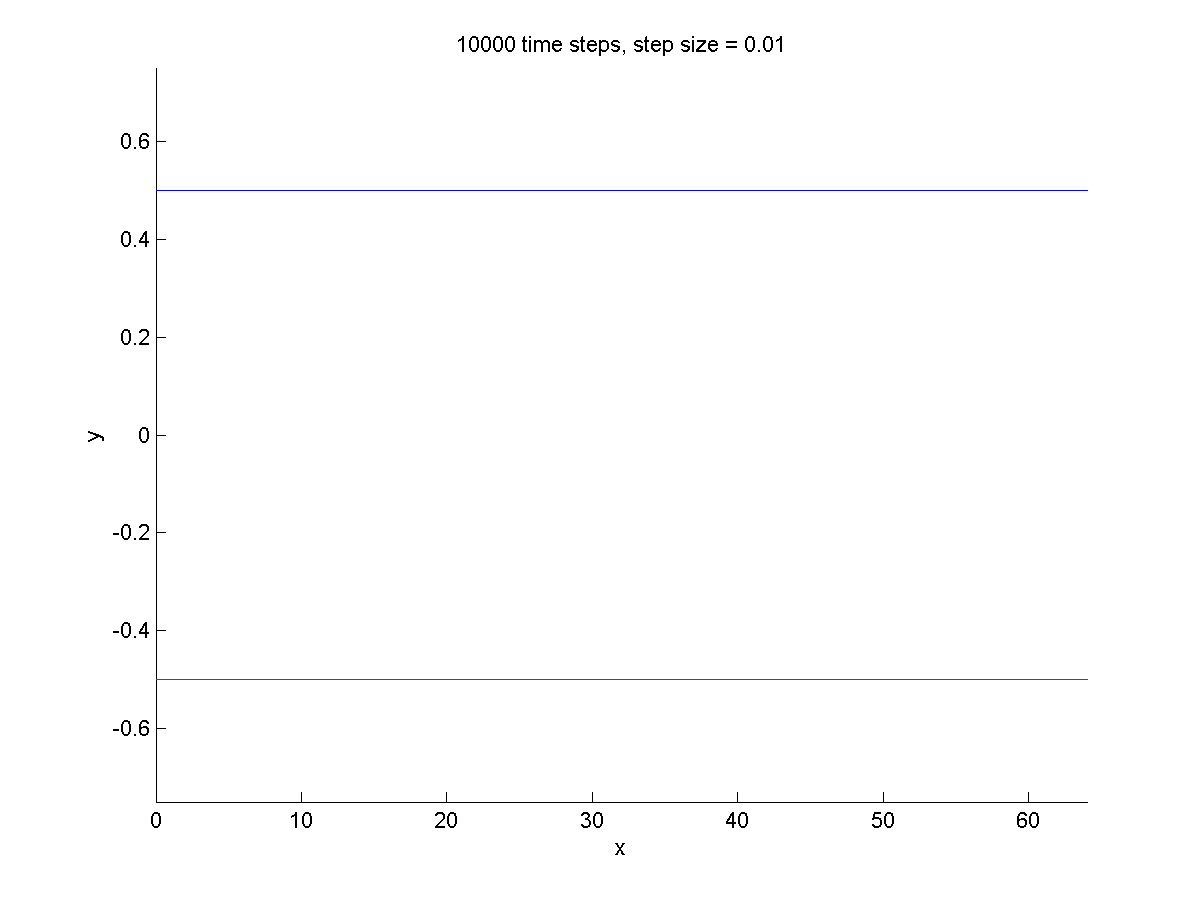
\includegraphics[width=\textwidth]{2vort}
\caption{Interaction of two line vortices of opposite polarity, representing a single vortex ring.}
\label{fig:2vort}
\end{figure}

The mentions of the two-ring interaction made by \citeauthor{helmholtz67} were not a detailed description of the motion of this system, and this was the basis for a paper by \citet{love94}.
\citeauthor{love94} modelled the system also as that of line vortices, with two pairs symmetrically arranged about the $x$ axis, with opposite polarity either side, as in \cref{fig:lovevort}.
\begin{figure}[ht]
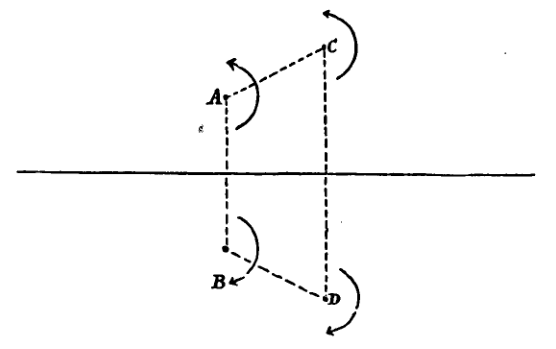
\includegraphics[width=\textwidth]{lovevort}
\caption{Point vortex pairs (A-B and C-D), from \citet[p.186]{love94}}
\label{fig:lovevort}
\end{figure}
If the vortex coordinates are
\begin{align}
\mbox{A:}&\hspace{0.5in}(x_0,y_0)\\
\mbox{B:}&\hspace{0.5in}(x_0,-y_0)\\
\mbox{C:}&\hspace{0.5in}(x_1,y_1)\\
\mbox{D:}&\hspace{0.5in}(x_1,-y_1)
\end{align}
and they have strengths $k$ (A and C) and $-k$ (B and D), then the motion of the fluid can be described by a streamfunction
\begin{equation}
\psi(x,y)=\frac{k}{2\pi}\ln\left(\frac{(x-x_0)^2 + (y+y_0)^2}{(x-x_0)^2 + (y-y_0)^2}\right) + \frac{k}{2\pi}\ln\left(\frac{(x-x_1)^2 + (y+y_1)^2}{(x-x_1)^2 + (y-y_1)^2}\right)
\label{eq:lovesf}
\end{equation}
\citep{love94}.

Now, with the aim of using the definitions of the streamfunction (\cref{eq:sf1,eq:sf2}), we differentiate \cref{eq:lovesf} with respect to $y$
\begin{align}
\partial_y \psi = \frac{k}{\pi}&\left(\frac{y+y_0}{(x-x_0)^2 + (y+y_0)^2}-\frac{y-y_0}{(x-x_0)^2 + (y-y_0)^2}\right.\nonumber\\&\left.+\frac{y+y_1}{(x-x_1)^2 + (y+y_1)^2}-\frac{y-y_1}{(x-x_1)^2 + (y-y_1)^2}\right),
\label{eq:lovesfdy}
\end{align}
and with respect to $x$
\begin{align}
\partial_x \psi = \frac{k}{\pi}&\left(\frac{x-x_0}{(x-x_0)^2 + (y+y_0)^2}-\frac{x-x_0}{(x-x_0)^2 + (y-y_0)^2}\right.\nonumber\\&\left.+\frac{x-x_1}{(x-x_1)^2 + (y+y_1)^2}-\frac{x-x_1}{(x-x_1)^2 + (y-y_1)^2}\right).
\label{eq:lovesfdx}
\end{align}
Now, we wish for the velocity of the vortices, i.e. we are looking at the above equations when $(x,y)\rightarrow(x_0,y_0)$ (or $(x_1,y_1)$).
Again following \citeauthor{love94}, we remove the terms that become infinite in this limit, thus obtaining,
\begin{alignat}{3}
\frac{dx_0}{dt}&=u_x (x_0,y_0)&&= \frac{k}{\pi} \left( \frac{y_1-y_0}{(x_0-x_1)^2 + (y_0-y_1)^2} + \frac{y_0+y_1}{(x_0-x_1)^2 +(y_0+y_1)^2} + \frac{1}{2y_0}\right),\label{eq:vortm1}\\
\frac{dy_0}{dt}&=u_y (x_0,y_0)&&= \frac{k}{\pi} \left( \frac{x_0-x_1}{(x_0-x_1)^2 + (y_0-y_1)^2} + \frac{x_1-x_0}{(x_0-x_1)^2 +(y_0+y_1)^2}\right),\label{eq:vortm2}\\
\frac{dx_1}{dt}&=u_x (x_1,y_1)&&= \frac{k}{\pi} \left( \frac{y_0-y_1}{(x_1-x_0)^2 + (y_1-y_0)^2} + \frac{y_1+y_0}{(x_1-x_0)^2 +(y_1+y_0)^2} + \frac{1}{2y_1}\right),\label{eq:vortm3}\\
\frac{dy_1}{dt}&=u_y (x_1,y_1)&&= \frac{k}{\pi} \left( \frac{x_1-x_0}{(x_1-x_0)^2 + (y_1-y_0)^2} + \frac{x_0-x_1}{(x_1-x_0)^2 +(y_1+y_0)^2} \right).\label{eq:vortm4}
\end{alignat}

\citet{acheson00} generalised these equations for a system of $N$ vortices (with strengths $k_1,k_2,\ldots ,k_N$), obtaining
\begin{align}
\frac{dx_i}{dt}&=\sum^N_{\substack{j=1\\j\neq i}} k_j \frac{y_j - y_i}{(x_i - x_j)^2 + (y_i - y_j)^2},\label{eq:vortposx}\\
\frac{dy_i}{dt}&=\sum^N_{\substack{j=1\\j\neq i}} k_j \frac{x_i - x_j}{(x_i - x_j)^2 + (y_i - y_j)^2},\label{eq:vortposy}
\end{align}
for $i=1,2,\ldots, N$.
The summations in \cref{eq:vortposx,eq:vortposy} are implemented in \hyperref[vortexf]{\texttt{vortexf.m}} and \hyperref[vortexg]{\texttt{vortexg.m}} respectively.

\section{Conserved Quantities}
Returning to \crefrange{eq:vortm1}{eq:vortm4}, and again following \citeauthor{love94}, we can express the right hand side of each equation by the partial derivative of some function $\chi$ (related to the streamfunction $\psi$), with respect to one of the vortex coordinates $x_0,x_1,y_0$ or $y_1$.
\citeauthor{love94} says the differential equations can ``clearly'' be put in the form
\begin{equation}
\frac{dx_0}{\partial_{y_0}\chi}=\frac{dy_0}{-\partial_{x_0}\chi}=\frac{dx_1}{\partial_{y_1}\chi}=\frac{dy_1}{-\partial_{x_1}\chi}=dt.
\label{eq:lovechi}
\end{equation}
To find this function, we must integrate the right hand side as follows:
\begin{itemize}
\item For \cref{eq:vortm1}, we integrate with respect to $y_0$:
\begin{align}
\chi &=\frac{k}{\pi}\int \frac{y_1-y_0}{(x_0-x_1)^2 + (y_0-y_1)^2} + \frac{y_0+y_1}{(x_0-x_1)^2 +(y_0+y_1)^2} + \frac{1}{2y_0}dy_0\nonumber\\
&= \frac{k}{\pi} \left( \int  \frac{y_1-y_0}{(x_0-x_1)^2 + (y_0-y_1)^2} dy_0\right. \nonumber\\ &\left.+ \int \frac{y_0+y_1}{(x_0-x_1)^2 +(y_0+y_1)^2} dy_0 + \int \frac{1}{2y_0}dy_0\right)\nonumber\\
&= \frac{k}{\pi}\left(\inv{2} \ln y_0 -\half \ln((y_0-y_1)^2 +(x_0-x_1)^2)\right. \nonumber\\ &\left. + \half \ln((y_0+y_1)^2 +(x_0-x_1)^2) +C_1 (x_0,x_1,y_1)\right)\nonumber\\
&=\frac{k}{2\pi}\ln y_0 \frac{(y_0+y_1)^2 +(x_0-x_1)^2}{(y_0-y_1)^2 +(x_0-x_1)^2}\cdot C_1 \label{eq:chi1}
\end{align}
\item For \cref{eq:vortm2}, we integrate the negative with respect to $x_0$:
\begin{align}
\chi &=-\frac{k}{\pi}\int \frac{x_0-x_1}{(x_0-x_1)^2 + (y_0-y_1)^2} - \frac{x_0-x_1}{(x_0-x_1)^2 +(y_0+y_1)^2} dx_0\nonumber\\
&= -\frac{k}{\pi} \left( \int  \frac{x_0-x_1}{(x_0-x_1)^2 + (y_0-y_1)^2} dx_0\right. \nonumber\\ &\left.- \int \frac{x_0-x_1}{(x_0-x_1)^2 +(y_0+y_1)^2} dx_0 \right)\nonumber\\
&= \frac{k}{\pi}\left(-\half \ln((y_0-y_1)^2 +(x_0-x_1)^2)\right. \nonumber\\ &\left. + \half \ln((y_0+y_1)^2 +(x_0-x_1)^2) +C_2 (x_1,y_0,y_1)\right)\nonumber\\
&=\frac{k}{2\pi}\ln \frac{(y_0+y_1)^2 +(x_0-x_1)^2}{(y_0-y_1)^2 +(x_0-x_1)^2}\cdot C_2 \label{eq:chi2}
\end{align}
\item For \cref{eq:vortm3}, we integrate with respect to $y_1$:
\begin{align}
\chi &=\frac{k}{\pi}\int \frac{y_0-y_1}{(x_1-x_0)^2 + (y_1-y_0)^2} + \frac{y_0+y_1}{(x_1-x_0)^2 +(y_0+y_1)^2} + \frac{1}{2y_1}dy_1\nonumber\\
&= \frac{k}{\pi} \left( \int  \frac{y_0-y_1}{(x_1-x_0)^2 + (y_1-y_0)^2} dy_1\right. \nonumber\\ &\left.+ \int \frac{y_0+y_1}{(x_1-x_0)^2 +(y_0+y_1)^2} dy_1 + \int \frac{1}{2y_1}dy_0\right)\nonumber\\
&= \frac{k}{\pi}\left(\inv{2} \ln y_1 -\half \ln((y_1-y_0)^2 +(x_1-x_0)^2)\right. \nonumber\\ &\left. + \half \ln((y_0+y_1)^2 +(x_1-x_0)^2) +C_3 (x_0,x_1,y_0)\right)\nonumber\\
&=\frac{k}{2\pi}\ln y_1 \frac{(y_0+y_1)^2 +(x_1-x_0)^2}{(y_1-y_0)^2 +(x_1-x_0)^2} \cdot C_3\label{eq:chi3}
\end{align} 
\item For \cref{eq:vortm4}, we integrate the negative with respect to $x_1$:
\begin{align}
\chi &=-\frac{k}{\pi}\int \frac{x_1-x_0}{(x_1-x_0)^2 + (y_1-y_0)^2} - \frac{x_1-x_0}{(x_1-x_0)^2 +(y_0+y_1)^2} dx_1\nonumber\\
&= -\frac{k}{\pi} \left( \int  \frac{x_1-x_0}{(x_1-x_0)^2 + (y_1-y_0)^2} dx_1\right. \nonumber\\ &\left.- \int \frac{x_1-x_0}{(x_1-x_0)^2 +(y_0+y_1)^2} dx_1 \right)\nonumber\\
&= \frac{k}{\pi}\left(-\half \ln((y_1-y_0)^2 +(x_1-x_0)^2)\right. \nonumber\\ &\left. + \half \ln((y_0+y_1)^2 +(x_1-x_0)^2) +C_4 (x_0,y_0,y_1)\right)\nonumber\\
&=\frac{k}{2\pi}\ln \frac{(y_0+y_1)^2 +(x_1-x_0)^2}{(y_1-y_0)^2 +(x_1-x_0)^2} \cdot C_4\label{eq:chi4}
\end{align}
\end{itemize}
Combining \crefrange{eq:chi1}{eq:chi4}, we can see that, noting that $(a-b)^2 = (b-a)^2$, we must have, for all equations to be equal
\begin{align}
C_1&=y_1,\\
C_3&=y_0,\\
C_2&=C_4=y_1 y_2.
\end{align}
So, we have
\begin{equation}
\chi=\frac{k}{2\pi}\ln y_0 y_1 \frac{(y_0+y_1)^2 +(x_1-x_0)^2}{(y_1-y_0)^2 +(x_1-x_0)^2},
\label{eq:chifinal}
\end{equation}
which agrees with the result in \citet{love94}.

Now we have found $\chi$, we can use it (with \crefrange{eq:vortm1}{eq:vortm4}) to derive the conserved analogues of energy and momentum, as stated in \citet{love94}.
Equating the $dy_0$ and the $dy_1$ parts of \cref{eq:lovechi}, we have
\begin{align}
\frac{dy_0}{-\partial_{x_0}\chi} &= \frac{-dy_1}{\partial_{x_1} \chi},\\
\Rightarrow \frac{\dxb \chi\cdot dy_0 + \dxa \chi \cdot dy_1}{-\partial_{x_0 x_1} \chi}&=0,\\
\Rightarrow \dxb \chi\cdot dy_0 + \dxa \chi \cdot dy_1 &=0,
\end{align}
and, as
\begin{equation}
\dxb \chi = \dxa \chi,
\end{equation}
we have
\begin{align}
dy_0 + dy_1 &=0\\
\Rightarrow y_0 + y_1 &= \mbox{CONSTANT},
\end{align}
as in the paper.

Now equating the $y_0$ and the $x_0$ terms, we have
\begin{align}
\frac{dy_0}{-\dxa \chi} &= \frac{dx_0}{\dya \chi},\\
\Rightarrow \dya \chi dy_0 &= - \dxa \chi dx_0,\\
\Rightarrow \int d\chi &= - \int d\chi,\\
\Rightarrow \chi +c_1 &= -\chi + c_2,\\
\Rightarrow \chi &= \mbox{CONSTANT}.
\end{align}
\begin{figure}
	\centering
	\newlength\figureheight 
	\newlength\figurewidth 
	\setlength\figureheight{10cm} 
	\setlength\figurewidth{\textwidth}
	% This file was created by matlab2tikz.
% Minimal pgfplots version: 1.3
%
%The latest updates can be retrieved from
%  http://www.mathworks.com/matlabcentral/fileexchange/22022-matlab2tikz
%where you can also make suggestions and rate matlab2tikz.
%
\definecolor{mycolor1}{rgb}{0.00000,1.00000,1.00000}%
%
\begin{tikzpicture}

\begin{axis}[%
width=0.95092\figurewidth,
height=\figureheight,
at={(0\figurewidth,0\figureheight)},
scale only axis,
every outer x axis line/.append style={black},
every x tick label/.append style={font=\color{black}},
xmin=0,
xlabel={x},
every outer y axis line/.append style={black},
every y tick label/.append style={font=\color{black}},
ymin=-1.5,
ymax=1.5,
ylabel={y},
title={1000 time steps, step size = 0.001},
axis x line*=bottom,
axis y line*=left
]
\addplot [color=blue,solid,forget plot]
  table[row sep=crcr]{%
0	1\\
-0.000101972060312961	0.999999283100962\\
-0.000203936479754901	0.999996903071822\\
-0.000305886119483717	0.999992859997063\\
-0.000407813841946244	0.999987154015588\\
-0.000509712511555156	0.999979785320695\\
-0.000611574995365235	0.999970754160037\\
-0.000713394163748768	0.999960060835573\\
-0.000815162891069857	0.999947705703506\\
-0.000916874056357391	0.999933689174214\\
-0.00101852054397647	0.999918011712163\\
-0.00112009524429804	0.999900673835812\\
-0.00122159105436651	0.999881676117507\\
-0.00132300087856516	0.999861019183364\\
-0.00142431762927903	0.999838703713137\\
-0.00152553422755518	0.99981473044008\\
-0.00162664360376001	0.999789100150796\\
-0.00172763869823346	0.999761813685071\\
-0.00182851246193989	0.999732871935705\\
-0.00192925785711533	0.999702275848323\\
-0.0020298678579111	0.999670026421184\\
-0.00213033545103324	0.999636124704972\\
-0.00223065363637798	0.999600571802581\\
-0.00233081542766264	0.999563368868888\\
-0.00243081385305203	0.999524517110515\\
-0.00253064195578001	0.999484017785581\\
-0.00263029279476609	0.999441872203447\\
-0.00272975944522681	0.999398081724442\\
-0.0028290349992818	0.999352647759593\\
-0.00292811256655423	0.999305571770332\\
-0.00302698527476555	0.999256855268199\\
-0.0031256462703243	0.99920649981454\\
-0.0032240887189088	0.999154507020183\\
-0.00332230580604366	0.999100878545122\\
-0.00342029073766972	0.999045616098175\\
-0.00351803674070755	0.998988721436645\\
-0.00361553706361405	0.998930196365965\\
-0.00371278497693223	0.998870042739341\\
-0.00380977377383391	0.99880826245738\\
-0.00390649677065521	0.998744857467713\\
-0.00400294730742467	0.998679829764613\\
-0.00409911874838391	0.998613181388596\\
-0.00419500448250065	0.998544914426024\\
-0.00429059792397401	0.998475031008696\\
-0.00438589251273193	0.99840353331343\\
-0.00448088171492053	0.998330423561642\\
-0.00457555902338552	0.998255704018916\\
-0.00466991795814521	0.998179376994563\\
-0.00476395206685533	0.998101444841183\\
-0.00485765492526539	0.998021909954211\\
-0.00495102013766652	0.99794077477146\\
-0.00504404133733071	0.997858041772664\\
-0.00513671218694135	0.997773713479003\\
-0.005229026379015	0.997687792452632\\
-0.00532097763631432	0.997600281296203\\
-0.00541255971225211	0.997511182652378\\
-0.00550376639128627	0.99742049920334\\
-0.00559459148930584	0.997328233670297\\
-0.00568502885400782	0.997234388812988\\
-0.00577507236526494	0.99713896742917\\
-0.00586471593548414	0.997041972354118\\
-0.00595395350995587	0.99694340646011\\
-0.00604277906719407	0.99684327265591\\
-0.00613118661926687	0.996741573886249\\
-0.00621917021211794	0.996638313131303\\
-0.00630672392587844	0.996533493406164\\
-0.00639384187516968	0.996427117760313\\
-0.00648051820939627	0.996319189277087\\
-0.00656674711302994	0.996209711073143\\
-0.00665252280588397	0.996098686297921\\
-0.00673783954337811	0.995986118133104\\
-0.00682269161679425	0.995872009792077\\
-0.00690707335352252	0.995756364519382\\
-0.00699097911729814	0.995639185590173\\
-0.00707440330842886	0.995520476309669\\
-0.00715734036401303	0.995400240012607\\
-0.00723978475814837	0.995278480062689\\
-0.00732173100213149	0.995155199852035\\
-0.00740317364464807	0.995030402800632\\
-0.0074841072719539	0.994904092355779\\
-0.00756452650804666	0.994776271991537\\
-0.00764442601482865	0.99464694520818\\
-0.0077238004922604	0.994516115531634\\
-0.00780264467850517	0.994383786512933\\
-0.00788095335006464	0.994249961727664\\
-0.00795872132190547	0.994114644775415\\
-0.00803594344757718	0.993977839279224\\
-0.00811261461932115	0.993839548885032\\
-0.00818872976817085	0.993699777261129\\
-0.00826428386404354	0.993558528097609\\
-0.00833927191582327	0.993415805105826\\
-0.00841368897143547	0.993271612017841\\
-0.00848753011791298	0.993125952585888\\
-0.00856079048145393	0.992978830581824\\
-0.00863346522747117	0.992830249796594\\
-0.00870554956063365	0.992680214039691\\
-0.00877703872489971	0.99252872713862\\
-0.00884792800354228	0.992375792938364\\
-0.00891821271916635	0.992221415300857\\
-0.00898788823371846	0.992065598104449\\
-0.00905694994848865	0.991908345243385\\
-0.00912539330410469	0.99174966062728\\
-0.00919321378051889	0.991589548180599\\
-0.00926040689698745	0.991428011842141\\
-0.0093269682120426	0.991265055564523\\
-0.00939289332345745	0.991100683313671\\
-0.00945817786820388	0.990934899068314\\
-0.00952281752240336	0.990767706819475\\
-0.00958680800127101	0.990599110569979\\
-0.00965014505905284	0.990429114333947\\
-0.00971282448895637	0.990257722136312\\
-0.00977484212307483	0.990084938012325\\
-0.0098361938323048	0.98991076600707\\
-0.0098968755262577	0.989735210174988\\
-0.00995688315316503	0.989558274579393\\
-0.0100162126997776	0.989379963292006\\
-0.0100748601912589	0.989200280392484\\
-0.0101328216910724	0.989019229967955\\
-0.0101900933008633	0.98883681611256\\
-0.0102466711603351	0.988653042927001\\
-0.01030255144712	0.988467914518084\\
-0.0103577303766442	0.988281434998278\\
-0.0104122042019885	0.988093608485273\\
-0.0104659692137429	0.987904439101544\\
-0.0105190217398571	0.987713930973918\\
-0.0105713581454855	0.987522088233148\\
-0.0106229748328278	0.987328915013493\\
-0.0106738682409649	0.987134415452297\\
-0.0107240348456902	0.986938593689581\\
-0.0107734711593365	0.986741453867634\\
-0.0108221737305991	0.986543000130611\\
-0.0108701391443539	0.986343236624138\\
-0.0109173640214723	0.986142167494916\\
-0.0109638450186317	0.985939796890341\\
-0.0110095788281222	0.985736128958115\\
-0.0110545621776501	0.985531167845876\\
-0.0110987918301371	0.985324917700822\\
-0.0111422645835168	0.985117382669348\\
-0.011184977270527	0.984908566896686\\
-0.0112269267584999	0.984698474526545\\
-0.0112681099491479	0.984487109700764\\
-0.0113085237783474	0.98427447655897\\
-0.0113481652159195	0.984060579238229\\
-0.011387031265407	0.983845421872723\\
-0.0114251189638505	0.98362900859341\\
-0.0114624253815601	0.983411343527708\\
-0.0114989476218855	0.983192430799171\\
-0.0115346828209841	0.982972274527179\\
-0.0115696281475859	0.982750878826627\\
-0.0116037808027569	0.982528247807624\\
-0.0116371380196604	0.982304385575192\\
-0.011669697063316	0.982079296228978\\
-0.0117014552303567	0.981852983862963\\
-0.0117324098487852	0.981625452565178\\
-0.0117625582777268	0.981396706417434\\
-0.0117918979071824	0.981166749495041\\
-0.0118204261577792	0.980935585866548\\
-0.0118481404805198	0.980703219593477\\
-0.0118750383565305	0.980469654730067\\
-0.0119011172968084	0.980234895323026\\
-0.0119263748419665	0.979998945411277\\
-0.011950808561979	0.979761809025722\\
-0.011974416055925	0.979523490189003\\
-0.0119971949517309	0.979283992915272\\
-0.0120191429059128	0.97904332120996\\
-0.0120402576033176	0.978801479069558\\
-0.012060536756864	0.978558470481399\\
-0.0120799781072823	0.978314299423447\\
-0.012098579422854	0.978068969864083\\
-0.0121163384991513	0.97782248576191\\
-0.0121332531587755	0.977574851065549\\
-0.0121493212510961	0.977326069713448\\
-0.0121645406519886	0.97707614563369\\
-0.012178909263573	0.976825082743812\\
-0.0121924250139523	0.976572884950621\\
-0.0122050858569497	0.97631955615002\\
-0.0122168897718477	0.976065100226839\\
-0.0122278347631259	0.975809521054664\\
-0.0122379188601998	0.975552822495676\\
-0.0122471401171592	0.975295008400494\\
-0.0122554966125071	0.975036082608018\\
-0.0122629864488998	0.974776048945285\\
-0.0122696077528856	0.974514911227315\\
-0.0122753586746459	0.974252673256976\\
-0.0122802373877354	0.973989338824844\\
-0.0122842420888235	0.973724911709069\\
-0.0122873709974362	0.973459395675249\\
-0.0122896223556987	0.973192794476298\\
-0.0122909944280784	0.97292511185233\\
-0.0122914855011292	0.972656351530538\\
-0.012291093883236	0.972386517225081\\
-0.0122898179043602	0.972115612636974\\
-0.0122876559157867	0.971843641453979\\
-0.0122846062898706	0.971570607350506\\
-0.0122806674197859	0.971296513987508\\
-0.012275837719275	0.97102136501239\\
-0.0122701156223984	0.970745164058913\\
-0.0122634995832868	0.970467914747107\\
-0.0122559880758931	0.970189620683183\\
-0.0122475795937462	0.969910285459453\\
-0.0122382726497057	0.969629912654252\\
-0.0122280657757179	0.969348505831855\\
-0.0122169575225729	0.969066068542414\\
-0.0122049464596632	0.96878260432188\\
-0.012192031174743	0.968498116691944\\
-0.0121782102736894	0.968212609159966\\
-0.0121634823802648	0.967926085218919\\
-0.0121478461358801	0.967638548347333\\
-0.0121313001993602	0.967350002009236\\
-0.01211384324671	0.967060449654105\\
-0.0120954739708823	0.966769894716815\\
-0.0120761910815469	0.966478340617595\\
-0.0120559933048616	0.966185790761984\\
-0.0120348793832437	0.965892248540788\\
-0.0120128480751443	0.965597717330044\\
-0.0119898981548227	0.965302200490985\\
-0.0119660284121235	0.965005701370002\\
-0.0119412376522542	0.96470822329862\\
-0.0119155246955655	0.964409769593464\\
-0.0118888883773319	0.964110343556236\\
-0.0118613275475347	0.963809948473691\\
-0.0118328410706463	0.963508587617616\\
-0.0118034278254162	0.963206264244808\\
-0.0117730867046582	0.962902981597064\\
-0.0117418166150397	0.962598742901156\\
-0.0117096164768726	0.96229355136883\\
-0.0116764852239049	0.961987410196786\\
-0.0116424218031155	0.961680322566676\\
-0.011607425174509	0.961372291645092\\
-0.0115714943109135	0.961063320583567\\
-0.0115346281977787	0.96075341251857\\
-0.0114968258329771	0.960442570571502\\
-0.0114580862266055	0.960130797848705\\
-0.011418408400789	0.959818097441456\\
-0.0113777913894862	0.959504472425978\\
-0.0113362342382965	0.959189925863444\\
-0.0112937360042684	0.958874460799986\\
-0.0112502957557101	0.958558080266703\\
-0.0112059125720011	0.958240787279673\\
-0.0111605855434063	0.957922584839969\\
-0.0111143137708907	0.957603475933667\\
-0.0110670963659368	0.957283463531868\\
-0.0110189324503626	0.956962550590714\\
-0.0109698211561422	0.956640740051403\\
-0.0109197616252272	0.956318034840215\\
-0.0108687530093705	0.955994437868529\\
-0.0108167944699512	0.955669952032849\\
-0.010763885177801	0.955344580214824\\
-0.010710024313033	0.95501832528128\\
-0.0106552110648712	0.95469119008424\\
-0.0105994446314821	0.954363177460957\\
-0.010542724219808	0.954034290233941\\
-0.0104850490454015	0.953704531210987\\
-0.0104264183322618	0.953373903185211\\
-0.0103668313126727	0.953042408935078\\
-0.0103062872270418	0.95271005122444\\
-0.0102447853237421	0.952376832802564\\
-0.0101823248589537	0.952042756404176\\
-0.0101189050965087	0.95170782474949\\
-0.0100545253077366	0.951372040544248\\
-0.00998918477131149	0.951035406479759\\
-0.00992288277310073	0.95069792523294\\
-0.00985561860601536	0.950359599466351\\
-0.0097873915698618	0.950020431828239\\
-0.00971820097119514	0.949680424952581\\
-0.00964804612317389	0.949339581459124\\
-0.00957692634541625	0.948997903953429\\
-0.0095048409638578	0.948655395026915\\
-0.0094317893106107	0.948312057256906\\
-0.00935777072382435	0.947967893206671\\
-0.00928278454754741	0.947622905425476\\
-0.00920683013159138	0.947277096448627\\
-0.00912990683139547	0.94693046879752\\
-0.00905201400789299	0.946583024979686\\
-0.00897315102737906	0.946234767488842\\
-0.00889331726137978	0.945885698804939\\
-0.0088125120865227	0.945535821394213\\
-0.00873073488440877	0.945185137709232\\
-0.00864798504148548	0.94483365018895\\
-0.00856426194892155	0.94448136125876\\
-0.00847956500248276	0.944128273330538\\
-0.00839389360240925	0.943774388802704\\
-0.00830724715329407	0.943419710060269\\
-0.00821962506396299	0.943064239474889\\
-0.00813102674735572	0.942707979404921\\
-0.00804145162040825	0.942350932195473\\
-0.0079508991039366	0.941993100178462\\
-0.00785936862252175	0.941634485672664\\
-0.00776685960439579	0.941275090983774\\
-0.00767337148132939	0.940914918404459\\
-0.00757890368852043	0.94055397021441\\
-0.00748345566448379	0.940192248680404\\
-0.00738702685094247	0.939829756056357\\
-0.00728961669271977	0.939466494583378\\
-0.00719122463763271	0.939102466489831\\
-0.00709185013638658	0.938737673991387\\
-0.00699149264247066	0.938372119291085\\
-0.00689015161205508	0.938005804579384\\
-0.00678782650388876	0.937638732034229\\
-0.00668451677919857	0.937270903821098\\
-0.00658022190158946	0.936902322093069\\
-0.00647494133694579	0.936532988990875\\
-0.00636867455333367	0.936162906642958\\
-0.00626142102090444	0.935792077165535\\
-0.0061531802117991	0.93542050266265\\
-0.00604395160005391	0.935048185226237\\
-0.00593373466150696	0.934675126936175\\
-0.00582252887370573	0.934301329860352\\
-0.00571033371581575	0.933926796054717\\
-0.00559714866853015	0.933551527563345\\
-0.00548297321398036	0.933175526418493\\
-0.00536780683564757	0.932798794640662\\
-0.0052516490182754	0.93242133423865\\
-0.0051344992477833	0.932043147209622\\
-0.00501635701118106	0.931664235539156\\
-0.00489722179648419	0.931284601201315\\
-0.0047770930926302	0.930904246158698\\
-0.00465597038939587	0.930523172362503\\
-0.0045338531773153	0.930141381752586\\
-0.00441074094759901	0.929758876257519\\
-0.00428663319205377	0.929375657794651\\
-0.00416152940300339	0.928991728270169\\
-0.00403542907321036	0.928607089579153\\
-0.00390833169579832	0.928221743605639\\
-0.00378023676417535	0.927835692222679\\
-0.00365114377195816	0.927448937292395\\
-0.00352105221289701	0.927061480666047\\
-0.00338996158080152	0.926673324184084\\
-0.00325787136946722	0.926284469676207\\
-0.00312478107260292	0.92589491896143\\
-0.00299069018375886	0.925504673848136\\
-0.0028555981962556	0.925113736134138\\
-0.00271950460311371	0.924722107606735\\
-0.00258240889698419	0.924329790042776\\
-0.00244431057007964	0.923936785208715\\
-0.00230520911410611	0.923543094860672\\
-0.0021651040201958	0.92314872074449\\
-0.00202399477884029	0.922753664595795\\
-0.00188188087982468	0.922357928140054\\
-0.00173876181216223	0.921961513092633\\
-0.00159463706402984	0.921564421158857\\
-0.00144950612270408	0.921166654034066\\
-0.00130336847449803	0.920768213403677\\
-0.00115622360469864	0.920369100943237\\
-0.00100807099750482	0.919969318318485\\
-0.000858910135966165	0.919568867185408\\
-0.000708740501922288	0.9191677491903\\
-0.000557561575942813	0.918765965969819\\
-0.000405372837267957	0.918363519151043\\
-0.000252173763749736	0.917960410351531\\
-9.79638317937697e-005	0.917556641179378\\
5.72574836983243e-005	0.91715221323327\\
0.000213490709385943	0.916747128102548\\
0.000370736373545937	0.916341387367256\\
0.000528995006128485	0.915934992598205\\
0.000688267138812393	0.915527945357028\\
0.000848553305059848	0.915120247196232\\
0.00100985404017062	0.914711899659261\\
0.00117216988133575	0.914302904280549\\
0.00133550136769062	0.913893262585576\\
0.00149984904036763	0.913482976090924\\
0.00166521344254823	0.913072046304334\\
0.00183159511951454	0.912660474724761\\
0.00199899461870039	0.912248262842432\\
0.00216741248974188	0.911835412138896\\
0.0023368492845275	0.911421924087084\\
0.00250730555724771	0.911007800151364\\
0.00267878186444404	0.910593041787594\\
0.00285127876505778	0.910177650443177\\
0.0030247968204781	0.90976162755712\\
0.00319933659458985	0.909344974560082\\
0.00337489865382078	0.908927692874433\\
0.00355148356718836	0.908509783914307\\
0.00372909190634619	0.908091249085658\\
0.00390772424562997	0.907672089786312\\
0.00408738116210297	0.90725230740602\\
0.00426806323560115	0.906831903326516\\
0.00444977104877786	0.906410878921565\\
0.00463250518714811	0.905989235557023\\
0.00481626623913242	0.905566974590885\\
0.00500105479610028	0.905144097373341\\
0.00518687145241325	0.904720605246827\\
0.00537371680546763	0.904296499546082\\
0.00556159145573674	0.903871781598196\\
0.00575049600681287	0.903446452722666\\
0.0059404310654488	0.903020514231447\\
0.00613139724159899	0.902593967429007\\
0.0063233951484604	0.902166813612374\\
0.00651642540251291	0.901739054071194\\
0.00671048862355947	0.90131069008778\\
0.00690558543476581	0.900881722937165\\
0.00710171646269985	0.900452153887151\\
0.0072988823373708	0.900021984198364\\
0.00749708369226784	0.899591215124307\\
0.00769632116439854	0.899159847911405\\
0.00789659539432695	0.898727883799063\\
0.00809790702621132	0.898295324019711\\
0.00830025670784153	0.897862169798862\\
0.00850364509067623	0.897428422355156\\
0.00870807282987961	0.896994082900416\\
0.00891354058435794	0.896559152639696\\
0.00912004901679572	0.896123632771332\\
0.00932759879369161	0.895687524486991\\
0.00953619058539402	0.895250828971726\\
0.00974582506613642	0.89481354740402\\
0.00995650291407235	0.894375680955841\\
0.0101682248113102	0.893937230792689\\
0.0103809914439476	0.893498198073647\\
0.0105948035021058	0.893058583951432\\
0.0108096616799631	0.892618389572441\\
0.0110255666757891	0.892177616076804\\
0.0112425191919777	0.891736264598432\\
0.0114605199350802	0.891294336265066\\
0.0116795696158383	0.890851832198329\\
0.0118996689492167	0.890408753513769\\
0.0121208186544352	0.889965101320914\\
0.0123430194550009	0.88952087672332\\
0.0125662720787403	0.889076080818616\\
0.0127905772578304	0.888630714698556\\
0.0130159357288304	0.888184779449067\\
0.0132423482327126	0.887738276150299\\
0.0134698155148935	0.88729120587667\\
0.0136983383252641	0.886843569696917\\
0.0139279174182206	0.886395368674143\\
0.0141585535526943	0.885946603865867\\
0.0143902474921818	0.885497276324069\\
0.0146230000047744	0.885047387095241\\
0.0148568118631879	0.884596937220434\\
0.0150916838447916	0.884145927735306\\
0.0153276167316375	0.883694359670169\\
0.015564611310489	0.883242234050036\\
0.0158026683728496	0.882789551894672\\
0.0160417887149914	0.88233631421864\\
0.0162819731379829	0.881882522031345\\
0.0165232224477174	0.881428176337088\\
0.0167655374549406	0.880973278135107\\
0.017008918975278	0.88051782841963\\
0.0172533678292625	0.880061828179916\\
0.0174988848423614	0.87960527840031\\
0.0177454708450032	0.879148180060283\\
0.0179931266726049	0.878690534134483\\
0.0182418531655979	0.87823234159278\\
0.0184916511694547	0.877773603400316\\
0.0187425215347149	0.87731432051755\\
0.0189944651170113	0.876854493900302\\
0.0192474827770958	0.876394124499807\\
0.0195015753808643	0.875933213262754\\
0.0197567437993829	0.875471761131339\\
0.0200129889089127	0.875009769043309\\
0.0202703115909349	0.874547237932007\\
0.0205287127321753	0.874084168726422\\
0.0207881932246294	0.873620562351235\\
0.0210487539655865	0.873156419726864\\
0.0213103958576543	0.872691741769511\\
0.0215731198087826	0.872226529391209\\
0.0218369267322872	0.87176078349987\\
0.0221018175468739	0.871294504999329\\
0.0223677931766618	0.870827694789391\\
0.0226348545512068	0.87036035376588\\
0.0229030026055246	0.869892482820681\\
0.0231722382801135	0.86942408284179\\
0.0234425625209777	0.86895515471336\\
0.0237139762796495	0.868485699315745\\
0.0239864805132119	0.868015717525551\\
0.0242600761843208	0.867545210215677\\
0.024534764261227	0.867074178255365\\
0.0248105457177982	0.866602622510245\\
0.025087421533541	0.866130543842381\\
0.0253653926936216	0.86565794311032\\
0.025644460188888	0.865184821169135\\
0.0259246250158909	0.864711178870473\\
0.0262058881769046	0.864237017062602\\
0.0264882506799477	0.863762336590455\\
0.0267717135388041	0.86328713829568\\
0.0270562777730432	0.862811423016683\\
0.0273419444080403	0.862335191588677\\
0.0276287144749967	0.861858444843727\\
0.0279165890109593	0.861381183610796\\
0.0282055690588409	0.860903408715794\\
0.0284956556674394	0.86042512098162\\
0.028786849891457	0.859946321228215\\
0.02907915279152	0.859467010272601\\
0.0293725654341971	0.858987188928935\\
0.0296670888920187	0.858506858008549\\
0.0299627242434954	0.858026018320001\\
0.0302594725731363	0.857544670669121\\
0.0305573349714678	0.857062815859057\\
0.0308563125350508	0.856580454690318\\
0.0311564063664995	0.85609758796083\\
0.0314576175744985	0.855614216465974\\
0.0317599472738206	0.855130340998636\\
0.0320633965853441	0.854645962349255\\
0.0323679666360697	0.854161081305868\\
0.0326736585591378	0.853675698654159\\
0.0329804734938452	0.853189815177503\\
0.0332884125856613	0.852703431657016\\
0.0335974769862448	0.852216548871601\\
0.0339076678534598	0.851729167597995\\
0.0342189863513918	0.851241288610816\\
0.0345314336503633	0.85075291268261\\
0.0348450109269497	0.8502640405839\\
0.0351597193639941	0.849774673083232\\
0.035475560150623	0.84928481094722\\
0.0357925344822613	0.8487944549406\\
0.0361106435606463	0.84830360582627\\
0.0364298885938433	0.847812264365345\\
0.036750270796259	0.847320431317196\\
0.0370717913886563	0.846828107439506\\
0.0373944515981677	0.846335293488313\\
0.0377182526583093	0.84584199021806\\
0.0380431958089942	0.84534819838164\\
0.038369282296546	0.844853918730449\\
0.0386965133737111	0.844359152014429\\
0.0390248902996726	0.843863898982117\\
0.0393544143400617	0.843368160380697\\
0.0396850867669713	0.842871936956044\\
0.040016908858967	0.842375229452775\\
0.0403498819010998	0.841878038614295\\
0.0406840071849175	0.841380365182847\\
0.0410192860084761	0.840882209899562\\
0.041355719676351	0.840383573504505\\
0.0416933094996482	0.839884456736723\\
0.0420320567960148	0.839384860334298\\
0.0423719628896493	0.838884785034394\\
0.0427130291113125	0.838384231573301\\
0.0430552567983367	0.837883200686494\\
0.0433986472946361	0.837381693108673\\
0.0437432019507157	0.836879709573816\\
0.0440889221236812	0.83637725081523\\
0.0444358091772474	0.835874317565596\\
0.0447838644817471	0.835370910557022\\
0.0451330894141397	0.834867030521093\\
0.0454834853580192	0.834362678188916\\
0.0458350537036222	0.833857854291175\\
0.0461877958478357	0.833352559558179\\
0.046541713194204	0.832846794719909\\
0.0468968071529364	0.832340560506073\\
0.0472530791409136	0.831833857646153\\
0.0476105305816944	0.831326686869456\\
0.0479691629055221	0.830819048905162\\
0.04832897754933	0.83031094448238\\
0.0486899759567476	0.829802374330192\\
0.0490521595781056	0.829293339177708\\
0.0494155298704414	0.828783839754113\\
0.0497800882975033	0.828273876788723\\
0.0501458363297555	0.82776345101103\\
0.050512775444382	0.827252563150756\\
0.0508809071252908	0.826741213937904\\
0.0512502328631169	0.826229404102809\\
0.051620754155226	0.825717134376187\\
0.0519924725057173	0.82520440548919\\
0.052365389425426	0.824691218173454\\
0.0527395064319257	0.824177573161152\\
0.0531148250495303	0.823663471185047\\
0.0534913468092956	0.82314891297854\\
0.0538690732490207	0.822633899275724\\
0.0542480059132487	0.822118430811438\\
0.0546281463532675	0.821602508321312\\
0.05500949612711	0.821086132541828\\
0.0553920567995539	0.820569304210365\\
0.0557758299421215	0.820052024065254\\
0.0561608171330786	0.819534292845831\\
0.0565470199574337	0.819016111292488\\
0.056934440006936	0.818497480146724\\
0.0573230788800739	0.817978400151202\\
0.0577129381820726	0.817458872049798\\
0.0581040195248914	0.816938896587652\\
0.0584963245272209	0.816418474511227\\
0.0588898548144792	0.815897606568357\\
0.0592846120188085	0.8153762935083\\
0.059680597779071	0.814854536081793\\
0.0600778137408437	0.814332335041105\\
0.0604762615564143	0.813809691140086\\
0.0608759428847751	0.813286605134228\\
0.0612768593916178	0.812763077780711\\
0.0616790127493267	0.812239109838461\\
0.062082404636973	0.811714702068199\\
0.0624870367403068	0.8111898552325\\
0.0628929107517506	0.810664570095843\\
0.0633000283703906	0.810138847424664\\
0.0637083913019693	0.809612687987414\\
0.0641180012588759	0.809086092554608\\
0.0645288599601379	0.80855906189888\\
0.0649409691314113	0.808031596795039\\
0.0653543305049703	0.807503698020122\\
0.0657689458196971	0.806975366353447\\
0.0661848168210711	0.806446602576668\\
0.0666019452611572	0.805917407473827\\
0.0670203328985941	0.805387781831413\\
0.0674399814985822	0.804857726438411\\
0.0678608928328706	0.804327242086358\\
0.0682830686797439	0.803796329569401\\
0.0687065108240086	0.803264989684343\\
0.0691312210569788	0.802733223230706\\
0.0695572011764617	0.802201031010781\\
0.069984452986742	0.801668413829682\\
0.070412978298567	0.801135372495402\\
0.0708427789291298	0.800601907818869\\
0.0712738567020529	0.800068020613995\\
0.0717062134473711	0.799533711697738\\
0.0721398510015139	0.798998981890148\\
0.072574771207287	0.79846383201443\\
0.0730109759138542	0.797928262896993\\
0.0734484669767176	0.797392275367505\\
0.0738872462576982	0.796855870258951\\
0.0743273156249158	0.796319048407684\\
0.074768676952768	0.79578181065348\\
0.0752113321219087	0.795244157839595\\
0.0756552830192267	0.794706090812816\\
0.0761005315378233	0.794167610423518\\
0.0765470795769888	0.793628717525718\\
0.0769949290421797	0.793089412977128\\
0.0774440818449942	0.792549697639212\\
0.0778945399031479	0.792009572377239\\
0.0783463051404484	0.791469038060335\\
0.0787993794867699	0.790928095561541\\
0.0792537648780267	0.790386745757867\\
0.0797094632561462	0.789844989530344\\
0.0801664765690418	0.789302827764077\\
0.0806248067705849	0.788760261348304\\
0.0810844558205758	0.788217291176446\\
0.0815454256847153	0.787673918146162\\
0.0820077183345742	0.787130143159404\\
0.0824713357475634	0.786585967122469\\
0.0829362799069029	0.786041390946053\\
0.0834025528015901	0.785496415545305\\
0.0838701564263677	0.784951041839881\\
0.0843390927816909	0.784405270753998\\
0.0848093638736944	0.783859103216484\\
0.0852809717141577	0.783312540160836\\
0.0857539183204712	0.782765582525268\\
0.0862282057156008	0.782218231252767\\
0.0867038359280518	0.781670487291147\\
0.0871808109918326	0.781122351593097\\
0.0876591329464179	0.78057382511624\\
0.0881388038367107	0.780024908823178\\
0.0886198257130037	0.77947560368155\\
0.0891022006309411	0.778925910664084\\
0.0895859306514782	0.778375830748642\\
0.0900710178408416	0.777825364918282\\
0.0905574642704882	0.777274514161301\\
0.0910452720170636	0.776723279471291\\
0.0915344431623601	0.776171661847187\\
0.0920249797932735	0.775619662293323\\
0.09251688400176	0.775067281819476\\
0.0930101578847919	0.774514521440923\\
0.093504803544313	0.773961382178488\\
0.0940008230871925	0.773407865058589\\
0.09449821862518	0.772853971113297\\
0.0949969922748576	0.772299701380375\\
0.0954971461575934	0.771745056903336\\
0.0959986823994926	0.771190038731486\\
0.0965016031313494	0.770634647919977\\
0.0970059104885974	0.770078885529854\\
0.0975116066112592	0.769522752628102\\
0.0980186936438961	0.768966250287696\\
0.0985271737355564	0.768409379587649\\
0.0990370490397234	0.767852141613057\\
0.0995483217142624	0.767294537455148\\
0.100060993921368	0.76673656821133\\
0.100575067827509	0.766178234985233\\
0.101090545603374	0.76561953888676\\
0.101607429423816	0.765060481032132\\
0.102125721467798	0.764501062543929\\
0.102645423918332	0.763941284551141\\
0.103166538962425	0.76338114818921\\
0.103689068791021	0.762820654600073\\
0.10421301559894	0.762259804932209\\
0.10473838158482	0.76169860034068\\
0.105265168951055	0.761137041987177\\
0.105793379903739	0.760575131040058\\
0.106323016652598	0.760012868674398\\
0.106854081410932	0.759450256072021\\
0.107386576395552	0.758887294421552\\
0.107920503826715	0.758323984918449\\
0.108455865928059	0.75776032876505\\
0.108992664926543	0.757196327170608\\
0.109530903052374	0.756631981351338\\
0.110070582538949	0.756067292530447\\
0.110611705622782	0.755502261938179\\
0.111154274543439	0.754936890811852\\
0.11169829154347	0.754371180395896\\
0.112243758868339	0.753805131941886\\
0.112790678766358	0.753238746708587\\
0.11333905348861	0.752672025961981\\
0.113888885288888	0.752104970975309\\
0.114440176423613	0.751537583029104\\
0.114992929151772	0.750969863411224\\
0.115547145734838	0.750401813416889\\
0.1161028284367	0.749833434348712\\
0.116659979523589	0.749264727516732\\
0.117218601264003	0.748695694238447\\
0.117778695928632	0.748126335838845\\
0.118340265790282	0.747556653650436\\
0.1189033131238	0.74698664901328\\
0.119467840205996	0.746416323275019\\
0.120033849315564	0.745845677790904\\
0.120601342733007	0.745274713923826\\
0.121170322740555	0.744703433044342\\
0.12174079162209	0.7441318365307\\
0.122312751663061	0.74355992576887\\
0.122886205150408	0.742987702152567\\
0.123461154372476	0.742415167083275\\
0.124037601618941	0.741842321970275\\
0.124615549180721	0.741269168230662\\
0.125194999349893	0.740695707289376\\
0.125775954419617	0.740121940579218\\
0.126358416684046	0.739547869540874\\
0.126942388438242	0.738973495622933\\
0.127527871978094	0.738398820281912\\
0.128114869600232	0.737823844982269\\
0.128703383601938	0.737248571196425\\
0.129293416281064	0.736673000404781\\
0.129884969935944	0.736097134095734\\
0.130478046865304	0.735520973765693\\
0.131072649368178	0.734944520919093\\
0.131668779743817	0.734367777068413\\
0.132266440291602	0.733790743734184\\
0.132865633310954	0.733213422445007\\
0.133466361101245	0.732635814737559\\
0.134068625961708	0.73205792215661\\
0.134672430191345	0.731479746255027\\
0.135277776088839	0.730901288593789\\
0.135884665952461	0.73032255074199\\
0.136493102079978	0.72974353427685\\
0.137103086768561	0.729164240783719\\
0.137714622314697	0.728584671856083\\
0.138327711014088	0.728004829095572\\
0.138942355161565	0.727424714111957\\
0.139558557050993	0.726844328523159\\
0.140176318975175	0.726263673955249\\
0.140795643225761	0.725682752042446\\
0.141416532093149	0.725101564427123\\
0.142038987866397	0.724520112759797\\
0.142663012833124	0.723938398699137\\
0.143288609279414	0.723356423911955\\
0.143915779489724	0.722774190073202\\
0.144544525746786	0.722191698865966\\
0.145174850331509	0.721608951981463\\
0.145806755522891	0.721025951119035\\
0.146440243597911	0.720442697986134\\
0.147075316831444	0.719859194298322\\
0.147711977496156	0.719275441779256\\
0.148350227862412	0.718691442160675\\
0.148990070198176	0.718107197182396\\
0.149631506768917	0.717522708592292\\
0.150274539837509	0.716937978146283\\
0.150919171664134	0.716353007608322\\
0.151565404506187	0.715767798750374\\
0.152213240618177	0.715182353352404\\
0.152862682251628	0.714596673202354\\
0.153513731654983	0.714010760096128\\
0.154166391073508	0.713424615837569\\
0.154820662749191	0.71283824223844\\
0.155476548920646	0.712251641118397\\
0.156134051823015	0.711664814304972\\
0.156793173687873	0.711077763633542\\
0.157453916743125	0.710490490947308\\
0.158116283212915	0.709902998097265\\
0.158780275317522	0.709315286942177\\
0.159445895273269	0.708727359348546\\
0.160113145292421	0.708139217190582\\
0.160782027583091	0.707550862350173\\
0.161452544349142	0.706962296716854\\
0.162124697790087	0.706373522187769\\
0.162798490101	0.705784540667643\\
0.163473923472412	0.705195354068741\\
0.16415100009022	0.704605964310835\\
0.164829722135587	0.704016373321164\\
0.16551009178485	0.703426583034397\\
0.166192111209421	0.702836595392594\\
0.166875782575695	0.702246412345162\\
0.167561108044953	0.701656035848815\\
0.168248089773268	0.70106546786753\\
0.168936729911412	0.700474710372506\\
0.16962703060476	0.699883765342114\\
0.170318993993197	0.699292634761853\\
0.171012622211026	0.698701320624303\\
0.171707917386874	0.698109824929076\\
0.172404881643601	0.697518149682767\\
0.173103517098206	0.696926296898902\\
0.173803825861737	0.696334268597886\\
0.1745058100392	0.695742066806953\\
0.175209471729469	0.69514969356011\\
0.175914813025193	0.694557150898083\\
0.176621836012711	0.693964440868258\\
0.177330542771958	0.693371565524631\\
0.178040935376382	0.692778526927741\\
0.178753015892853	0.692185327144618\\
0.179466786381574	0.69159196824872\\
0.180182248895999	0.690998452319872\\
0.180899405482743	0.690404781444202\\
0.181618258181499	0.689810957714084\\
0.182338809024952	0.689216983228065\\
0.183061060038695	0.688622860090807\\
0.183785013241147	0.688028590413018\\
0.184510670643469	0.687434176311383\\
0.185238034249482	0.6868396199085\\
0.185967106055587	0.686244923332808\\
0.186697888050683	0.685650088718516\\
0.187430382216089	0.685055118205535\\
0.188164590525464	0.684460013939403\\
0.18890051494473	0.683864778071216\\
0.189638157431993	0.683269412757549\\
0.190377519937468	0.682673920160384\\
0.191118604403405	0.682078302447034\\
0.191861412764011	0.681482561790069\\
0.192605946945378	0.680886700367231\\
0.19335220886541	0.680290720361364\\
0.194100200433752	0.67969462396033\\
0.194849923551719	0.679098413356931\\
0.195601380112222	0.678502090748825\\
0.196354571999706	0.677905658338449\\
0.197109501090076	0.677309118332931\\
0.197866169250631	0.676712472944012\\
0.198624578340002	0.676115724387956\\
0.199384730208082	0.675518874885471\\
0.200146626695964	0.674921926661617\\
0.200910269635878	0.674324881945725\\
0.20167566085113	0.673727742971307\\
0.20244280215604	0.673130511975968\\
0.203211695355883	0.672533191201317\\
0.203982342246829	0.671935782892879\\
0.204754744615889	0.671338289300003\\
0.205528904240855	0.670740712675775\\
0.206304822890246	0.670143055276919\\
0.207082502323254	0.669545319363713\\
0.207861944289694	0.668947507199892\\
0.208643150529947	0.668349621052556\\
0.209426122774914	0.667751663192074\\
0.210210862745964	0.667153635891992\\
0.210997372154888	0.666555541428937\\
0.211785652703852	0.665957382082521\\
0.212575706085349	0.665359160135244\\
0.213367533982158	0.6647608778724\\
0.2141611380673	0.664162537581975\\
0.214956520003993	0.663564141554556\\
0.215753681445617	0.662965692083227\\
0.21655262403567	0.662367191463472\\
0.217353349407736	0.661768641993077\\
0.218155859185439	0.661170045972031\\
0.218960154982418	0.660571405702424\\
0.219766238402285	0.659972723488346\\
0.220574111038599	0.659374001635791\\
0.221383774474828	0.658775242452553\\
0.222195230284325	0.658176448248121\\
0.223008480030296	0.657577621333587\\
0.223823525265773	0.656978764021532\\
0.22464036753359	0.656379878625936\\
0.225459008366357	0.655780967462066\\
0.226279449286436	0.655182032846377\\
0.227101691805921	0.654583077096411\\
0.227925737426618	0.65398410253069\\
0.228751587640024	0.653385111468617\\
0.22957924392731	0.652786106230367\\
0.230408707759307	0.652187089136791\\
0.231239980596488	0.651588062509304\\
0.232073063888955	0.650989028669787\\
0.232907959076431	0.650389989940482\\
0.233744667588243	0.649790948643885\\
0.23458319084332	0.649191907102646\\
0.235423530250179	0.648592867639464\\
0.236265687206921	0.647993832576981\\
0.237109663101228	0.647394804237679\\
0.237955459310356	0.646795784943777\\
0.238803077201135	0.646196777017125\\
0.239652518129968	0.645597782779103\\
0.240503783442832	0.644998804550514\\
0.241356874475279	0.644399844651482\\
0.242211792552441	0.64380090540135\\
0.243068538989034	0.643201989118573\\
0.243927115089362	0.642603098120617\\
0.244787522147332	0.642004234723854\\
0.245649761446454	0.641405401243462\\
0.246513834259858	0.640806599993322\\
0.247379741850304	0.640207833285911\\
0.248247485470194	0.639609103432207\\
0.24911706636159	0.639010412741578\\
0.249988485756227	0.638411763521692\\
0.25086174487553	0.637813158078404\\
0.251736844930637	0.637214598715662\\
0.252613787122415	0.636616087735406\\
0.253492572641485	0.636017627437465\\
0.25437320266824	0.635419220119458\\
0.255255678372877	0.634820868076694\\
0.256140000915415	0.634222573602078\\
0.257026171445725	0.633624338986003\\
0.257914191103562	0.633026166516261\\
0.258804061018587	0.632428058477938\\
0.259695782310404	0.631830017153322\\
0.260589356088592	0.631232044821804\\
0.261484783452735	0.63063414375978\\
0.262382065492459	0.630036316240561\\
0.263281203287469	0.62943856453427\\
0.264182197907585	0.628840890907754\\
0.265085050412782	0.628243297624487\\
0.265989761853227	0.627645786944477\\
0.266896333269325	0.627048361124175\\
0.267804765691756	0.626451022416377\\
0.268715060141524	0.625853773070141\\
0.269627217629998	0.625256615330691\\
0.27054123915896	0.624659551439325\\
0.27145712572065	0.624062583633332\\
0.272374878297818	0.623465714145896\\
0.27329449786377	0.622868945206015\\
0.274215985382421	0.622272279038406\\
0.275139341808346	0.621675717863427\\
0.276064568086834	0.621079263896982\\
0.276991665153941	0.620482919350445\\
0.277920633936544	0.619886686430567\\
0.278851475352403	0.619290567339401\\
0.27978419031021	0.618694564274213\\
0.280718779709653	0.618098679427402\\
0.281655244441477	0.617502914986422\\
0.282593585387539	0.616907273133696\\
0.283533803420873	0.616311756046542\\
0.284475899405753	0.615716365897092\\
0.285419874197754	0.615121104852216\\
0.286365728643821	0.614525975073442\\
0.287313463582328	0.613930978716886\\
0.288263079843152	0.61333611793317\\
0.289214578247734	0.612741394867355\\
0.290167959609151	0.612146811658863\\
0.291123224732182	0.611552370441407\\
0.292080374413384	0.610958073342922\\
0.293039409441155	0.610363922485489\\
0.294000330595814	0.609769919985272\\
0.294963138649666	0.609176067952445\\
0.295927834367081	0.60858236849113\\
0.296894418504567	0.607988823699326\\
0.297862891810842	0.607395435668845\\
0.298833255026915	0.606802206485248\\
0.299805508886159	0.606209138227785\\
0.300779654114388	0.605616232969326\\
0.301755691429938	0.605023492776307\\
0.302733621543744	0.604430919708664\\
0.303713445159419	0.603838515819779\\
0.304695162973333	0.603246283156417\\
0.3056787756747	0.602654223758672\\
0.306664283945651	0.602062339659911\\
0.307651688461322	0.601470632886719\\
0.308640989889933	0.600879105458843\\
0.309632188892874	0.600287759389143\\
0.310625286124789	0.599696596683535\\
0.311620282233656	0.599105619340947\\
0.312617177860878	0.598514829353263\\
0.313615973641364	0.597924228705279\\
0.314616670203617	0.597333819374654\\
0.315619268169818	0.596743603331864\\
0.316623768155918	0.596153582540154\\
0.317630170771719	0.5955637589555\\
0.318638476620967	0.594974134526558\\
0.319648686301436	0.59438471119463\\
0.320660800405019	0.593795490893617\\
0.321674819517818	0.593206475549982\\
0.322690744220232	0.592617667082712\\
0.323708575087043	0.592029067403277\\
0.324728312687514	0.591440678415598\\
0.325749957585473	0.590852502016007\\
0.326773510339405	0.590264540093217\\
0.327798971502544	0.589676794528284\\
0.328826341622964	0.589089267194581\\
0.329855621243671	0.588501959957761\\
0.33088681090269	0.58791487467573\\
0.331919911133165	0.587328013198617\\
0.332954922463445	0.586741377368748\\
0.333991845417176	0.586154969020617\\
0.335030680513399	0.585568789980862\\
0.336071428266637	0.58498284206824\\
0.337114089186989	0.584397127093603\\
0.338158663780224	0.583811646859875\\
0.339205152547875	0.583226403162033\\
0.340253555987327	0.582641397787085\\
0.341303874591918	0.58205663251405\\
0.342356108851024	0.581472109113943\\
0.343410259250158	0.580887829349753\\
0.344466326271059	0.580303794976432\\
0.34552431039179	0.579720007740876\\
0.346584212086826	0.579136469381915\\
0.347646031827152	0.578553181630296\\
0.348709770080352	0.577970146208673\\
0.349775427310706	0.577387364831597\\
0.350843003979278	0.576804839205503\\
0.351912500544016	0.576222571028706\\
0.352983917459838	0.57564056199139\\
0.354057255178729	0.575058813775599\\
0.355132514149833	0.574477328055237\\
0.356209694819543	0.573896106496058\\
0.357288797631598	0.573315150755665\\
0.35836982302717	0.572734462483507\\
0.359452771444961	0.572154043320874\\
0.360537643321291	0.571573894900901\\
0.361624439090193	0.570994018848564\\
0.362713159183499	0.570414416780682\\
0.36380380403094	0.56983509030592\\
0.364896374060229	0.569256041024792\\
0.365990869697154	0.568677270529663\\
0.367087291365671	0.568098780404754\\
0.368185639487993	0.567520572226149\\
0.369285914484677	0.566942647561803\\
};
\addplot [color=red,solid,forget plot]
  table[row sep=crcr]{%
0	-1\\
-0.000101972060312961	-0.999999283100962\\
-0.000203936479754901	-0.999996903071822\\
-0.000305886119483717	-0.999992859997063\\
-0.000407813841946244	-0.999987154015588\\
-0.000509712511555156	-0.999979785320695\\
-0.000611574995365235	-0.999970754160037\\
-0.000713394163748768	-0.999960060835573\\
-0.000815162891069857	-0.999947705703506\\
-0.000916874056357391	-0.999933689174214\\
-0.00101852054397647	-0.999918011712163\\
-0.00112009524429804	-0.999900673835812\\
-0.00122159105436651	-0.999881676117507\\
-0.00132300087856516	-0.999861019183364\\
-0.00142431762927903	-0.999838703713137\\
-0.00152553422755518	-0.99981473044008\\
-0.00162664360376001	-0.999789100150796\\
-0.00172763869823346	-0.999761813685071\\
-0.00182851246193989	-0.999732871935705\\
-0.00192925785711533	-0.999702275848323\\
-0.0020298678579111	-0.999670026421184\\
-0.00213033545103324	-0.999636124704972\\
-0.00223065363637798	-0.999600571802581\\
-0.00233081542766264	-0.999563368868888\\
-0.00243081385305203	-0.999524517110515\\
-0.00253064195578001	-0.999484017785581\\
-0.00263029279476609	-0.999441872203447\\
-0.00272975944522681	-0.999398081724442\\
-0.0028290349992818	-0.999352647759593\\
-0.00292811256655423	-0.999305571770332\\
-0.00302698527476555	-0.999256855268199\\
-0.0031256462703243	-0.99920649981454\\
-0.0032240887189088	-0.999154507020183\\
-0.00332230580604366	-0.999100878545122\\
-0.00342029073766972	-0.999045616098175\\
-0.00351803674070755	-0.998988721436645\\
-0.00361553706361405	-0.998930196365965\\
-0.00371278497693223	-0.998870042739341\\
-0.00380977377383391	-0.99880826245738\\
-0.00390649677065521	-0.998744857467713\\
-0.00400294730742467	-0.998679829764613\\
-0.00409911874838391	-0.998613181388596\\
-0.00419500448250065	-0.998544914426024\\
-0.00429059792397401	-0.998475031008696\\
-0.00438589251273193	-0.99840353331343\\
-0.00448088171492053	-0.998330423561642\\
-0.00457555902338552	-0.998255704018916\\
-0.00466991795814521	-0.998179376994563\\
-0.00476395206685533	-0.998101444841183\\
-0.00485765492526539	-0.998021909954211\\
-0.00495102013766652	-0.99794077477146\\
-0.00504404133733071	-0.997858041772664\\
-0.00513671218694135	-0.997773713479003\\
-0.005229026379015	-0.997687792452632\\
-0.00532097763631432	-0.997600281296203\\
-0.00541255971225211	-0.997511182652378\\
-0.00550376639128627	-0.99742049920334\\
-0.00559459148930584	-0.997328233670297\\
-0.00568502885400782	-0.997234388812988\\
-0.00577507236526494	-0.99713896742917\\
-0.00586471593548414	-0.997041972354118\\
-0.00595395350995587	-0.99694340646011\\
-0.00604277906719407	-0.99684327265591\\
-0.00613118661926687	-0.996741573886249\\
-0.00621917021211793	-0.996638313131303\\
-0.00630672392587844	-0.996533493406164\\
-0.00639384187516968	-0.996427117760313\\
-0.00648051820939627	-0.996319189277087\\
-0.00656674711302994	-0.996209711073143\\
-0.00665252280588396	-0.996098686297921\\
-0.00673783954337811	-0.995986118133104\\
-0.00682269161679425	-0.995872009792077\\
-0.00690707335352252	-0.995756364519382\\
-0.00699097911729814	-0.995639185590173\\
-0.00707440330842886	-0.995520476309669\\
-0.00715734036401303	-0.995400240012607\\
-0.00723978475814837	-0.995278480062689\\
-0.00732173100213149	-0.995155199852035\\
-0.00740317364464808	-0.995030402800632\\
-0.0074841072719539	-0.994904092355779\\
-0.00756452650804666	-0.994776271991537\\
-0.00764442601482865	-0.99464694520818\\
-0.0077238004922604	-0.994516115531634\\
-0.00780264467850517	-0.994383786512933\\
-0.00788095335006464	-0.994249961727664\\
-0.00795872132190547	-0.994114644775415\\
-0.00803594344757719	-0.993977839279224\\
-0.00811261461932115	-0.993839548885032\\
-0.00818872976817085	-0.993699777261129\\
-0.00826428386404354	-0.993558528097609\\
-0.00833927191582328	-0.993415805105826\\
-0.00841368897143547	-0.993271612017841\\
-0.00848753011791298	-0.993125952585888\\
-0.00856079048145393	-0.992978830581824\\
-0.00863346522747117	-0.992830249796594\\
-0.00870554956063365	-0.992680214039691\\
-0.00877703872489971	-0.99252872713862\\
-0.00884792800354229	-0.992375792938364\\
-0.00891821271916635	-0.992221415300857\\
-0.00898788823371846	-0.992065598104449\\
-0.00905694994848865	-0.991908345243385\\
-0.00912539330410469	-0.99174966062728\\
-0.00919321378051889	-0.991589548180599\\
-0.00926040689698746	-0.991428011842141\\
-0.0093269682120426	-0.991265055564523\\
-0.00939289332345745	-0.991100683313671\\
-0.00945817786820388	-0.990934899068314\\
-0.00952281752240336	-0.990767706819475\\
-0.00958680800127102	-0.990599110569979\\
-0.00965014505905284	-0.990429114333947\\
-0.00971282448895638	-0.990257722136312\\
-0.00977484212307483	-0.990084938012325\\
-0.0098361938323048	-0.98991076600707\\
-0.0098968755262577	-0.989735210174988\\
-0.00995688315316503	-0.989558274579393\\
-0.0100162126997776	-0.989379963292006\\
-0.0100748601912589	-0.989200280392484\\
-0.0101328216910724	-0.989019229967955\\
-0.0101900933008633	-0.98883681611256\\
-0.0102466711603351	-0.988653042927001\\
-0.01030255144712	-0.988467914518084\\
-0.0103577303766442	-0.988281434998278\\
-0.0104122042019885	-0.988093608485273\\
-0.0104659692137429	-0.987904439101544\\
-0.0105190217398571	-0.987713930973918\\
-0.0105713581454855	-0.987522088233148\\
-0.0106229748328278	-0.987328915013493\\
-0.0106738682409649	-0.987134415452297\\
-0.0107240348456902	-0.986938593689581\\
-0.0107734711593365	-0.986741453867634\\
-0.0108221737305991	-0.986543000130611\\
-0.0108701391443539	-0.986343236624138\\
-0.0109173640214723	-0.986142167494916\\
-0.0109638450186317	-0.985939796890341\\
-0.0110095788281222	-0.985736128958115\\
-0.0110545621776501	-0.985531167845876\\
-0.0110987918301371	-0.985324917700822\\
-0.0111422645835168	-0.985117382669348\\
-0.011184977270527	-0.984908566896686\\
-0.0112269267584999	-0.984698474526545\\
-0.0112681099491479	-0.984487109700764\\
-0.0113085237783474	-0.98427447655897\\
-0.0113481652159195	-0.984060579238229\\
-0.011387031265407	-0.983845421872723\\
-0.0114251189638505	-0.98362900859341\\
-0.0114624253815601	-0.983411343527708\\
-0.0114989476218855	-0.983192430799171\\
-0.0115346828209841	-0.982972274527179\\
-0.0115696281475859	-0.982750878826627\\
-0.0116037808027569	-0.982528247807624\\
-0.0116371380196604	-0.982304385575192\\
-0.011669697063316	-0.982079296228978\\
-0.0117014552303567	-0.981852983862963\\
-0.0117324098487852	-0.981625452565178\\
-0.0117625582777268	-0.981396706417434\\
-0.0117918979071824	-0.981166749495041\\
-0.0118204261577792	-0.980935585866548\\
-0.0118481404805198	-0.980703219593477\\
-0.0118750383565305	-0.980469654730067\\
-0.0119011172968084	-0.980234895323026\\
-0.0119263748419665	-0.979998945411277\\
-0.011950808561979	-0.979761809025722\\
-0.011974416055925	-0.979523490189003\\
-0.0119971949517309	-0.979283992915272\\
-0.0120191429059128	-0.97904332120996\\
-0.0120402576033176	-0.978801479069558\\
-0.012060536756864	-0.978558470481399\\
-0.0120799781072823	-0.978314299423447\\
-0.012098579422854	-0.978068969864083\\
-0.0121163384991513	-0.97782248576191\\
-0.0121332531587755	-0.977574851065549\\
-0.0121493212510961	-0.977326069713448\\
-0.0121645406519886	-0.97707614563369\\
-0.012178909263573	-0.976825082743812\\
-0.0121924250139523	-0.976572884950621\\
-0.0122050858569497	-0.97631955615002\\
-0.0122168897718477	-0.976065100226839\\
-0.0122278347631259	-0.975809521054664\\
-0.0122379188601998	-0.975552822495676\\
-0.0122471401171592	-0.975295008400494\\
-0.0122554966125071	-0.975036082608018\\
-0.0122629864488998	-0.974776048945285\\
-0.0122696077528856	-0.974514911227315\\
-0.0122753586746459	-0.974252673256976\\
-0.0122802373877354	-0.973989338824844\\
-0.0122842420888235	-0.973724911709069\\
-0.0122873709974362	-0.973459395675249\\
-0.0122896223556987	-0.973192794476298\\
-0.0122909944280785	-0.97292511185233\\
-0.0122914855011292	-0.972656351530538\\
-0.012291093883236	-0.972386517225081\\
-0.0122898179043602	-0.972115612636974\\
-0.0122876559157867	-0.971843641453979\\
-0.0122846062898706	-0.971570607350506\\
-0.0122806674197859	-0.971296513987508\\
-0.012275837719275	-0.97102136501239\\
-0.0122701156223984	-0.970745164058913\\
-0.0122634995832868	-0.970467914747107\\
-0.0122559880758931	-0.970189620683183\\
-0.0122475795937462	-0.969910285459453\\
-0.0122382726497057	-0.969629912654252\\
-0.0122280657757179	-0.969348505831855\\
-0.0122169575225729	-0.969066068542414\\
-0.0122049464596632	-0.96878260432188\\
-0.012192031174743	-0.968498116691944\\
-0.0121782102736894	-0.968212609159966\\
-0.0121634823802648	-0.967926085218919\\
-0.0121478461358801	-0.967638548347333\\
-0.0121313001993602	-0.967350002009236\\
-0.01211384324671	-0.967060449654105\\
-0.0120954739708823	-0.966769894716815\\
-0.0120761910815469	-0.966478340617595\\
-0.0120559933048616	-0.966185790761984\\
-0.0120348793832437	-0.965892248540788\\
-0.0120128480751443	-0.965597717330044\\
-0.0119898981548228	-0.965302200490985\\
-0.0119660284121235	-0.965005701370002\\
-0.0119412376522542	-0.96470822329862\\
-0.0119155246955655	-0.964409769593464\\
-0.0118888883773319	-0.964110343556236\\
-0.0118613275475347	-0.963809948473691\\
-0.0118328410706463	-0.963508587617616\\
-0.0118034278254162	-0.963206264244808\\
-0.0117730867046582	-0.962902981597064\\
-0.0117418166150397	-0.962598742901156\\
-0.0117096164768726	-0.96229355136883\\
-0.0116764852239049	-0.961987410196786\\
-0.0116424218031155	-0.961680322566676\\
-0.011607425174509	-0.961372291645092\\
-0.0115714943109135	-0.961063320583567\\
-0.0115346281977787	-0.96075341251857\\
-0.0114968258329771	-0.960442570571502\\
-0.0114580862266055	-0.960130797848705\\
-0.011418408400789	-0.959818097441456\\
-0.0113777913894862	-0.959504472425978\\
-0.0113362342382965	-0.959189925863444\\
-0.0112937360042684	-0.958874460799986\\
-0.0112502957557101	-0.958558080266703\\
-0.0112059125720011	-0.958240787279673\\
-0.0111605855434063	-0.957922584839969\\
-0.0111143137708907	-0.957603475933667\\
-0.0110670963659368	-0.957283463531868\\
-0.0110189324503626	-0.956962550590714\\
-0.0109698211561422	-0.956640740051403\\
-0.0109197616252272	-0.956318034840215\\
-0.0108687530093705	-0.955994437868529\\
-0.0108167944699512	-0.955669952032849\\
-0.010763885177801	-0.955344580214824\\
-0.010710024313033	-0.95501832528128\\
-0.0106552110648712	-0.95469119008424\\
-0.0105994446314821	-0.954363177460957\\
-0.010542724219808	-0.954034290233941\\
-0.0104850490454015	-0.953704531210987\\
-0.0104264183322618	-0.953373903185211\\
-0.0103668313126727	-0.953042408935078\\
-0.0103062872270418	-0.95271005122444\\
-0.0102447853237421	-0.952376832802564\\
-0.0101823248589537	-0.952042756404176\\
-0.0101189050965087	-0.95170782474949\\
-0.0100545253077366	-0.951372040544248\\
-0.0099891847713115	-0.951035406479759\\
-0.00992288277310073	-0.95069792523294\\
-0.00985561860601536	-0.950359599466351\\
-0.0097873915698618	-0.950020431828239\\
-0.00971820097119514	-0.949680424952581\\
-0.0096480461231739	-0.949339581459124\\
-0.00957692634541625	-0.948997903953429\\
-0.0095048409638578	-0.948655395026915\\
-0.00943178931061071	-0.948312057256906\\
-0.00935777072382435	-0.947967893206671\\
-0.00928278454754742	-0.947622905425476\\
-0.00920683013159138	-0.947277096448627\\
-0.00912990683139547	-0.94693046879752\\
-0.00905201400789299	-0.946583024979686\\
-0.00897315102737906	-0.946234767488842\\
-0.00889331726137978	-0.945885698804939\\
-0.00881251208652271	-0.945535821394213\\
-0.00873073488440877	-0.945185137709232\\
-0.00864798504148549	-0.94483365018895\\
-0.00856426194892155	-0.94448136125876\\
-0.00847956500248276	-0.944128273330538\\
-0.00839389360240925	-0.943774388802704\\
-0.00830724715329407	-0.943419710060269\\
-0.008219625063963	-0.943064239474889\\
-0.00813102674735572	-0.942707979404921\\
-0.00804145162040825	-0.942350932195473\\
-0.00795089910393661	-0.941993100178462\\
-0.00785936862252175	-0.941634485672664\\
-0.00776685960439579	-0.941275090983774\\
-0.0076733714813294	-0.940914918404459\\
-0.00757890368852043	-0.94055397021441\\
-0.00748345566448379	-0.940192248680404\\
-0.00738702685094247	-0.939829756056357\\
-0.00728961669271978	-0.939466494583378\\
-0.00719122463763272	-0.939102466489831\\
-0.00709185013638659	-0.938737673991387\\
-0.00699149264247067	-0.938372119291085\\
-0.00689015161205508	-0.938005804579384\\
-0.00678782650388876	-0.937638732034229\\
-0.00668451677919857	-0.937270903821098\\
-0.00658022190158946	-0.936902322093069\\
-0.00647494133694579	-0.936532988990875\\
-0.00636867455333368	-0.936162906642958\\
-0.00626142102090444	-0.935792077165535\\
-0.0061531802117991	-0.93542050266265\\
-0.00604395160005392	-0.935048185226237\\
-0.00593373466150697	-0.934675126936175\\
-0.00582252887370574	-0.934301329860352\\
-0.00571033371581575	-0.933926796054717\\
-0.00559714866853016	-0.933551527563345\\
-0.00548297321398036	-0.933175526418493\\
-0.00536780683564758	-0.932798794640662\\
-0.0052516490182754	-0.93242133423865\\
-0.0051344992477833	-0.932043147209622\\
-0.00501635701118106	-0.931664235539156\\
-0.00489722179648419	-0.931284601201315\\
-0.00477709309263021	-0.930904246158698\\
-0.00465597038939587	-0.930523172362503\\
-0.0045338531773153	-0.930141381752586\\
-0.00441074094759901	-0.929758876257519\\
-0.00428663319205377	-0.929375657794651\\
-0.00416152940300339	-0.928991728270169\\
-0.00403542907321036	-0.928607089579153\\
-0.00390833169579832	-0.928221743605639\\
-0.00378023676417535	-0.927835692222679\\
-0.00365114377195816	-0.927448937292395\\
-0.00352105221289701	-0.927061480666047\\
-0.00338996158080152	-0.926673324184084\\
-0.00325787136946722	-0.926284469676207\\
-0.00312478107260292	-0.92589491896143\\
-0.00299069018375886	-0.925504673848136\\
-0.0028555981962556	-0.925113736134138\\
-0.00271950460311371	-0.924722107606735\\
-0.0025824088969842	-0.924329790042776\\
-0.00244431057007964	-0.923936785208715\\
-0.00230520911410612	-0.923543094860672\\
-0.0021651040201958	-0.92314872074449\\
-0.0020239947788403	-0.922753664595795\\
-0.00188188087982468	-0.922357928140054\\
-0.00173876181216224	-0.921961513092633\\
-0.00159463706402984	-0.921564421158857\\
-0.00144950612270408	-0.921166654034066\\
-0.00130336847449804	-0.920768213403677\\
-0.00115622360469864	-0.920369100943237\\
-0.00100807099750482	-0.919969318318485\\
-0.000858910135966167	-0.919568867185408\\
-0.00070874050192229	-0.9191677491903\\
-0.000557561575942815	-0.918765965969819\\
-0.000405372837267959	-0.918363519151043\\
-0.000252173763749738	-0.917960410351531\\
-9.79638317937715e-005	-0.917556641179378\\
5.72574836983225e-005	-0.91715221323327\\
0.000213490709385941	-0.916747128102548\\
0.000370736373545936	-0.916341387367256\\
0.000528995006128483	-0.915934992598205\\
0.000688267138812391	-0.915527945357028\\
0.000848553305059846	-0.915120247196232\\
0.00100985404017062	-0.914711899659261\\
0.00117216988133575	-0.914302904280549\\
0.00133550136769062	-0.913893262585576\\
0.00149984904036762	-0.913482976090924\\
0.00166521344254823	-0.913072046304334\\
0.00183159511951454	-0.912660474724761\\
0.00199899461870039	-0.912248262842432\\
0.00216741248974188	-0.911835412138896\\
0.0023368492845275	-0.911421924087084\\
0.00250730555724771	-0.911007800151364\\
0.00267878186444404	-0.910593041787594\\
0.00285127876505777	-0.910177650443177\\
0.0030247968204781	-0.90976162755712\\
0.00319933659458985	-0.909344974560082\\
0.00337489865382078	-0.908927692874433\\
0.00355148356718836	-0.908509783914307\\
0.00372909190634619	-0.908091249085658\\
0.00390772424562997	-0.907672089786312\\
0.00408738116210296	-0.90725230740602\\
0.00426806323560114	-0.906831903326516\\
0.00444977104877786	-0.906410878921565\\
0.00463250518714811	-0.905989235557023\\
0.00481626623913242	-0.905566974590885\\
0.00500105479610028	-0.905144097373341\\
0.00518687145241325	-0.904720605246827\\
0.00537371680546763	-0.904296499546082\\
0.00556159145573674	-0.903871781598196\\
0.00575049600681287	-0.903446452722666\\
0.0059404310654488	-0.903020514231447\\
0.00613139724159899	-0.902593967429007\\
0.0063233951484604	-0.902166813612374\\
0.00651642540251291	-0.901739054071194\\
0.00671048862355947	-0.90131069008778\\
0.00690558543476581	-0.900881722937165\\
0.00710171646269985	-0.900452153887151\\
0.0072988823373708	-0.900021984198364\\
0.00749708369226784	-0.899591215124307\\
0.00769632116439854	-0.899159847911405\\
0.00789659539432695	-0.898727883799063\\
0.00809790702621132	-0.898295324019711\\
0.00830025670784153	-0.897862169798862\\
0.00850364509067623	-0.897428422355156\\
0.00870807282987961	-0.896994082900416\\
0.00891354058435794	-0.896559152639696\\
0.00912004901679572	-0.896123632771332\\
0.00932759879369161	-0.895687524486991\\
0.00953619058539402	-0.895250828971726\\
0.00974582506613642	-0.89481354740402\\
0.00995650291407235	-0.894375680955841\\
0.0101682248113102	-0.893937230792689\\
0.0103809914439476	-0.893498198073647\\
0.0105948035021058	-0.893058583951432\\
0.0108096616799631	-0.892618389572441\\
0.0110255666757891	-0.892177616076804\\
0.0112425191919777	-0.891736264598432\\
0.0114605199350802	-0.891294336265066\\
0.0116795696158383	-0.890851832198329\\
0.0118996689492167	-0.890408753513769\\
0.0121208186544352	-0.889965101320914\\
0.0123430194550009	-0.88952087672332\\
0.0125662720787403	-0.889076080818616\\
0.0127905772578304	-0.888630714698556\\
0.0130159357288304	-0.888184779449067\\
0.0132423482327126	-0.887738276150299\\
0.0134698155148935	-0.88729120587667\\
0.0136983383252641	-0.886843569696917\\
0.0139279174182206	-0.886395368674143\\
0.0141585535526943	-0.885946603865867\\
0.0143902474921818	-0.885497276324069\\
0.0146230000047744	-0.885047387095241\\
0.0148568118631879	-0.884596937220434\\
0.0150916838447916	-0.884145927735306\\
0.0153276167316375	-0.883694359670169\\
0.015564611310489	-0.883242234050036\\
0.0158026683728496	-0.882789551894672\\
0.0160417887149914	-0.88233631421864\\
0.0162819731379829	-0.881882522031345\\
0.0165232224477174	-0.881428176337088\\
0.0167655374549406	-0.880973278135107\\
0.017008918975278	-0.88051782841963\\
0.0172533678292625	-0.880061828179916\\
0.0174988848423614	-0.87960527840031\\
0.0177454708450032	-0.879148180060283\\
0.0179931266726049	-0.878690534134483\\
0.0182418531655979	-0.87823234159278\\
0.0184916511694547	-0.877773603400316\\
0.0187425215347149	-0.87731432051755\\
0.0189944651170113	-0.876854493900302\\
0.0192474827770958	-0.876394124499807\\
0.0195015753808643	-0.875933213262754\\
0.0197567437993829	-0.875471761131339\\
0.0200129889089127	-0.875009769043309\\
0.0202703115909349	-0.874547237932007\\
0.0205287127321753	-0.874084168726422\\
0.0207881932246294	-0.873620562351235\\
0.0210487539655865	-0.873156419726864\\
0.0213103958576543	-0.872691741769511\\
0.0215731198087826	-0.872226529391209\\
0.0218369267322872	-0.87176078349987\\
0.0221018175468739	-0.871294504999329\\
0.0223677931766618	-0.870827694789391\\
0.0226348545512068	-0.87036035376588\\
0.0229030026055246	-0.869892482820681\\
0.0231722382801135	-0.86942408284179\\
0.0234425625209777	-0.86895515471336\\
0.0237139762796495	-0.868485699315745\\
0.0239864805132119	-0.868015717525551\\
0.0242600761843208	-0.867545210215677\\
0.024534764261227	-0.867074178255365\\
0.0248105457177982	-0.866602622510245\\
0.025087421533541	-0.866130543842381\\
0.0253653926936216	-0.86565794311032\\
0.025644460188888	-0.865184821169135\\
0.0259246250158909	-0.864711178870473\\
0.0262058881769046	-0.864237017062602\\
0.0264882506799477	-0.863762336590455\\
0.0267717135388041	-0.86328713829568\\
0.0270562777730432	-0.862811423016683\\
0.0273419444080403	-0.862335191588677\\
0.0276287144749967	-0.861858444843727\\
0.0279165890109593	-0.861381183610796\\
0.0282055690588409	-0.860903408715794\\
0.0284956556674394	-0.86042512098162\\
0.028786849891457	-0.859946321228215\\
0.02907915279152	-0.859467010272601\\
0.0293725654341971	-0.858987188928935\\
0.0296670888920187	-0.858506858008549\\
0.0299627242434954	-0.858026018320001\\
0.0302594725731363	-0.857544670669121\\
0.0305573349714678	-0.857062815859057\\
0.0308563125350508	-0.856580454690318\\
0.0311564063664995	-0.85609758796083\\
0.0314576175744985	-0.855614216465974\\
0.0317599472738206	-0.855130340998636\\
0.0320633965853441	-0.854645962349255\\
0.0323679666360697	-0.854161081305868\\
0.0326736585591378	-0.853675698654159\\
0.0329804734938452	-0.853189815177503\\
0.0332884125856613	-0.852703431657016\\
0.0335974769862448	-0.852216548871601\\
0.0339076678534598	-0.851729167597995\\
0.0342189863513918	-0.851241288610816\\
0.0345314336503633	-0.85075291268261\\
0.0348450109269497	-0.8502640405839\\
0.0351597193639941	-0.849774673083232\\
0.035475560150623	-0.84928481094722\\
0.0357925344822613	-0.8487944549406\\
0.0361106435606463	-0.84830360582627\\
0.0364298885938433	-0.847812264365345\\
0.036750270796259	-0.847320431317196\\
0.0370717913886563	-0.846828107439506\\
0.0373944515981677	-0.846335293488313\\
0.0377182526583093	-0.84584199021806\\
0.0380431958089942	-0.84534819838164\\
0.038369282296546	-0.844853918730449\\
0.0386965133737111	-0.844359152014429\\
0.0390248902996726	-0.843863898982117\\
0.0393544143400617	-0.843368160380697\\
0.0396850867669713	-0.842871936956044\\
0.040016908858967	-0.842375229452775\\
0.0403498819010998	-0.841878038614295\\
0.0406840071849175	-0.841380365182847\\
0.0410192860084761	-0.840882209899562\\
0.041355719676351	-0.840383573504505\\
0.0416933094996482	-0.839884456736723\\
0.0420320567960148	-0.839384860334298\\
0.0423719628896493	-0.838884785034394\\
0.0427130291113125	-0.838384231573301\\
0.0430552567983367	-0.837883200686494\\
0.0433986472946361	-0.837381693108673\\
0.0437432019507157	-0.836879709573816\\
0.0440889221236812	-0.83637725081523\\
0.0444358091772474	-0.835874317565596\\
0.0447838644817471	-0.835370910557022\\
0.0451330894141397	-0.834867030521093\\
0.0454834853580192	-0.834362678188916\\
0.0458350537036222	-0.833857854291175\\
0.0461877958478357	-0.833352559558179\\
0.046541713194204	-0.832846794719909\\
0.0468968071529364	-0.832340560506073\\
0.0472530791409136	-0.831833857646153\\
0.0476105305816944	-0.831326686869456\\
0.0479691629055221	-0.830819048905162\\
0.04832897754933	-0.83031094448238\\
0.0486899759567476	-0.829802374330192\\
0.0490521595781056	-0.829293339177708\\
0.0494155298704414	-0.828783839754113\\
0.0497800882975033	-0.828273876788723\\
0.0501458363297555	-0.82776345101103\\
0.050512775444382	-0.827252563150756\\
0.0508809071252908	-0.826741213937904\\
0.0512502328631169	-0.826229404102809\\
0.051620754155226	-0.825717134376187\\
0.0519924725057173	-0.82520440548919\\
0.052365389425426	-0.824691218173454\\
0.0527395064319257	-0.824177573161152\\
0.0531148250495303	-0.823663471185047\\
0.0534913468092956	-0.82314891297854\\
0.0538690732490207	-0.822633899275724\\
0.0542480059132487	-0.822118430811438\\
0.0546281463532675	-0.821602508321312\\
0.05500949612711	-0.821086132541828\\
0.0553920567995539	-0.820569304210365\\
0.0557758299421215	-0.820052024065254\\
0.0561608171330786	-0.819534292845831\\
0.0565470199574337	-0.819016111292488\\
0.056934440006936	-0.818497480146724\\
0.0573230788800739	-0.817978400151202\\
0.0577129381820726	-0.817458872049798\\
0.0581040195248914	-0.816938896587652\\
0.0584963245272209	-0.816418474511227\\
0.0588898548144792	-0.815897606568357\\
0.0592846120188085	-0.8153762935083\\
0.059680597779071	-0.814854536081793\\
0.0600778137408437	-0.814332335041105\\
0.0604762615564143	-0.813809691140086\\
0.0608759428847751	-0.813286605134228\\
0.0612768593916178	-0.812763077780711\\
0.0616790127493267	-0.812239109838461\\
0.062082404636973	-0.811714702068199\\
0.0624870367403068	-0.8111898552325\\
0.0628929107517506	-0.810664570095843\\
0.0633000283703906	-0.810138847424664\\
0.0637083913019693	-0.809612687987414\\
0.0641180012588759	-0.809086092554608\\
0.0645288599601379	-0.80855906189888\\
0.0649409691314113	-0.808031596795039\\
0.0653543305049703	-0.807503698020122\\
0.0657689458196971	-0.806975366353447\\
0.0661848168210711	-0.806446602576668\\
0.0666019452611572	-0.805917407473827\\
0.0670203328985941	-0.805387781831413\\
0.0674399814985822	-0.804857726438411\\
0.0678608928328706	-0.804327242086358\\
0.0682830686797439	-0.803796329569401\\
0.0687065108240086	-0.803264989684343\\
0.0691312210569788	-0.802733223230706\\
0.0695572011764617	-0.802201031010781\\
0.069984452986742	-0.801668413829682\\
0.070412978298567	-0.801135372495402\\
0.0708427789291298	-0.800601907818869\\
0.0712738567020529	-0.800068020613995\\
0.0717062134473711	-0.799533711697738\\
0.0721398510015139	-0.798998981890148\\
0.072574771207287	-0.79846383201443\\
0.0730109759138542	-0.797928262896993\\
0.0734484669767176	-0.797392275367505\\
0.0738872462576982	-0.796855870258951\\
0.0743273156249158	-0.796319048407684\\
0.074768676952768	-0.79578181065348\\
0.0752113321219087	-0.795244157839595\\
0.0756552830192267	-0.794706090812816\\
0.0761005315378233	-0.794167610423518\\
0.0765470795769888	-0.793628717525718\\
0.0769949290421797	-0.793089412977128\\
0.0774440818449942	-0.792549697639212\\
0.0778945399031479	-0.792009572377239\\
0.0783463051404484	-0.791469038060335\\
0.0787993794867699	-0.790928095561541\\
0.0792537648780267	-0.790386745757867\\
0.0797094632561462	-0.789844989530344\\
0.0801664765690418	-0.789302827764077\\
0.0806248067705849	-0.788760261348304\\
0.0810844558205758	-0.788217291176446\\
0.0815454256847153	-0.787673918146162\\
0.0820077183345742	-0.787130143159404\\
0.0824713357475634	-0.786585967122469\\
0.0829362799069029	-0.786041390946053\\
0.0834025528015901	-0.785496415545305\\
0.0838701564263677	-0.784951041839881\\
0.0843390927816909	-0.784405270753998\\
0.0848093638736944	-0.783859103216484\\
0.0852809717141577	-0.783312540160836\\
0.0857539183204712	-0.782765582525268\\
0.0862282057156008	-0.782218231252767\\
0.0867038359280518	-0.781670487291147\\
0.0871808109918326	-0.781122351593097\\
0.0876591329464179	-0.78057382511624\\
0.0881388038367107	-0.780024908823178\\
0.0886198257130037	-0.77947560368155\\
0.0891022006309411	-0.778925910664084\\
0.0895859306514782	-0.778375830748642\\
0.0900710178408416	-0.777825364918282\\
0.0905574642704882	-0.777274514161301\\
0.0910452720170636	-0.776723279471291\\
0.0915344431623601	-0.776171661847187\\
0.0920249797932735	-0.775619662293323\\
0.09251688400176	-0.775067281819476\\
0.0930101578847919	-0.774514521440923\\
0.093504803544313	-0.773961382178488\\
0.0940008230871925	-0.773407865058589\\
0.09449821862518	-0.772853971113297\\
0.0949969922748576	-0.772299701380375\\
0.0954971461575934	-0.771745056903336\\
0.0959986823994926	-0.771190038731486\\
0.0965016031313494	-0.770634647919977\\
0.0970059104885974	-0.770078885529854\\
0.0975116066112592	-0.769522752628102\\
0.0980186936438961	-0.768966250287696\\
0.0985271737355564	-0.768409379587649\\
0.0990370490397234	-0.767852141613057\\
0.0995483217142624	-0.767294537455148\\
0.100060993921368	-0.76673656821133\\
0.100575067827509	-0.766178234985233\\
0.101090545603374	-0.76561953888676\\
0.101607429423816	-0.765060481032132\\
0.102125721467798	-0.764501062543929\\
0.102645423918332	-0.763941284551141\\
0.103166538962425	-0.76338114818921\\
0.103689068791021	-0.762820654600073\\
0.10421301559894	-0.762259804932209\\
0.10473838158482	-0.76169860034068\\
0.105265168951055	-0.761137041987177\\
0.105793379903739	-0.760575131040058\\
0.106323016652598	-0.760012868674398\\
0.106854081410932	-0.759450256072021\\
0.107386576395552	-0.758887294421552\\
0.107920503826715	-0.758323984918449\\
0.108455865928059	-0.75776032876505\\
0.108992664926543	-0.757196327170608\\
0.109530903052374	-0.756631981351338\\
0.110070582538949	-0.756067292530447\\
0.110611705622782	-0.755502261938179\\
0.111154274543439	-0.754936890811852\\
0.11169829154347	-0.754371180395896\\
0.112243758868339	-0.753805131941886\\
0.112790678766358	-0.753238746708587\\
0.11333905348861	-0.752672025961981\\
0.113888885288888	-0.752104970975309\\
0.114440176423613	-0.751537583029104\\
0.114992929151772	-0.750969863411224\\
0.115547145734838	-0.750401813416889\\
0.1161028284367	-0.749833434348712\\
0.116659979523589	-0.749264727516732\\
0.117218601264003	-0.748695694238447\\
0.117778695928632	-0.748126335838845\\
0.118340265790282	-0.747556653650436\\
0.1189033131238	-0.74698664901328\\
0.119467840205996	-0.746416323275019\\
0.120033849315564	-0.745845677790904\\
0.120601342733007	-0.745274713923826\\
0.121170322740555	-0.744703433044342\\
0.12174079162209	-0.7441318365307\\
0.122312751663061	-0.74355992576887\\
0.122886205150408	-0.742987702152567\\
0.123461154372476	-0.742415167083275\\
0.124037601618941	-0.741842321970275\\
0.124615549180721	-0.741269168230662\\
0.125194999349893	-0.740695707289376\\
0.125775954419617	-0.740121940579218\\
0.126358416684046	-0.739547869540874\\
0.126942388438242	-0.738973495622933\\
0.127527871978094	-0.738398820281912\\
0.128114869600232	-0.737823844982269\\
0.128703383601938	-0.737248571196425\\
0.129293416281064	-0.736673000404781\\
0.129884969935944	-0.736097134095734\\
0.130478046865304	-0.735520973765693\\
0.131072649368178	-0.734944520919093\\
0.131668779743817	-0.734367777068413\\
0.132266440291602	-0.733790743734184\\
0.132865633310954	-0.733213422445007\\
0.133466361101245	-0.732635814737559\\
0.134068625961708	-0.73205792215661\\
0.134672430191345	-0.731479746255027\\
0.135277776088839	-0.730901288593789\\
0.135884665952461	-0.73032255074199\\
0.136493102079978	-0.72974353427685\\
0.137103086768561	-0.729164240783719\\
0.137714622314697	-0.728584671856083\\
0.138327711014088	-0.728004829095572\\
0.138942355161565	-0.727424714111957\\
0.139558557050993	-0.726844328523159\\
0.140176318975175	-0.726263673955249\\
0.140795643225761	-0.725682752042446\\
0.141416532093149	-0.725101564427123\\
0.142038987866397	-0.724520112759797\\
0.142663012833124	-0.723938398699137\\
0.143288609279414	-0.723356423911955\\
0.143915779489724	-0.722774190073202\\
0.144544525746786	-0.722191698865966\\
0.145174850331509	-0.721608951981463\\
0.145806755522891	-0.721025951119035\\
0.146440243597911	-0.720442697986134\\
0.147075316831444	-0.719859194298322\\
0.147711977496156	-0.719275441779256\\
0.148350227862412	-0.718691442160675\\
0.148990070198176	-0.718107197182396\\
0.149631506768917	-0.717522708592292\\
0.150274539837509	-0.716937978146283\\
0.150919171664134	-0.716353007608322\\
0.151565404506187	-0.715767798750374\\
0.152213240618177	-0.715182353352404\\
0.152862682251628	-0.714596673202354\\
0.153513731654983	-0.714010760096128\\
0.154166391073508	-0.713424615837569\\
0.154820662749191	-0.71283824223844\\
0.155476548920646	-0.712251641118397\\
0.156134051823015	-0.711664814304972\\
0.156793173687873	-0.711077763633542\\
0.157453916743125	-0.710490490947308\\
0.158116283212915	-0.709902998097265\\
0.158780275317522	-0.709315286942177\\
0.159445895273269	-0.708727359348546\\
0.160113145292421	-0.708139217190582\\
0.160782027583091	-0.707550862350173\\
0.161452544349142	-0.706962296716854\\
0.162124697790087	-0.706373522187769\\
0.162798490101	-0.705784540667643\\
0.163473923472412	-0.705195354068741\\
0.16415100009022	-0.704605964310835\\
0.164829722135587	-0.704016373321164\\
0.16551009178485	-0.703426583034397\\
0.166192111209421	-0.702836595392594\\
0.166875782575695	-0.702246412345162\\
0.167561108044953	-0.701656035848815\\
0.168248089773268	-0.70106546786753\\
0.168936729911412	-0.700474710372506\\
0.16962703060476	-0.699883765342114\\
0.170318993993197	-0.699292634761853\\
0.171012622211026	-0.698701320624303\\
0.171707917386874	-0.698109824929076\\
0.172404881643601	-0.697518149682767\\
0.173103517098206	-0.696926296898902\\
0.173803825861737	-0.696334268597886\\
0.1745058100392	-0.695742066806953\\
0.175209471729469	-0.69514969356011\\
0.175914813025193	-0.694557150898083\\
0.176621836012711	-0.693964440868258\\
0.177330542771958	-0.693371565524631\\
0.178040935376382	-0.692778526927741\\
0.178753015892853	-0.692185327144618\\
0.179466786381574	-0.69159196824872\\
0.180182248895999	-0.690998452319872\\
0.180899405482743	-0.690404781444202\\
0.181618258181499	-0.689810957714084\\
0.182338809024952	-0.689216983228065\\
0.183061060038695	-0.688622860090807\\
0.183785013241147	-0.688028590413018\\
0.184510670643469	-0.687434176311383\\
0.185238034249482	-0.6868396199085\\
0.185967106055587	-0.686244923332808\\
0.186697888050683	-0.685650088718516\\
0.187430382216089	-0.685055118205535\\
0.188164590525464	-0.684460013939403\\
0.18890051494473	-0.683864778071216\\
0.189638157431993	-0.683269412757549\\
0.190377519937468	-0.682673920160384\\
0.191118604403405	-0.682078302447034\\
0.191861412764011	-0.681482561790069\\
0.192605946945378	-0.680886700367231\\
0.19335220886541	-0.680290720361364\\
0.194100200433752	-0.67969462396033\\
0.194849923551719	-0.679098413356931\\
0.195601380112222	-0.678502090748825\\
0.196354571999706	-0.677905658338449\\
0.197109501090076	-0.677309118332931\\
0.197866169250631	-0.676712472944012\\
0.198624578340002	-0.676115724387956\\
0.199384730208082	-0.675518874885471\\
0.200146626695964	-0.674921926661617\\
0.200910269635878	-0.674324881945725\\
0.20167566085113	-0.673727742971307\\
0.20244280215604	-0.673130511975968\\
0.203211695355883	-0.672533191201317\\
0.203982342246829	-0.671935782892879\\
0.204754744615889	-0.671338289300003\\
0.205528904240855	-0.670740712675775\\
0.206304822890246	-0.670143055276919\\
0.207082502323254	-0.669545319363713\\
0.207861944289694	-0.668947507199892\\
0.208643150529947	-0.668349621052556\\
0.209426122774914	-0.667751663192074\\
0.210210862745964	-0.667153635891992\\
0.210997372154888	-0.666555541428937\\
0.211785652703852	-0.665957382082521\\
0.212575706085349	-0.665359160135244\\
0.213367533982158	-0.6647608778724\\
0.2141611380673	-0.664162537581975\\
0.214956520003993	-0.663564141554556\\
0.215753681445617	-0.662965692083227\\
0.21655262403567	-0.662367191463472\\
0.217353349407736	-0.661768641993077\\
0.218155859185439	-0.661170045972031\\
0.218960154982418	-0.660571405702424\\
0.219766238402285	-0.659972723488346\\
0.220574111038599	-0.659374001635791\\
0.221383774474828	-0.658775242452553\\
0.222195230284325	-0.658176448248121\\
0.223008480030296	-0.657577621333587\\
0.223823525265773	-0.656978764021532\\
0.22464036753359	-0.656379878625936\\
0.225459008366357	-0.655780967462066\\
0.226279449286436	-0.655182032846377\\
0.227101691805921	-0.654583077096411\\
0.227925737426618	-0.65398410253069\\
0.228751587640024	-0.653385111468617\\
0.22957924392731	-0.652786106230367\\
0.230408707759307	-0.652187089136791\\
0.231239980596488	-0.651588062509304\\
0.232073063888955	-0.650989028669787\\
0.232907959076431	-0.650389989940482\\
0.233744667588243	-0.649790948643885\\
0.23458319084332	-0.649191907102646\\
0.235423530250179	-0.648592867639464\\
0.236265687206921	-0.647993832576981\\
0.237109663101228	-0.647394804237679\\
0.237955459310356	-0.646795784943777\\
0.238803077201135	-0.646196777017125\\
0.239652518129968	-0.645597782779103\\
0.240503783442832	-0.644998804550514\\
0.241356874475279	-0.644399844651482\\
0.242211792552441	-0.64380090540135\\
0.243068538989034	-0.643201989118573\\
0.243927115089362	-0.642603098120617\\
0.244787522147332	-0.642004234723854\\
0.245649761446454	-0.641405401243462\\
0.246513834259858	-0.640806599993322\\
0.247379741850304	-0.640207833285911\\
0.248247485470194	-0.639609103432207\\
0.24911706636159	-0.639010412741578\\
0.249988485756227	-0.638411763521692\\
0.25086174487553	-0.637813158078404\\
0.251736844930637	-0.637214598715662\\
0.252613787122415	-0.636616087735406\\
0.253492572641485	-0.636017627437465\\
0.25437320266824	-0.635419220119458\\
0.255255678372877	-0.634820868076694\\
0.256140000915415	-0.634222573602078\\
0.257026171445725	-0.633624338986003\\
0.257914191103562	-0.633026166516261\\
0.258804061018587	-0.632428058477938\\
0.259695782310404	-0.631830017153322\\
0.260589356088592	-0.631232044821804\\
0.261484783452735	-0.63063414375978\\
0.262382065492459	-0.630036316240561\\
0.263281203287469	-0.62943856453427\\
0.264182197907585	-0.628840890907754\\
0.265085050412782	-0.628243297624487\\
0.265989761853227	-0.627645786944477\\
0.266896333269325	-0.627048361124175\\
0.267804765691756	-0.626451022416377\\
0.268715060141524	-0.625853773070141\\
0.269627217629998	-0.625256615330691\\
0.27054123915896	-0.624659551439325\\
0.27145712572065	-0.624062583633332\\
0.272374878297818	-0.623465714145896\\
0.27329449786377	-0.622868945206015\\
0.274215985382421	-0.622272279038406\\
0.275139341808346	-0.621675717863427\\
0.276064568086834	-0.621079263896982\\
0.276991665153941	-0.620482919350445\\
0.277920633936544	-0.619886686430567\\
0.278851475352403	-0.619290567339401\\
0.27978419031021	-0.618694564274213\\
0.280718779709653	-0.618098679427402\\
0.281655244441477	-0.617502914986422\\
0.282593585387539	-0.616907273133696\\
0.283533803420873	-0.616311756046542\\
0.284475899405753	-0.615716365897092\\
0.285419874197754	-0.615121104852216\\
0.286365728643821	-0.614525975073442\\
0.287313463582328	-0.613930978716886\\
0.288263079843152	-0.61333611793317\\
0.289214578247734	-0.612741394867355\\
0.290167959609151	-0.612146811658863\\
0.291123224732182	-0.611552370441407\\
0.292080374413384	-0.610958073342922\\
0.293039409441155	-0.610363922485489\\
0.294000330595814	-0.609769919985272\\
0.294963138649666	-0.609176067952445\\
0.295927834367081	-0.60858236849113\\
0.296894418504567	-0.607988823699326\\
0.297862891810842	-0.607395435668845\\
0.298833255026915	-0.606802206485248\\
0.299805508886159	-0.606209138227785\\
0.300779654114388	-0.605616232969326\\
0.301755691429938	-0.605023492776307\\
0.302733621543744	-0.604430919708664\\
0.303713445159419	-0.603838515819779\\
0.304695162973333	-0.603246283156417\\
0.3056787756747	-0.602654223758672\\
0.306664283945651	-0.602062339659911\\
0.307651688461322	-0.601470632886719\\
0.308640989889933	-0.600879105458843\\
0.309632188892874	-0.600287759389143\\
0.310625286124789	-0.599696596683535\\
0.311620282233656	-0.599105619340947\\
0.312617177860878	-0.598514829353263\\
0.313615973641364	-0.597924228705279\\
0.314616670203617	-0.597333819374654\\
0.315619268169818	-0.596743603331864\\
0.316623768155918	-0.596153582540154\\
0.317630170771719	-0.5955637589555\\
0.318638476620967	-0.594974134526558\\
0.319648686301436	-0.59438471119463\\
0.320660800405019	-0.593795490893617\\
0.321674819517818	-0.593206475549982\\
0.322690744220232	-0.592617667082712\\
0.323708575087043	-0.592029067403277\\
0.324728312687514	-0.591440678415598\\
0.325749957585473	-0.590852502016007\\
0.326773510339405	-0.590264540093217\\
0.327798971502544	-0.589676794528284\\
0.328826341622964	-0.589089267194581\\
0.329855621243671	-0.588501959957761\\
0.33088681090269	-0.58791487467573\\
0.331919911133165	-0.587328013198617\\
0.332954922463445	-0.586741377368748\\
0.333991845417176	-0.586154969020617\\
0.335030680513399	-0.585568789980862\\
0.336071428266637	-0.58498284206824\\
0.337114089186989	-0.584397127093603\\
0.338158663780224	-0.583811646859875\\
0.339205152547875	-0.583226403162033\\
0.340253555987327	-0.582641397787085\\
0.341303874591918	-0.58205663251405\\
0.342356108851024	-0.581472109113943\\
0.343410259250158	-0.580887829349753\\
0.344466326271059	-0.580303794976432\\
0.34552431039179	-0.579720007740876\\
0.346584212086826	-0.579136469381915\\
0.347646031827152	-0.578553181630296\\
0.348709770080352	-0.577970146208673\\
0.349775427310706	-0.577387364831597\\
0.350843003979278	-0.576804839205503\\
0.351912500544016	-0.576222571028706\\
0.352983917459838	-0.57564056199139\\
0.354057255178729	-0.575058813775599\\
0.355132514149833	-0.574477328055237\\
0.356209694819543	-0.573896106496058\\
0.357288797631598	-0.573315150755665\\
0.35836982302717	-0.572734462483507\\
0.359452771444961	-0.572154043320874\\
0.360537643321291	-0.571573894900901\\
0.361624439090193	-0.570994018848564\\
0.362713159183499	-0.570414416780682\\
0.36380380403094	-0.56983509030592\\
0.364896374060229	-0.569256041024792\\
0.365990869697154	-0.568677270529663\\
0.367087291365671	-0.568098780404754\\
0.368185639487993	-0.567520572226149\\
0.369285914484677	-0.566942647561803\\
};
\addplot [color=green,solid,forget plot]
  table[row sep=crcr]{%
0	0.3\\
0.00247314667712916	0.300000716899038\\
0.00494627995869083	0.300003096928178\\
0.00741938327301559	0.300007140002937\\
0.00989244005079503	0.300012845984412\\
0.0123654337264175	0.300020214679305\\
0.014838347739303	0.300029245839963\\
0.0173111655352363	0.300039939164427\\
0.0197838705676991	0.300052294296494\\
0.0222564462991991	0.300066310825786\\
0.0247288762025971	0.300081988287837\\
0.0272011437624313	0.300099326164188\\
0.029673232476238	0.300118323882492\\
0.0321451258558687	0.300138980816636\\
0.0346168074288036	0.300161296286863\\
0.0370882607394603	0.300185269559919\\
0.0395594693504981	0.300210899849204\\
0.0420304168441167	0.300238186314928\\
0.0445010868233505	0.300267128064295\\
0.0469714629133555	0.300297724151677\\
0.0494415287626921	0.300329973578816\\
0.0519112680445993	0.300363875295028\\
0.0543806644582638	0.300399428197419\\
0.0568497017300807	0.300436631131112\\
0.0593183636149076	0.300475482889485\\
0.0617866338973102	0.300515982214419\\
0.0642544963928001	0.300558127796553\\
0.0667219349490642	0.300601918275558\\
0.0691889334471847	0.300647352240407\\
0.0716554758028509	0.300694428229668\\
0.074121545967561	0.3007431447318\\
0.0765871279298139	0.30079350018546\\
0.079052205716292	0.300845492979816\\
0.0815167633930327	0.300899121454877\\
0.0839807850665897	0.300954383901824\\
0.0864442548851838	0.301011278563355\\
0.0889071570398418	0.301069803634035\\
0.0913694757655247	0.301129957260659\\
0.0938311953422441	0.30119173754262\\
0.0962923000961659	0.301255142532286\\
0.0987527744007036	0.301320170235387\\
0.101212602677597	0.301386818611404\\
0.10367176939798	0.301455085573976\\
0.106130259083436	0.301524968991304\\
0.108588056307035	0.30159646668657\\
0.111045145694369	0.301669576438358\\
0.113501511924558	0.301744295981084\\
0.115957139731259	0.301820623005437\\
0.118412013903644	0.301898555158817\\
0.120866119287383	0.301978090045789\\
0.123319440785595	0.302059225228539\\
0.125771963359794	0.302141958227335\\
0.12822367203082	0.302226286520997\\
0.130674551879755	0.302312207547367\\
0.133124588048819	0.302399718703796\\
0.13557376574226	0.302488817347622\\
0.13802207022722	0.30257950079666\\
0.140469486834591	0.302671766329702\\
0.142916000959856	0.302765611187012\\
0.14536159806391	0.30286103257083\\
0.147806263673869	0.302958027645882\\
0.150249983383865	0.30305659353989\\
0.152692742855819	0.30315672734409\\
0.155134527820206	0.303258426113751\\
0.157575324076793	0.303361686868697\\
0.160015117495378	0.303466506593836\\
0.162453894016494	0.303572882239686\\
0.16489163965211	0.303680810722912\\
0.16732834048631	0.303790288926856\\
0.169763982675959	0.303901313702078\\
0.172198552451351	0.304013881866895\\
0.174632036116839	0.304127990207922\\
0.177064420051452	0.304243635480617\\
0.179495690709496	0.304360814409826\\
0.181925834621132	0.30447952369033\\
0.184354838392949	0.304599759987393\\
0.186782688708512	0.304721519937311\\
0.189209372328893	0.304844800147964\\
0.191634876093195	0.304969597199368\\
0.19405918691905	0.305095907644221\\
0.196482291803104	0.305223728008462\\
0.19890417782149	0.30535305479182\\
0.201324832130279	0.305483884468366\\
0.203744241965917	0.305616213487067\\
0.206162394645647	0.305750038272336\\
0.208579277567917	0.305885355224585\\
0.210994878212764	0.306022160720775\\
0.213409184142193	0.306160451114967\\
0.215822183000534	0.306300222738871\\
0.218233862514782	0.30644147190239\\
0.220644210494928	0.306584194894174\\
0.223053214834266	0.306728387982158\\
0.225460863509694	0.306874047414111\\
0.227867144581991	0.307021169418175\\
0.230272046196084	0.307169750203405\\
0.232675556581302	0.307319785960309\\
0.235077664051608	0.30747127286138\\
0.23747835700582	0.307624207061635\\
0.23987762392782	0.307778584699143\\
0.242275453386747	0.307934401895551\\
0.24467183403717	0.308091654756615\\
0.247066754619255	0.30825033937272\\
0.249460203958912	0.308410451819401\\
0.251852170967932	0.308571988157859\\
0.25424264464411	0.308734944435477\\
0.256631614071346	0.308899316686328\\
0.259019068419746	0.309065100931686\\
0.261404996945701	0.309232293180524\\
0.26378938899195	0.309400889430021\\
0.266172233987643	0.309570885666053\\
0.268553521448373	0.309742277863687\\
0.270933240976212	0.309915061987675\\
0.273311382259723	0.310089233992929\\
0.275687935073967	0.310264789825012\\
0.27806288928049	0.310441725420607\\
0.280436234827307	0.310620036707993\\
0.282807961748866	0.310799719607516\\
0.285178060166005	0.310980770032045\\
0.287546520285898	0.311163183887439\\
0.289913332401983	0.311346957072998\\
0.29227848689389	0.311532085481916\\
0.294641974227344	0.311718565001722\\
0.297003784954071	0.311906391514727\\
0.299363909711683	0.312095560898456\\
0.30172233922356	0.312286069026082\\
0.304079064298713	0.312477911766851\\
0.306434075831647	0.312671084986507\\
0.308787364802205	0.312865584547702\\
0.311138922275411	0.313061406310418\\
0.313488739401293	0.313258546132366\\
0.315836807414706	0.313456999869388\\
0.318183117635141	0.313656763375862\\
0.320527661466525	0.313857832505083\\
0.322870430397015	0.314060203109659\\
0.325211415998779	0.314263871041885\\
0.327550609927775	0.314468832154124\\
0.329888003923511	0.314675082299178\\
0.33222358980881	0.314882617330652\\
0.334557359489556	0.315091433103314\\
0.336889304954439	0.315301525473455\\
0.339219418274688	0.315512890299236\\
0.341547691603803	0.31572552344103\\
0.34387411717727	0.31593942076177\\
0.346198687312275	0.316154578127277\\
0.348521394407417	0.31637099140659\\
0.350842230942398	0.316588656472292\\
0.353161189477723	0.316807569200828\\
0.355478262654384	0.31702772547282\\
0.357793443193542	0.317249121173372\\
0.3601067238962	0.317471752192376\\
0.362418097642873	0.317695614424807\\
0.364727557393247	0.317920703771022\\
0.367035096185844	0.318147016137037\\
0.369340707137666	0.318374547434822\\
0.371644383443848	0.318603293582566\\
0.373946118377293	0.318833250504959\\
0.376245905288317	0.319064414133452\\
0.378543737604274	0.319296780406523\\
0.380839608829187	0.319530345269933\\
0.38313351254337	0.319765104676974\\
0.385425442403048	0.320001054588724\\
0.387715392139968	0.320238190974279\\
0.390003355561015	0.320476509810997\\
0.392289326547814	0.320716007084728\\
0.394573299056336	0.320956678790041\\
0.396855267116496	0.321198520930442\\
0.39913522483175	0.321441529518601\\
0.401413166378689	0.321685700576554\\
0.403689086006624	0.321931030135917\\
0.405962978037178	0.32217751423809\\
0.408234836863869	0.322425148934451\\
0.410504656951687	0.322673930286552\\
0.412772432836678	0.32292385436631\\
0.415038159125516	0.323174917256188\\
0.41730183049508	0.323427115049379\\
0.419563441692021	0.32368044384998\\
0.421822987532338	0.323934899773161\\
0.424080462900937	0.324190478945336\\
0.426335862751204	0.324447177504324\\
0.428589182104564	0.324704991599506\\
0.430840416050047	0.324963917391982\\
0.433089559743844	0.325223951054715\\
0.43533660840887	0.325485088772686\\
0.43758155733432	0.325747326743025\\
0.439824401875226	0.326010661175157\\
0.442065137452012	0.326275088290931\\
0.444303759550052	0.326540604324751\\
0.446540263719216	0.326807205523702\\
0.448774645573433	0.32707488814767\\
0.451006900790235	0.327343648469462\\
0.45323702511031	0.327613482774919\\
0.455465014337058	0.327884387363026\\
0.457690864336136	0.328156358546021\\
0.45991457103501	0.328429392649494\\
0.462136130422506	0.328703486012492\\
0.464355538548359	0.32897863498761\\
0.466572791522763	0.329254835941087\\
0.468787885515919	0.329532085252893\\
0.471000816757588	0.329810379316817\\
0.47321158153664	0.330089714540546\\
0.475420176200601	0.330370087345748\\
0.477626597155208	0.330651494168145\\
0.479830840863957	0.330933931457586\\
0.482032903847655	0.331217395678119\\
0.484232782683973	0.331501883308056\\
0.486430474006996	0.331787390840034\\
0.488625974506779	0.33207391478108\\
0.490819280928896	0.332361451652666\\
0.493010390074	0.332649997990763\\
0.495199298797376	0.332939550345895\\
0.497386004008496	0.333230105283185\\
0.499570502670577	0.333521659382405\\
0.501752791800141	0.333814209238016\\
0.50393286846657	0.334107751459212\\
0.506110729791672	0.334402282669956\\
0.508286372949236	0.334697799509015\\
0.5104597951646	0.334994298629998\\
0.512630993714214	0.33529177670138\\
0.5147999659252	0.335590230406536\\
0.516966709174926	0.335889656443764\\
0.51913122089057	0.336190051526309\\
0.52129349854869	0.336491412382384\\
0.523453539674793	0.336793735755191\\
0.525611341842912	0.337097018402936\\
0.527766902675174	0.337401257098843\\
0.529920219841381	0.33770644863117\\
0.532071291058584	0.338012589803213\\
0.53422011409066	0.338319677433324\\
0.536366686747898	0.338627708354908\\
0.538511006886576	0.338936679416433\\
0.540653072408548	0.33924658748143\\
0.542792881260827	0.339557429428497\\
0.544930431435176	0.339869202151295\\
0.547065720967695	0.340181902558544\\
0.549198747938411	0.340495527574022\\
0.551329510470873	0.340810074136555\\
0.55345800673175	0.341125539200014\\
0.55558423493042	0.341441919733297\\
0.557708193318576	0.341759212720327\\
0.559829880189825	0.342077415160031\\
0.561949293879288	0.342396524066333\\
0.56406643276321	0.342716536468132\\
0.566181295258562	0.343037449409286\\
0.568293879822653	0.343359259948597\\
0.57040418495274	0.343681965159785\\
0.572512209185642	0.344005562131471\\
0.574617951097353	0.344330047967151\\
0.576721409302663	0.344655419785176\\
0.578822582454774	0.34498167471872\\
0.580921469244923	0.34530880991576\\
0.583018068402007	0.345636822539043\\
0.585112378692207	0.345965709766059\\
0.587204398918617	0.346295468789013\\
0.589294127920875	0.346626096814789\\
0.591381564574794	0.346957591064922\\
0.593466707791997	0.34728994877556\\
0.595549556519556	0.347623167197436\\
0.597630109739629	0.347957243595824\\
0.599708366469099	0.34829217525051\\
0.601784325759225	0.348627959455752\\
0.603857986695281	0.348964593520241\\
0.605929348396204	0.34930207476706\\
0.607998410014251	0.349640400533649\\
0.610065170734643	0.349979568171761\\
0.612129629775226	0.350319575047419\\
0.614191786386125	0.350660418540876\\
0.616251639849405	0.351002096046571\\
0.618309189478728	0.351344604973085\\
0.620364434619024	0.351687942743094\\
0.622417374646152	0.352032106793329\\
0.624468008966569	0.352377094574524\\
0.626516337017	0.352722903551373\\
0.628562358264112	0.35306953120248\\
0.630606072204191	0.353416975020314\\
0.632647478362813	0.353765232511158\\
0.634686576294528	0.354114301195061\\
0.636723365582543	0.354464178605788\\
0.6387578458384	0.354814862290769\\
0.640790016701669	0.35516634981105\\
0.642819877839632	0.35551863874124\\
0.644847428946973	0.355871726669462\\
0.646872669745475	0.356225611197296\\
0.648895599983711	0.356580289939731\\
0.650916219436742	0.356935760525111\\
0.652934527905819	0.357292020595079\\
0.654950525218079	0.357649067804527\\
0.656964211226256	0.358006899821539\\
0.65897558580838	0.358365514327336\\
0.660984648867491	0.358724909016226\\
0.662991400331344	0.359085081595541\\
0.664995840152125	0.35944602978559\\
0.666997968306164	0.359807751319596\\
0.668997784793653	0.360170243943644\\
0.670995289638364	0.360533505416622\\
0.672990482887367	0.360897533510169\\
0.67498336461076	0.361262326008613\\
0.676973934901387	0.361627880708916\\
0.67896219387457	0.361994195420616\\
0.680948141667835	0.362361267965772\\
0.682931778440648	0.362729096178902\\
0.684913104374142	0.363097677906931\\
0.686892119670859	0.363467011009126\\
0.688868824554483	0.363837093357042\\
0.690843219269583	0.364207922834466\\
0.692815304081351	0.36457949733735\\
0.694785079275349	0.364951814773763\\
0.696752545157253	0.365324873063825\\
0.698717702052602	0.365698670139648\\
0.700680550306545	0.366073203945283\\
0.702641090283597	0.366448472436655\\
0.704599322367388	0.366824473581507\\
0.706555246960421	0.367201205359338\\
0.70850886448383	0.36757866576135\\
0.710460175377139	0.367956852790379\\
0.712409180098021	0.368335764460844\\
0.714355879122065	0.368715398798685\\
0.71630027294254	0.369095753841302\\
0.718242362070161	0.369476827637497\\
0.720182147032857	0.369858618247414\\
0.722119628375547	0.370241123742481\\
0.724054806659906	0.370624342205349\\
0.725987682464145	0.371008271729831\\
0.727918256382783	0.371392910420847\\
0.729846529026429	0.371778256394361\\
0.731772501021559	0.372164307777321\\
0.7336961730103	0.372551062707605\\
0.735617545650213	0.372938519333953\\
0.737536619614077	0.373326675815916\\
0.739453395589677	0.373715530323793\\
0.741367874279594	0.37410508103857\\
0.743280056400995	0.374495326151864\\
0.745189942685424	0.374886263865863\\
0.747097533878598	0.375277892393265\\
0.7490028307402	0.375670209957224\\
0.750905834043682	0.376063214791285\\
0.752806544576057	0.376456905139328\\
0.754704963137705	0.37685127925551\\
0.756601090542173	0.377246335404205\\
0.758494927615982	0.377642071859946\\
0.760386475198427	0.378038486907367\\
0.762275734141393	0.378435578841144\\
0.764162705309155	0.378833345965934\\
0.766047389578194	0.379231786596323\\
0.767929787837009	0.379630899056763\\
0.769809900985929	0.380030681681515\\
0.771687729936929	0.380431132814592\\
0.773563275613446	0.3808322508097\\
0.775436538950202	0.381234034030182\\
0.777307520893015	0.381636480848957\\
0.779176222398631	0.382039589648469\\
0.781042644434538	0.382443358820623\\
0.782906787978798	0.38284778676673\\
0.784768654019866	0.383252871897453\\
0.786628243556424	0.383658612632744\\
0.788485557597204	0.384065007401795\\
0.790340597160823	0.384472054642973\\
0.792193363275614	0.384879752803768\\
0.794043856979455	0.385288100340739\\
0.795892079319611	0.385697095719451\\
0.797738031352564	0.386106737414424\\
0.799581714143852	0.386517023909077\\
0.801423128767912	0.386927953695667\\
0.803262276307912	0.387339525275239\\
0.805099157855602	0.387751737157569\\
0.80693377451115	0.388164587861105\\
0.80876612738299	0.388578075912917\\
0.810596217587665	0.388992199848637\\
0.812424046249678	0.389406958212407\\
0.814249614501336	0.389822349556823\\
0.816072923482602	0.39023837244288\\
0.817893974340946	0.390655025439919\\
0.819712768231197	0.391072307125568\\
0.821529306315395	0.391490216085693\\
0.823343589762648	0.391908750914342\\
0.825155619748986	0.392327910213688\\
0.826965397457221	0.39274769259398\\
0.828772924076803	0.393168096673484\\
0.830578200803679	0.393589121078435\\
0.832381228840157	0.394010764442977\\
0.834182009394766	0.394433025409115\\
0.835980543682121	0.39485590262666\\
0.837776832922785	0.395279394753173\\
0.839570878343137	0.395703500453919\\
0.841362681175238	0.396128218401805\\
0.8431522426567	0.396553547277335\\
0.844939564030551	0.396979485768553\\
0.846724646545112	0.397406032570994\\
0.848507491453864	0.397833186387626\\
0.850288100015322	0.398260945928806\\
0.852066473492907	0.39868930991222\\
0.853842613154824	0.399118277062836\\
0.855616520273936	0.39954784611285\\
0.857388196127639	0.399978015801636\\
0.859157641997744	0.400408784875693\\
0.860924859170354	0.400840152088595\\
0.862689848935745	0.401272116200938\\
0.864452612588245	0.401704675980289\\
0.86621315142612	0.402137830201139\\
0.867971466751453	0.402571577644844\\
0.869727559870035	0.403005917099584\\
0.871481432091242	0.403440847360304\\
0.873233084727926	0.403876367228669\\
0.874982519096306	0.404312475513009\\
0.876729736515847	0.404749171028275\\
0.878474738309158	0.405186452595981\\
0.880217525801879	0.40562431904416\\
0.881958100322571	0.406062769207312\\
0.883696463202611	0.406501801926353\\
0.885432615776085	0.406941416048568\\
0.887166559379679	0.407381610427559\\
0.888898295352578	0.407822383923196\\
0.89062782503636	0.408263735401568\\
0.892355149774894	0.408705663734934\\
0.894080270914238	0.409148167801671\\
0.895803189802536	0.409591246486231\\
0.897523907789921	0.410034898679086\\
0.899242426228413	0.41047912327668\\
0.900958746471821	0.410923919181385\\
0.902672869875646	0.411369285301445\\
0.904384797796986	0.411815220550933\\
0.906094531594436	0.412261723849701\\
0.907802072627997	0.41270879412333\\
0.909507422258981	0.413156430303083\\
0.911210581849915	0.413604631325857\\
0.912911552764454	0.414053396134133\\
0.914610336367284	0.414502723675931\\
0.916306934024034	0.414952612904759\\
0.918001347101186	0.415403062779566\\
0.919693576965988	0.415854072264694\\
0.92138362498636	0.416305640329832\\
0.923071492530812	0.416757765949964\\
0.924757180968356	0.417210448105328\\
0.92644069166842	0.41766368578136\\
0.92812202600076	0.418117477968655\\
0.929801185335381	0.418571823662912\\
0.931478171042451	0.419026721864893\\
0.933152984492218	0.419482171580371\\
0.934825627054928	0.419938171820084\\
0.936496100100744	0.42039472159969\\
0.938164404999668	0.420851819939717\\
0.939830543121458	0.421309465865518\\
0.941494515835549	0.42176765840722\\
0.94315632451098	0.422226396599684\\
0.944815970516309	0.422685679482451\\
0.946473455219543	0.423145506099698\\
0.948128779988059	0.423605875500194\\
0.949781946188527	0.424066786737246\\
0.951432955186841	0.424528238868661\\
0.95308180834804	0.424990230956691\\
0.954728507036236	0.425452762067993\\
0.956373052614544	0.425915831273578\\
0.958015446445009	0.426379437648765\\
0.959655689888534	0.426843580273136\\
0.961293784304811	0.427308258230489\\
0.96292973105225	0.427773470608791\\
0.964563531487913	0.42823921650013\\
0.966195186967441	0.428705495000671\\
0.967824698844994	0.429172305210609\\
0.969452068473174	0.42963964623412\\
0.971077297202968	0.43010751717932\\
0.972700386383678	0.43057591715821\\
0.974321337362856	0.431044845286641\\
0.97594015148624	0.431514300684255\\
0.977556830097694	0.431984282474449\\
0.979171374539138	0.432454789784323\\
0.980783786150493	0.432925821744635\\
0.982394066269615	0.433397377489756\\
0.984002216232234	0.433869456157619\\
0.985608237371897	0.43434205688968\\
0.987212131019903	0.434815178830865\\
0.98881389850525	0.435288821129527\\
0.990413541154571	0.435762982937399\\
0.99201106029208	0.436237663409546\\
0.993606457239511	0.436712861704321\\
0.995199733316067	0.437188576983317\\
0.996790889838356	0.437664808411323\\
0.998379928120344	0.438141555156273\\
0.999966849473295	0.438618816389204\\
1.00155165520572	0.439096591284207\\
1.00313434662331	0.43957487901838\\
1.00471492502891	0.440053678771786\\
1.00629339172245	0.440532989727399\\
1.00786974800087	0.441012811071066\\
1.00944399515813	0.441493141991452\\
1.0110161344851	0.441973981679999\\
1.01258616726952	0.442455329330879\\
1.014154094796	0.442937184140944\\
1.01571991834589	0.443419545309682\\
1.01728363919731	0.44390241203917\\
1.01884525862504	0.444385783534026\\
1.02040477790054	0.444869659001364\\
1.02196219829181	0.445354037650745\\
1.02351752106343	0.445838918694132\\
1.0250707474765	0.446324301345842\\
1.02662187878852	0.446810184822498\\
1.02817091625347	0.447296568342984\\
1.02971786112164	0.447783451128399\\
1.03126271463968	0.448270832402005\\
1.03280547805052	0.448758711389184\\
1.03434615259333	0.44924708731739\\
1.03588473950346	0.4497359594161\\
1.03742124001244	0.450225326916769\\
1.03895565534791	0.45071518905278\\
1.04048798673359	0.4512055450594\\
1.04201823538923	0.45169639417373\\
1.0435464025306	0.452187735634656\\
1.04507248936941	0.452679568682805\\
1.0465964971133	0.453171892560495\\
1.04811842696581	0.453664706511687\\
1.0496382801263	0.454158009781941\\
1.05115605778997	0.45465180161836\\
1.0526717611478	0.455146081269551\\
1.05418539138649	0.455640847985572\\
1.05569694968846	0.456136101017883\\
1.05720643723182	0.456631839619303\\
1.0587138551903	0.457128063043956\\
1.06021920473324	0.457624770547225\\
1.06172248702557	0.458121961385705\\
1.06322370322775	0.458619634817153\\
1.06472285449577	0.459117790100438\\
1.06621994198109	0.459616426495495\\
1.06771496683062	0.460115543263277\\
1.0692079301867	0.460615139665702\\
1.07069883318705	0.461115214965606\\
1.07218767696478	0.461615768426699\\
1.07367446264831	0.462116799313506\\
1.07515919136139	0.462618306891327\\
1.07664186422304	0.463120290426184\\
1.07812248234754	0.463622749184771\\
1.0796010468444	0.464125682434405\\
1.08107755881834	0.464629089442978\\
1.08255201936924	0.465132969478907\\
1.08402442959215	0.465637321811084\\
1.08549479057727	0.466142145708825\\
1.08696310340987	0.466647440441821\\
1.08842936917033	0.467153205280091\\
1.0898935889341	0.467659439493927\\
1.09135576377165	0.468166142353847\\
1.09281589474848	0.468673313130544\\
1.0942739829251	0.469180951094838\\
1.09573002935699	0.46968905551762\\
1.09718403509459	0.470197625669808\\
1.09863600118329	0.470706660822292\\
1.10008592866339	0.471216160245887\\
1.10153381857012	0.471726123211277\\
1.10297967193357	0.47223654898897\\
1.10442348977872	0.472747436849244\\
1.10586527312539	0.473258786062096\\
1.10730502298827	0.473770595897191\\
1.10874274037684	0.474282865623813\\
1.1101784262954	0.47479559451081\\
1.11161208174306	0.475308781826546\\
1.11304370771369	0.475822426838848\\
1.11447330519596	0.476336528814953\\
1.11590087517326	0.47685108702146\\
1.11732641862375	0.477366100724276\\
1.11874993652031	0.477881569188562\\
1.12017142983057	0.478397491678688\\
1.12159089951683	0.478913867458172\\
1.12300834653613	0.479430695789635\\
1.12442377184018	0.479947975934746\\
1.1258371763754	0.480465707154169\\
1.12724856108286	0.480983888707512\\
1.12865792689831	0.481502519853276\\
1.13006527475219	0.482021599848798\\
1.13147060556954	0.482541127950202\\
1.13287392027011	0.483061103412348\\
1.13427521976826	0.483581525488773\\
1.13567450497301	0.484102393431643\\
1.137071776788	0.4846237064917\\
1.13846703611152	0.485145463918207\\
1.13986028383648	0.485667664958895\\
1.14125152085042	0.486190308859914\\
1.14264074803552	0.486713394865772\\
1.14402796626857	0.487236922219289\\
1.145413176421	0.487760890161539\\
1.14679637935885	0.488285297931801\\
1.14817757594279	0.4888101447675\\
1.14955676702813	0.489335429904157\\
1.15093395346479	0.489861152575336\\
1.15230913609733	0.490387312012586\\
1.15368231576495	0.490913907445392\\
1.15505349330148	0.49144093810112\\
1.15642266953539	0.491968403204961\\
1.15778984528981	0.492496301979878\\
1.1591550213825	0.493024633646553\\
1.1605181986259	0.493553397423332\\
1.1618793778271	0.494082592526173\\
1.16323855978786	0.494612218168587\\
1.16459574530464	0.495142273561589\\
1.16595093516856	0.495672757913642\\
1.16730413016545	0.496203670430599\\
1.16865533107585	0.496735010315657\\
1.170004538675	0.497266776769294\\
1.17135175373289	0.497798968989219\\
1.17269697701423	0.498331586170318\\
1.17404020927849	0.498864627504598\\
1.1753814512799	0.499398092181131\\
1.17672070376746	0.499931979386004\\
1.17805796748496	0.500466288302262\\
1.17939324317102	0.501001018109852\\
1.18072653155905	0.50153616798557\\
1.1820578333773	0.502071737103007\\
1.18338714934888	0.502607724632495\\
1.18471448019178	0.503144129741049\\
1.18603982661885	0.503680951592316\\
1.18736318933786	0.50421818934652\\
1.18868456905151	0.504755842160405\\
1.19000396645744	0.505293909187184\\
1.19132138224823	0.505832389576482\\
1.19263681711149	0.506371282474282\\
1.19395027172979	0.506910587022872\\
1.19526174678077	0.507450302360788\\
1.19657124293708	0.507990427622761\\
1.19787876086649	0.508530961939665\\
1.19918430123183	0.509071904438459\\
1.20048786469107	0.509613254242133\\
1.20178945189733	0.510155010469656\\
1.20308906349891	0.510697172235923\\
1.20438670013929	0.511239738651696\\
1.20568236245722	0.511782708823554\\
1.20697605108667	0.512326081853838\\
1.20826776665691	0.512869856840596\\
1.20955750979252	0.513414032877531\\
1.21084528111345	0.513958609053947\\
1.212131081235	0.514503584454695\\
1.21341491076789	0.515048958160119\\
1.21469677031827	0.515594729246002\\
1.21597666048779	0.516140896783515\\
1.21725458187357	0.516687459839164\\
1.21853053506831	0.517234417474732\\
1.21980452066025	0.517781768747233\\
1.22107653923326	0.518329512708853\\
1.22234659136687	0.518877648406903\\
1.22361467763626	0.51942617488376\\
1.22488079861237	0.519975091176822\\
1.22614495486187	0.520524396318449\\
1.22740714694726	0.521074089335916\\
1.22866737542684	0.521624169251358\\
1.22992564085482	0.522174635081718\\
1.23118194378133	0.522725485838699\\
1.23243628475244	0.523276720528709\\
1.23368866431025	0.523828338152813\\
1.23493908299288	0.524380337706677\\
1.23618754133457	0.524932718180524\\
1.23743403986569	0.525485478559076\\
1.23867857911276	0.526038617821512\\
1.23992115959857	0.526592134941411\\
1.24116178184216	0.527146028886703\\
1.24240044635888	0.527700298619625\\
1.24363715366048	0.528254943096664\\
1.2448719042551	0.528809961268514\\
1.24610469864736	0.529365352080023\\
1.24733553733839	0.529921114470146\\
1.24856442082589	0.530477247371898\\
1.24979134960417	0.531033749712304\\
1.25101632416422	0.531590620412351\\
1.25223934499375	0.532147858386943\\
1.25346041257725	0.532705462544852\\
1.25467952739603	0.53326343178867\\
1.25589668992829	0.533821765014767\\
1.25711190064917	0.53438046111324\\
1.25832516003081	0.534939518967868\\
1.25953646854241	0.535498937456071\\
1.26074582665025	0.536058715448859\\
1.26195323481782	0.53661885181079\\
1.26315869350582	0.537179345399927\\
1.26436220317221	0.537740195067791\\
1.26556376427235	0.53830139965932\\
1.26676337725897	0.538862958012823\\
1.26796104258228	0.539424868959942\\
1.26915676069001	0.539987131325602\\
1.27035053202752	0.540549743927979\\
1.27154235703779	0.541112705578448\\
1.27273223616153	0.541676015081551\\
1.27392016983725	0.54223967123495\\
1.27510615850131	0.542803672829392\\
1.27629020258797	0.543368018648662\\
1.2774723025295	0.543932707469553\\
1.2786524587562	0.544497738061821\\
1.2798306716965	0.545063109188148\\
1.28100694177703	0.545628819604104\\
1.28218126942265	0.546194868058114\\
1.28335365505657	0.546761253291413\\
1.28452409910039	0.547327974038019\\
1.28569260197418	0.547895029024691\\
1.28685916409656	0.548462416970896\\
1.28802378588474	0.549030136588776\\
1.28918646775463	0.549598186583111\\
1.29034721012092	0.550166565651288\\
1.29150601339708	0.550735272483268\\
1.29266287799554	0.551304305761553\\
1.29381780432769	0.551873664161154\\
1.29497079280398	0.552443346349563\\
1.29612184383399	0.553013350986719\\
1.29727095782653	0.553583676724981\\
1.29841813518967	0.554154322209095\\
1.29956337633088	0.554725286076173\\
1.30070668165706	0.555296566955658\\
1.30184805157462	0.5558681634693\\
1.30298748648961	0.55644007423113\\
1.30412498680773	0.557012297847433\\
1.30526055293446	0.557584832916725\\
1.30639418527512	0.558157678029725\\
1.30752588423498	0.558730831769338\\
1.30865565021928	0.559304292710624\\
1.3097834836334	0.559878059420782\\
1.31090938488285	0.560452130459126\\
1.31203335437342	0.561026504377067\\
1.31315539251125	0.561601179718088\\
1.31427549970289	0.562176155017731\\
1.31539367635542	0.562751428803575\\
1.3165099228765	0.563326999595219\\
1.31762423967448	0.563902865904266\\
1.31873662715849	0.564479026234307\\
1.3198470857385	0.565055479080907\\
1.32095561582542	0.565632222931587\\
1.32206221783121	0.566209256265816\\
1.32316689216892	0.566786577554993\\
1.32426963925283	0.567364185262441\\
1.3253704594985	0.56794207784339\\
1.32646935332288	0.568520253744973\\
1.32756632114438	0.569098711406211\\
1.32866136338298	0.569677449258009\\
1.3297544804603	0.57025646572315\\
1.33084567279973	0.570835759216281\\
1.33193494082645	0.571415328143917\\
1.33302228496758	0.571995170904428\\
1.33410770565225	0.572575285888043\\
1.3351912033117	0.573155671476841\\
1.33627277837935	0.573736326044751\\
1.33735243129092	0.574317247957553\\
1.33843016248449	0.574898435572877\\
1.33950597240063	0.575479887240203\\
1.34057986148245	0.576061601300863\\
1.34165183017572	0.576643576088045\\
1.34272187892897	0.577225809926798\\
1.34379000819354	0.577808301134034\\
1.34485621842372	0.578391048018537\\
1.34592051007682	0.578974048880965\\
1.34698288361327	0.579557302013866\\
1.34804333949671	0.580140805701677\\
1.34910187819406	0.580724558220744\\
1.35015850017567	0.581308557839324\\
1.35121320591535	0.581892802817604\\
1.35226599589051	0.582477291407708\\
1.35331687058222	0.583062021853716\\
1.35436583047534	0.583646992391678\\
1.35541287605857	0.584232201249625\\
1.35645800782457	0.584817646647596\\
1.35750122627005	0.585403326797646\\
1.35854253189588	0.585989239903872\\
1.35958192520712	0.586575384162431\\
1.36061940671319	0.58716175776156\\
1.36165497692793	0.587748358881603\\
1.36268863636969	0.588335185695028\\
1.3637203855614	0.588922236366458\\
1.36475022503072	0.589509509052692\\
1.36577815531009	0.590097001902735\\
1.36680417693683	0.590684713057823\\
1.36782829045322	0.591272640651454\\
1.36885049640662	0.591860782809418\\
1.36987079534956	0.592449137649826\\
1.3708891878398	0.593037703283146\\
1.37190567444043	0.59362647781223\\
1.37292025571999	0.594215459332357\\
1.37393293225253	0.594804645931259\\
1.37494370461773	0.595394035689165\\
1.37595257340093	0.595983626678836\\
1.37695953919329	0.596573416965603\\
1.37796460259184	0.597163404607406\\
1.37896776419958	0.597753587654838\\
1.37996902462556	0.598343964151185\\
1.38096838448498	0.59893453213247\\
1.38196584439925	0.599525289627494\\
1.38296140499614	0.600116234657886\\
1.38395506690978	0.600707365238147\\
1.38494683078081	0.601298679375697\\
1.38593669725644	0.601890175070923\\
1.38692466699054	0.602481850317233\\
1.38791074064374	0.603073703101098\\
1.38889491888347	0.603665731402114\\
1.3898772023841	0.604257933193047\\
1.39085759182698	0.60485030643989\\
1.39183608790054	0.605442849101917\\
1.39281269130036	0.606035559131742\\
1.39378740272928	0.606628434475369\\
1.39476022289743	0.607221473072259\\
1.39573115252238	0.607814672855382\\
1.39670019232913	0.60840803175128\\
1.39766734305026	0.609001547680128\\
1.398632605426	0.609595218555797\\
1.39959598020426	0.610189042285916\\
1.40055746814076	0.610783016771935\\
1.40151706999906	0.611377139909193\\
1.40247478655066	0.611971409586982\\
1.4034306185751	0.612565823688617\\
1.40438456685995	0.6131603800915\\
1.40533663220098	0.613755076667192\\
1.40628681540217	0.614349911281484\\
1.40723511727577	0.614944881794465\\
1.40818153864243	0.615539986060596\\
1.40912608033123	0.616135221928784\\
1.41006874317972	0.616730587242451\\
1.41100952803405	0.617326079839616\\
1.41194843574898	0.617921697552965\\
1.41288546718799	0.618517438209931\\
1.4138206232233	0.619113299632769\\
1.41475390473597	0.619709279638636\\
1.41568531261593	0.62030537603967\\
1.41661484776207	0.620901586643069\\
1.41754251108228	0.621497909251175\\
1.41846830349352	0.622094341661551\\
1.41939222592185	0.622690881667069\\
1.42031427930255	0.623287527055988\\
1.42123446458009	0.623884275612044\\
1.42215278270826	0.624481125114529\\
1.42306923465017	0.625078073338383\\
1.42398382137834	0.625675118054275\\
1.42489654387473	0.626272257028693\\
1.42580740313078	0.626869488024032\\
1.4267164001475	0.627466808798683\\
1.42762353593547	0.628064217107121\\
1.4285288115149	0.628661710699996\\
1.4294322279157	0.629259287324225\\
1.43033378617751	0.629856944723081\\
1.4312334873497	0.630454680636287\\
1.43213133249149	0.631052492800108\\
1.43302732267194	0.631650378947444\\
1.43392145896998	0.632248336807926\\
1.43481374247448	0.632846364108008\\
1.43570417428427	0.633444458571062\\
1.43659275550818	0.634042617917479\\
1.43747948726507	0.634640839864756\\
1.43836437068386	0.6352391221276\\
1.43924740690355	0.635837462418025\\
1.4401285970733	0.636435858445444\\
1.4410079423524	0.637034307916773\\
1.44188544391031	0.637632808536528\\
1.44276110292673	0.638231358006923\\
1.44363492059154	0.638829954027969\\
1.44450689810493	0.639428594297576\\
1.44537703667732	0.640027276511654\\
1.44624533752945	0.640625998364208\\
1.44711180189236	0.641224757547447\\
1.44797643100744	0.641823551751878\\
1.44883922612642	0.642422378666413\\
1.44970018851139	0.643021235978467\\
1.45055931943481	0.643620121374064\\
1.45141662017955	0.644219032537934\\
1.45227209203887	0.644817967153623\\
1.45312573631643	0.645416922903589\\
1.45397755432633	0.64601589746931\\
1.45482754739306	0.646614888531383\\
1.45567571685157	0.647213893769632\\
1.45652206404722	0.647812910863209\\
1.45736659033583	0.648411937490696\\
1.45820929708364	0.649010971330213\\
1.45905018566732	0.649610010059518\\
1.45988925747397	0.650209051356115\\
1.46072651390116	0.650808092897353\\
1.46156195635682	0.651407132360535\\
1.46239558625936	0.652006167423019\\
1.46322740503756	0.652605195762321\\
1.46405741413063	0.653204215056223\\
1.46488561498815	0.653803222982875\\
1.4657120090701	0.654402217220897\\
1.4665365978468	0.655001195449486\\
1.46735938279896	0.655600155348517\\
1.46818036541759	0.656199094598649\\
1.46899954720404	0.656798010881427\\
1.46981692966996	0.657396901879383\\
1.47063251433726	0.657995765276146\\
1.47144630273813	0.658594598756537\\
1.47225829641499	0.659193400006678\\
1.47306849692047	0.659792166714088\\
1.47387690581737	0.660390896567793\\
1.47468352467868	0.660989587258421\\
1.47548835508749	0.661588236478308\\
1.476291398637	0.662186841921596\\
1.47709265693048	0.662785401284337\\
1.47789213158124	0.663383912264593\\
1.47868982421258	0.663982372562535\\
1.47948573645779	0.664580779880542\\
1.48027986996006	0.665179131923305\\
1.4810722263725	0.665777426397922\\
1.48186280735805	0.666375661013996\\
1.48265161458949	0.666973833483739\\
1.48343864974935	0.667571941522062\\
1.4842239145299	0.668169982846678\\
1.4850074106331	0.668767955178196\\
1.48578913977053	0.669365856240219\\
1.48656910366337	0.669963683759439\\
1.48734730404236	0.67056143546573\\
1.48812374264772	0.671159109092246\\
1.48889842122913	0.671756702375513\\
1.48967134154563	0.672354213055522\\
1.49044250536565	0.672951638875825\\
1.49121191446687	0.673548977583623\\
1.49197957063622	0.674146226929858\\
1.49274547566979	0.674743384669309\\
1.49350963137281	0.675340448560675\\
1.49427203955955	0.675937416366668\\
1.49503270205329	0.676534285854104\\
1.49579162068625	0.677131054793985\\
1.49654879729954	0.677727720961593\\
1.49730423374305	0.678324282136573\\
1.49805793187546	0.678920736103018\\
1.49880989356411	0.679517080649555\\
1.49956012068497	0.680113313569433\\
1.50030861512257	0.680709432660599\\
1.50105537876992	0.681305435725787\\
1.50180041352843	0.681901320572598\\
1.50254372130788	0.682497085013578\\
1.50328530402632	0.683092726866304\\
1.50402516361	0.683688243953458\\
1.50476330199329	0.684283634102908\\
1.50549972111863	0.684878895147784\\
1.50623442293645	0.685474024926558\\
1.50696740940506	0.686069021283114\\
1.50769868249064	0.68666388206683\\
1.50842824416707	0.687258605132645\\
1.50915609641596	0.687853188341137\\
1.50988224122649	0.688447629558592\\
1.51060668059535	0.689041926657078\\
1.51132941652667	0.689636077514511\\
1.51205045103196	0.690230080014728\\
1.51276978612997	0.690823932047555\\
1.51348742384666	0.691417631508869\\
1.51420336621509	0.692011176300674\\
1.51491761527534	0.692604564331155\\
1.51563017307445	0.693197793514752\\
1.51634104166628	0.693790861772215\\
1.51705022311148	0.694383767030674\\
1.51775771947738	0.694976507223693\\
1.5184635328379	0.695569080291335\\
1.51916766527345	0.696161484180221\\
1.51987011887087	0.696753716843583\\
1.52057089572334	0.697345776241328\\
1.52126999793026	0.697937660340089\\
1.52196742759719	0.698529367113281\\
1.52266318683572	0.699120894541157\\
1.52335727776346	0.699712240610857\\
1.52404970250384	0.700303403316465\\
1.5247404631861	0.700894380659053\\
1.52542956194517	0.701485170646737\\
1.52611700092157	0.702075771294721\\
1.52680278226133	0.702666180625345\\
1.5274869081159	0.703256396668136\\
1.52816938064203	0.703846417459845\\
1.52885020200169	0.7044362410445\\
1.529529374362	0.705025865473442\\
1.53020689989509	0.70561528880537\\
1.53088278077804	0.706204509106383\\
1.53155701919278	0.706793524450017\\
1.53222961732597	0.707382332917288\\
1.53290057736892	0.707970932596722\\
1.5335699015175	0.708559321584402\\
1.53423759197205	0.709147497983993\\
1.53490365093724	0.709735459906783\\
1.53556808062204	0.710323205471715\\
1.53623088323956	0.710910732805418\\
1.53689206100698	0.711498040042239\\
1.53755161614548	0.71208512532427\\
1.53820955088009	0.712671986801383\\
1.53886586743961	0.713258622631252\\
1.53952056805654	0.713845030979383\\
1.54017365496696	0.714431210019137\\
1.54082513041043	0.715017157931759\\
1.54147499662989	0.715602872906397\\
1.54212325587157	0.716188353140125\\
1.54276991038491	0.716773596837967\\
1.54341496242242	0.717358602212915\\
1.54405841423962	0.71794336748595\\
1.54470026809492	0.718527890886057\\
1.54534052624954	0.719112170650247\\
1.54597919096739	0.719696205023568\\
1.54661626451499	0.720279992259124\\
1.54725174916137	0.720863530618085\\
1.54788564717798	0.721446818369704\\
1.54851796083857	0.722029853791327\\
1.5491486924191	0.722612635168403\\
1.54977784419769	0.723195160794497\\
1.55040541845443	0.723777428971293\\
1.55103141747136	0.72435943800861\\
1.55165584353238	0.724941186224401\\
1.55227869892307	0.725522671944763\\
1.55289998593068	0.726103893503942\\
1.55351970684402	0.726684849244334\\
1.5541378639533	0.727265537516493\\
1.55475445955013	0.727845956679125\\
1.55536949592736	0.728426105099098\\
1.55598297537899	0.729005981151436\\
1.55659490020011	0.729585583219318\\
1.55720527268678	0.73016490969408\\
1.55781409513593	0.730743958975208\\
1.5584213698453	0.731322729470337\\
1.55902709911332	0.731901219595246\\
1.559631285239	0.73247942777385\\
1.5602339305219	0.733057352438197\\
};
\addplot [color=mycolor1,solid,forget plot]
  table[row sep=crcr]{%
0	-0.3\\
0.00247314667712916	-0.300000716899038\\
0.00494627995869083	-0.300003096928178\\
0.00741938327301559	-0.300007140002937\\
0.00989244005079503	-0.300012845984412\\
0.0123654337264175	-0.300020214679305\\
0.014838347739303	-0.300029245839963\\
0.0173111655352363	-0.300039939164427\\
0.0197838705676991	-0.300052294296494\\
0.0222564462991991	-0.300066310825786\\
0.0247288762025971	-0.300081988287837\\
0.0272011437624313	-0.300099326164188\\
0.029673232476238	-0.300118323882492\\
0.0321451258558687	-0.300138980816636\\
0.0346168074288036	-0.300161296286863\\
0.0370882607394603	-0.300185269559919\\
0.0395594693504981	-0.300210899849204\\
0.0420304168441167	-0.300238186314928\\
0.0445010868233505	-0.300267128064295\\
0.0469714629133555	-0.300297724151677\\
0.0494415287626921	-0.300329973578816\\
0.0519112680445993	-0.300363875295028\\
0.0543806644582638	-0.300399428197419\\
0.0568497017300807	-0.300436631131112\\
0.0593183636149076	-0.300475482889485\\
0.0617866338973102	-0.300515982214419\\
0.0642544963928001	-0.300558127796553\\
0.0667219349490642	-0.300601918275558\\
0.0691889334471847	-0.300647352240407\\
0.0716554758028509	-0.300694428229668\\
0.074121545967561	-0.3007431447318\\
0.0765871279298139	-0.30079350018546\\
0.079052205716292	-0.300845492979816\\
0.0815167633930327	-0.300899121454877\\
0.0839807850665897	-0.300954383901824\\
0.0864442548851838	-0.301011278563355\\
0.0889071570398418	-0.301069803634035\\
0.0913694757655247	-0.301129957260659\\
0.0938311953422441	-0.30119173754262\\
0.0962923000961659	-0.301255142532286\\
0.0987527744007036	-0.301320170235387\\
0.101212602677597	-0.301386818611404\\
0.10367176939798	-0.301455085573976\\
0.106130259083436	-0.301524968991304\\
0.108588056307035	-0.30159646668657\\
0.111045145694369	-0.301669576438358\\
0.113501511924558	-0.301744295981084\\
0.115957139731259	-0.301820623005437\\
0.118412013903644	-0.301898555158817\\
0.120866119287383	-0.301978090045789\\
0.123319440785595	-0.302059225228539\\
0.125771963359794	-0.302141958227335\\
0.12822367203082	-0.302226286520997\\
0.130674551879755	-0.302312207547367\\
0.133124588048819	-0.302399718703796\\
0.13557376574226	-0.302488817347622\\
0.13802207022722	-0.30257950079666\\
0.140469486834591	-0.302671766329702\\
0.142916000959856	-0.302765611187012\\
0.14536159806391	-0.30286103257083\\
0.147806263673869	-0.302958027645882\\
0.150249983383865	-0.30305659353989\\
0.152692742855819	-0.30315672734409\\
0.155134527820206	-0.303258426113751\\
0.157575324076793	-0.303361686868697\\
0.160015117495378	-0.303466506593836\\
0.162453894016494	-0.303572882239686\\
0.16489163965211	-0.303680810722912\\
0.16732834048631	-0.303790288926856\\
0.169763982675959	-0.303901313702078\\
0.172198552451351	-0.304013881866895\\
0.174632036116839	-0.304127990207922\\
0.177064420051452	-0.304243635480617\\
0.179495690709496	-0.304360814409826\\
0.181925834621132	-0.30447952369033\\
0.184354838392949	-0.304599759987393\\
0.186782688708512	-0.304721519937311\\
0.189209372328893	-0.304844800147964\\
0.191634876093195	-0.304969597199368\\
0.19405918691905	-0.305095907644221\\
0.196482291803104	-0.305223728008462\\
0.19890417782149	-0.30535305479182\\
0.201324832130279	-0.305483884468366\\
0.203744241965917	-0.305616213487067\\
0.206162394645647	-0.305750038272336\\
0.208579277567917	-0.305885355224585\\
0.210994878212764	-0.306022160720775\\
0.213409184142193	-0.306160451114967\\
0.215822183000534	-0.306300222738871\\
0.218233862514782	-0.30644147190239\\
0.220644210494928	-0.306584194894174\\
0.223053214834266	-0.306728387982158\\
0.225460863509694	-0.306874047414111\\
0.227867144581991	-0.307021169418175\\
0.230272046196084	-0.307169750203405\\
0.232675556581302	-0.307319785960309\\
0.235077664051608	-0.30747127286138\\
0.23747835700582	-0.307624207061635\\
0.23987762392782	-0.307778584699143\\
0.242275453386747	-0.307934401895551\\
0.24467183403717	-0.308091654756615\\
0.247066754619255	-0.30825033937272\\
0.249460203958912	-0.308410451819401\\
0.251852170967932	-0.308571988157859\\
0.25424264464411	-0.308734944435477\\
0.256631614071346	-0.308899316686328\\
0.259019068419746	-0.309065100931686\\
0.261404996945701	-0.309232293180524\\
0.26378938899195	-0.309400889430021\\
0.266172233987643	-0.309570885666053\\
0.268553521448373	-0.309742277863687\\
0.270933240976212	-0.309915061987675\\
0.273311382259723	-0.310089233992929\\
0.275687935073967	-0.310264789825012\\
0.27806288928049	-0.310441725420607\\
0.280436234827307	-0.310620036707993\\
0.282807961748866	-0.310799719607516\\
0.285178060166005	-0.310980770032045\\
0.287546520285898	-0.311163183887439\\
0.289913332401983	-0.311346957072998\\
0.29227848689389	-0.311532085481916\\
0.294641974227344	-0.311718565001722\\
0.297003784954071	-0.311906391514727\\
0.299363909711683	-0.312095560898456\\
0.30172233922356	-0.312286069026082\\
0.304079064298713	-0.312477911766851\\
0.306434075831647	-0.312671084986507\\
0.308787364802205	-0.312865584547702\\
0.311138922275411	-0.313061406310418\\
0.313488739401293	-0.313258546132366\\
0.315836807414706	-0.313456999869388\\
0.318183117635141	-0.313656763375862\\
0.320527661466525	-0.313857832505083\\
0.322870430397015	-0.314060203109659\\
0.325211415998779	-0.314263871041885\\
0.327550609927775	-0.314468832154124\\
0.329888003923511	-0.314675082299178\\
0.33222358980881	-0.314882617330652\\
0.334557359489556	-0.315091433103314\\
0.336889304954439	-0.315301525473455\\
0.339219418274688	-0.315512890299236\\
0.341547691603803	-0.31572552344103\\
0.34387411717727	-0.31593942076177\\
0.346198687312275	-0.316154578127277\\
0.348521394407417	-0.31637099140659\\
0.350842230942398	-0.316588656472292\\
0.353161189477723	-0.316807569200828\\
0.355478262654384	-0.31702772547282\\
0.357793443193542	-0.317249121173372\\
0.3601067238962	-0.317471752192376\\
0.362418097642873	-0.317695614424807\\
0.364727557393247	-0.317920703771022\\
0.367035096185844	-0.318147016137037\\
0.369340707137666	-0.318374547434822\\
0.371644383443848	-0.318603293582566\\
0.373946118377293	-0.318833250504959\\
0.376245905288317	-0.319064414133452\\
0.378543737604274	-0.319296780406523\\
0.380839608829187	-0.319530345269933\\
0.38313351254337	-0.319765104676974\\
0.385425442403048	-0.320001054588724\\
0.387715392139968	-0.320238190974279\\
0.390003355561015	-0.320476509810997\\
0.392289326547814	-0.320716007084728\\
0.394573299056336	-0.320956678790041\\
0.396855267116496	-0.321198520930442\\
0.39913522483175	-0.321441529518601\\
0.401413166378689	-0.321685700576554\\
0.403689086006624	-0.321931030135917\\
0.405962978037178	-0.32217751423809\\
0.408234836863869	-0.322425148934451\\
0.410504656951687	-0.322673930286552\\
0.412772432836678	-0.32292385436631\\
0.415038159125516	-0.323174917256188\\
0.41730183049508	-0.323427115049379\\
0.419563441692021	-0.32368044384998\\
0.421822987532338	-0.323934899773161\\
0.424080462900937	-0.324190478945336\\
0.426335862751204	-0.324447177504324\\
0.428589182104564	-0.324704991599506\\
0.430840416050047	-0.324963917391982\\
0.433089559743844	-0.325223951054715\\
0.43533660840887	-0.325485088772686\\
0.43758155733432	-0.325747326743025\\
0.439824401875226	-0.326010661175157\\
0.442065137452012	-0.326275088290931\\
0.444303759550052	-0.326540604324751\\
0.446540263719216	-0.326807205523702\\
0.448774645573433	-0.32707488814767\\
0.451006900790235	-0.327343648469462\\
0.45323702511031	-0.327613482774919\\
0.455465014337058	-0.327884387363026\\
0.457690864336136	-0.328156358546021\\
0.45991457103501	-0.328429392649494\\
0.462136130422506	-0.328703486012492\\
0.464355538548359	-0.32897863498761\\
0.466572791522763	-0.329254835941087\\
0.468787885515919	-0.329532085252893\\
0.471000816757588	-0.329810379316817\\
0.47321158153664	-0.330089714540546\\
0.475420176200601	-0.330370087345748\\
0.477626597155208	-0.330651494168145\\
0.479830840863957	-0.330933931457586\\
0.482032903847655	-0.331217395678119\\
0.484232782683973	-0.331501883308056\\
0.486430474006996	-0.331787390840034\\
0.488625974506779	-0.33207391478108\\
0.490819280928896	-0.332361451652666\\
0.493010390074	-0.332649997990763\\
0.495199298797376	-0.332939550345895\\
0.497386004008496	-0.333230105283185\\
0.499570502670577	-0.333521659382405\\
0.501752791800141	-0.333814209238016\\
0.50393286846657	-0.334107751459212\\
0.506110729791672	-0.334402282669956\\
0.508286372949236	-0.334697799509015\\
0.5104597951646	-0.334994298629998\\
0.512630993714214	-0.33529177670138\\
0.5147999659252	-0.335590230406536\\
0.516966709174926	-0.335889656443764\\
0.51913122089057	-0.336190051526309\\
0.52129349854869	-0.336491412382384\\
0.523453539674793	-0.336793735755191\\
0.525611341842912	-0.337097018402936\\
0.527766902675174	-0.337401257098843\\
0.529920219841381	-0.33770644863117\\
0.532071291058584	-0.338012589803213\\
0.53422011409066	-0.338319677433324\\
0.536366686747898	-0.338627708354908\\
0.538511006886576	-0.338936679416433\\
0.540653072408548	-0.33924658748143\\
0.542792881260827	-0.339557429428497\\
0.544930431435176	-0.339869202151295\\
0.547065720967695	-0.340181902558544\\
0.549198747938411	-0.340495527574022\\
0.551329510470873	-0.340810074136555\\
0.55345800673175	-0.341125539200014\\
0.55558423493042	-0.341441919733297\\
0.557708193318576	-0.341759212720327\\
0.559829880189825	-0.342077415160031\\
0.561949293879288	-0.342396524066333\\
0.56406643276321	-0.342716536468132\\
0.566181295258562	-0.343037449409286\\
0.568293879822653	-0.343359259948597\\
0.57040418495274	-0.343681965159785\\
0.572512209185642	-0.344005562131471\\
0.574617951097353	-0.344330047967151\\
0.576721409302663	-0.344655419785176\\
0.578822582454774	-0.34498167471872\\
0.580921469244923	-0.34530880991576\\
0.583018068402007	-0.345636822539043\\
0.585112378692207	-0.345965709766059\\
0.587204398918617	-0.346295468789013\\
0.589294127920875	-0.346626096814789\\
0.591381564574794	-0.346957591064922\\
0.593466707791997	-0.34728994877556\\
0.595549556519556	-0.347623167197436\\
0.597630109739629	-0.347957243595824\\
0.599708366469099	-0.34829217525051\\
0.601784325759225	-0.348627959455752\\
0.603857986695281	-0.348964593520241\\
0.605929348396204	-0.34930207476706\\
0.607998410014251	-0.349640400533649\\
0.610065170734643	-0.349979568171761\\
0.612129629775226	-0.350319575047419\\
0.614191786386125	-0.350660418540876\\
0.616251639849405	-0.351002096046571\\
0.618309189478728	-0.351344604973085\\
0.620364434619024	-0.351687942743094\\
0.622417374646152	-0.352032106793329\\
0.624468008966569	-0.352377094574524\\
0.626516337017	-0.352722903551373\\
0.628562358264112	-0.35306953120248\\
0.630606072204191	-0.353416975020314\\
0.632647478362813	-0.353765232511158\\
0.634686576294528	-0.354114301195061\\
0.636723365582543	-0.354464178605788\\
0.6387578458384	-0.354814862290769\\
0.640790016701669	-0.35516634981105\\
0.642819877839632	-0.35551863874124\\
0.644847428946973	-0.355871726669462\\
0.646872669745475	-0.356225611197296\\
0.648895599983711	-0.356580289939731\\
0.650916219436742	-0.356935760525111\\
0.652934527905819	-0.357292020595079\\
0.654950525218079	-0.357649067804527\\
0.656964211226256	-0.358006899821539\\
0.65897558580838	-0.358365514327336\\
0.660984648867491	-0.358724909016226\\
0.662991400331344	-0.359085081595541\\
0.664995840152125	-0.35944602978559\\
0.666997968306164	-0.359807751319596\\
0.668997784793653	-0.360170243943644\\
0.670995289638364	-0.360533505416622\\
0.672990482887367	-0.360897533510169\\
0.67498336461076	-0.361262326008613\\
0.676973934901387	-0.361627880708916\\
0.67896219387457	-0.361994195420616\\
0.680948141667835	-0.362361267965772\\
0.682931778440648	-0.362729096178902\\
0.684913104374142	-0.363097677906931\\
0.686892119670859	-0.363467011009126\\
0.688868824554483	-0.363837093357042\\
0.690843219269583	-0.364207922834466\\
0.692815304081351	-0.36457949733735\\
0.694785079275349	-0.364951814773763\\
0.696752545157253	-0.365324873063825\\
0.698717702052602	-0.365698670139648\\
0.700680550306545	-0.366073203945283\\
0.702641090283597	-0.366448472436655\\
0.704599322367388	-0.366824473581507\\
0.706555246960421	-0.367201205359338\\
0.70850886448383	-0.36757866576135\\
0.710460175377139	-0.367956852790379\\
0.712409180098021	-0.368335764460844\\
0.714355879122065	-0.368715398798685\\
0.71630027294254	-0.369095753841302\\
0.718242362070161	-0.369476827637497\\
0.720182147032857	-0.369858618247414\\
0.722119628375547	-0.370241123742481\\
0.724054806659906	-0.370624342205349\\
0.725987682464145	-0.371008271729831\\
0.727918256382783	-0.371392910420847\\
0.729846529026429	-0.371778256394361\\
0.731772501021559	-0.372164307777321\\
0.7336961730103	-0.372551062707605\\
0.735617545650213	-0.372938519333953\\
0.737536619614077	-0.373326675815916\\
0.739453395589677	-0.373715530323793\\
0.741367874279594	-0.37410508103857\\
0.743280056400995	-0.374495326151864\\
0.745189942685424	-0.374886263865863\\
0.747097533878598	-0.375277892393265\\
0.7490028307402	-0.375670209957224\\
0.750905834043682	-0.376063214791285\\
0.752806544576057	-0.376456905139328\\
0.754704963137705	-0.37685127925551\\
0.756601090542173	-0.377246335404205\\
0.758494927615982	-0.377642071859946\\
0.760386475198427	-0.378038486907367\\
0.762275734141393	-0.378435578841144\\
0.764162705309155	-0.378833345965934\\
0.766047389578194	-0.379231786596323\\
0.767929787837009	-0.379630899056763\\
0.769809900985929	-0.380030681681515\\
0.771687729936929	-0.380431132814592\\
0.773563275613446	-0.3808322508097\\
0.775436538950202	-0.381234034030182\\
0.777307520893015	-0.381636480848957\\
0.779176222398631	-0.382039589648469\\
0.781042644434538	-0.382443358820623\\
0.782906787978798	-0.38284778676673\\
0.784768654019866	-0.383252871897453\\
0.786628243556424	-0.383658612632744\\
0.788485557597204	-0.384065007401795\\
0.790340597160823	-0.384472054642973\\
0.792193363275614	-0.384879752803768\\
0.794043856979455	-0.385288100340739\\
0.795892079319611	-0.385697095719451\\
0.797738031352564	-0.386106737414424\\
0.799581714143852	-0.386517023909077\\
0.801423128767912	-0.386927953695667\\
0.803262276307912	-0.387339525275239\\
0.805099157855602	-0.387751737157569\\
0.80693377451115	-0.388164587861105\\
0.80876612738299	-0.388578075912917\\
0.810596217587665	-0.388992199848637\\
0.812424046249678	-0.389406958212407\\
0.814249614501336	-0.389822349556823\\
0.816072923482602	-0.39023837244288\\
0.817893974340946	-0.390655025439919\\
0.819712768231197	-0.391072307125568\\
0.821529306315395	-0.391490216085693\\
0.823343589762648	-0.391908750914342\\
0.825155619748986	-0.392327910213688\\
0.826965397457221	-0.39274769259398\\
0.828772924076803	-0.393168096673484\\
0.830578200803679	-0.393589121078435\\
0.832381228840157	-0.394010764442977\\
0.834182009394766	-0.394433025409115\\
0.835980543682121	-0.39485590262666\\
0.837776832922785	-0.395279394753173\\
0.839570878343137	-0.395703500453919\\
0.841362681175238	-0.396128218401805\\
0.8431522426567	-0.396553547277335\\
0.844939564030551	-0.396979485768553\\
0.846724646545112	-0.397406032570994\\
0.848507491453864	-0.397833186387626\\
0.850288100015322	-0.398260945928806\\
0.852066473492907	-0.39868930991222\\
0.853842613154824	-0.399118277062836\\
0.855616520273936	-0.39954784611285\\
0.857388196127639	-0.399978015801636\\
0.859157641997744	-0.400408784875693\\
0.860924859170354	-0.400840152088595\\
0.862689848935745	-0.401272116200938\\
0.864452612588245	-0.401704675980289\\
0.86621315142612	-0.402137830201139\\
0.867971466751453	-0.402571577644844\\
0.869727559870035	-0.403005917099584\\
0.871481432091242	-0.403440847360304\\
0.873233084727926	-0.403876367228669\\
0.874982519096306	-0.404312475513009\\
0.876729736515847	-0.404749171028275\\
0.878474738309158	-0.405186452595981\\
0.880217525801879	-0.40562431904416\\
0.881958100322571	-0.406062769207312\\
0.883696463202611	-0.406501801926353\\
0.885432615776085	-0.406941416048568\\
0.887166559379679	-0.407381610427559\\
0.888898295352578	-0.407822383923196\\
0.89062782503636	-0.408263735401568\\
0.892355149774894	-0.408705663734934\\
0.894080270914238	-0.409148167801671\\
0.895803189802536	-0.409591246486231\\
0.897523907789921	-0.410034898679086\\
0.899242426228413	-0.41047912327668\\
0.900958746471821	-0.410923919181385\\
0.902672869875646	-0.411369285301445\\
0.904384797796986	-0.411815220550933\\
0.906094531594436	-0.412261723849701\\
0.907802072627997	-0.41270879412333\\
0.909507422258981	-0.413156430303083\\
0.911210581849915	-0.413604631325857\\
0.912911552764454	-0.414053396134133\\
0.914610336367284	-0.414502723675931\\
0.916306934024034	-0.414952612904759\\
0.918001347101186	-0.415403062779566\\
0.919693576965988	-0.415854072264694\\
0.92138362498636	-0.416305640329832\\
0.923071492530812	-0.416757765949964\\
0.924757180968356	-0.417210448105328\\
0.92644069166842	-0.41766368578136\\
0.92812202600076	-0.418117477968655\\
0.929801185335381	-0.418571823662912\\
0.931478171042451	-0.419026721864893\\
0.933152984492218	-0.419482171580371\\
0.934825627054928	-0.419938171820084\\
0.936496100100744	-0.42039472159969\\
0.938164404999668	-0.420851819939717\\
0.939830543121458	-0.421309465865518\\
0.941494515835549	-0.42176765840722\\
0.94315632451098	-0.422226396599684\\
0.944815970516309	-0.422685679482451\\
0.946473455219543	-0.423145506099698\\
0.948128779988059	-0.423605875500194\\
0.949781946188527	-0.424066786737246\\
0.951432955186841	-0.424528238868661\\
0.95308180834804	-0.424990230956691\\
0.954728507036236	-0.425452762067993\\
0.956373052614544	-0.425915831273578\\
0.958015446445009	-0.426379437648765\\
0.959655689888534	-0.426843580273136\\
0.961293784304811	-0.427308258230489\\
0.96292973105225	-0.427773470608791\\
0.964563531487913	-0.42823921650013\\
0.966195186967441	-0.428705495000671\\
0.967824698844994	-0.429172305210609\\
0.969452068473174	-0.42963964623412\\
0.971077297202968	-0.43010751717932\\
0.972700386383678	-0.43057591715821\\
0.974321337362856	-0.431044845286641\\
0.97594015148624	-0.431514300684255\\
0.977556830097694	-0.431984282474449\\
0.979171374539138	-0.432454789784323\\
0.980783786150493	-0.432925821744635\\
0.982394066269615	-0.433397377489756\\
0.984002216232234	-0.433869456157619\\
0.985608237371897	-0.43434205688968\\
0.987212131019903	-0.434815178830865\\
0.98881389850525	-0.435288821129527\\
0.990413541154571	-0.435762982937399\\
0.99201106029208	-0.436237663409546\\
0.993606457239511	-0.436712861704321\\
0.995199733316067	-0.437188576983317\\
0.996790889838356	-0.437664808411323\\
0.998379928120344	-0.438141555156273\\
0.999966849473295	-0.438618816389204\\
1.00155165520572	-0.439096591284207\\
1.00313434662331	-0.43957487901838\\
1.00471492502891	-0.440053678771786\\
1.00629339172245	-0.440532989727399\\
1.00786974800087	-0.441012811071066\\
1.00944399515813	-0.441493141991452\\
1.0110161344851	-0.441973981679999\\
1.01258616726952	-0.442455329330879\\
1.014154094796	-0.442937184140944\\
1.01571991834589	-0.443419545309682\\
1.01728363919731	-0.44390241203917\\
1.01884525862504	-0.444385783534026\\
1.02040477790054	-0.444869659001364\\
1.02196219829181	-0.445354037650745\\
1.02351752106343	-0.445838918694132\\
1.0250707474765	-0.446324301345842\\
1.02662187878852	-0.446810184822498\\
1.02817091625347	-0.447296568342984\\
1.02971786112164	-0.447783451128399\\
1.03126271463968	-0.448270832402005\\
1.03280547805052	-0.448758711389184\\
1.03434615259333	-0.44924708731739\\
1.03588473950346	-0.4497359594161\\
1.03742124001244	-0.450225326916769\\
1.03895565534791	-0.45071518905278\\
1.04048798673359	-0.4512055450594\\
1.04201823538923	-0.45169639417373\\
1.0435464025306	-0.452187735634656\\
1.04507248936941	-0.452679568682805\\
1.0465964971133	-0.453171892560495\\
1.04811842696581	-0.453664706511687\\
1.0496382801263	-0.454158009781941\\
1.05115605778997	-0.45465180161836\\
1.0526717611478	-0.455146081269551\\
1.05418539138649	-0.455640847985572\\
1.05569694968846	-0.456136101017883\\
1.05720643723182	-0.456631839619303\\
1.0587138551903	-0.457128063043956\\
1.06021920473324	-0.457624770547225\\
1.06172248702557	-0.458121961385705\\
1.06322370322775	-0.458619634817153\\
1.06472285449577	-0.459117790100438\\
1.06621994198109	-0.459616426495495\\
1.06771496683062	-0.460115543263277\\
1.0692079301867	-0.460615139665702\\
1.07069883318705	-0.461115214965606\\
1.07218767696478	-0.461615768426699\\
1.07367446264831	-0.462116799313506\\
1.07515919136139	-0.462618306891327\\
1.07664186422304	-0.463120290426184\\
1.07812248234754	-0.463622749184771\\
1.0796010468444	-0.464125682434405\\
1.08107755881834	-0.464629089442978\\
1.08255201936924	-0.465132969478907\\
1.08402442959215	-0.465637321811084\\
1.08549479057727	-0.466142145708825\\
1.08696310340987	-0.466647440441821\\
1.08842936917033	-0.467153205280091\\
1.0898935889341	-0.467659439493927\\
1.09135576377165	-0.468166142353847\\
1.09281589474848	-0.468673313130544\\
1.0942739829251	-0.469180951094838\\
1.09573002935699	-0.46968905551762\\
1.09718403509459	-0.470197625669808\\
1.09863600118329	-0.470706660822292\\
1.10008592866339	-0.471216160245887\\
1.10153381857012	-0.471726123211277\\
1.10297967193357	-0.47223654898897\\
1.10442348977872	-0.472747436849244\\
1.10586527312539	-0.473258786062096\\
1.10730502298827	-0.473770595897191\\
1.10874274037684	-0.474282865623813\\
1.1101784262954	-0.47479559451081\\
1.11161208174306	-0.475308781826546\\
1.11304370771369	-0.475822426838848\\
1.11447330519596	-0.476336528814953\\
1.11590087517326	-0.47685108702146\\
1.11732641862375	-0.477366100724276\\
1.11874993652031	-0.477881569188562\\
1.12017142983057	-0.478397491678688\\
1.12159089951683	-0.478913867458172\\
1.12300834653613	-0.479430695789635\\
1.12442377184018	-0.479947975934746\\
1.1258371763754	-0.480465707154169\\
1.12724856108286	-0.480983888707512\\
1.12865792689831	-0.481502519853276\\
1.13006527475219	-0.482021599848798\\
1.13147060556954	-0.482541127950202\\
1.13287392027011	-0.483061103412348\\
1.13427521976826	-0.483581525488773\\
1.13567450497301	-0.484102393431643\\
1.137071776788	-0.4846237064917\\
1.13846703611152	-0.485145463918207\\
1.13986028383648	-0.485667664958895\\
1.14125152085042	-0.486190308859914\\
1.14264074803552	-0.486713394865772\\
1.14402796626857	-0.487236922219289\\
1.145413176421	-0.487760890161539\\
1.14679637935885	-0.488285297931801\\
1.14817757594279	-0.4888101447675\\
1.14955676702813	-0.489335429904157\\
1.15093395346479	-0.489861152575336\\
1.15230913609733	-0.490387312012586\\
1.15368231576495	-0.490913907445392\\
1.15505349330148	-0.49144093810112\\
1.15642266953539	-0.491968403204961\\
1.15778984528981	-0.492496301979878\\
1.1591550213825	-0.493024633646553\\
1.1605181986259	-0.493553397423332\\
1.1618793778271	-0.494082592526173\\
1.16323855978786	-0.494612218168587\\
1.16459574530464	-0.495142273561589\\
1.16595093516856	-0.495672757913642\\
1.16730413016545	-0.496203670430599\\
1.16865533107585	-0.496735010315657\\
1.170004538675	-0.497266776769294\\
1.17135175373289	-0.497798968989219\\
1.17269697701423	-0.498331586170318\\
1.17404020927849	-0.498864627504598\\
1.1753814512799	-0.499398092181131\\
1.17672070376746	-0.499931979386004\\
1.17805796748496	-0.500466288302262\\
1.17939324317102	-0.501001018109852\\
1.18072653155905	-0.50153616798557\\
1.1820578333773	-0.502071737103007\\
1.18338714934888	-0.502607724632495\\
1.18471448019178	-0.503144129741049\\
1.18603982661885	-0.503680951592316\\
1.18736318933786	-0.50421818934652\\
1.18868456905151	-0.504755842160405\\
1.19000396645744	-0.505293909187184\\
1.19132138224823	-0.505832389576482\\
1.19263681711149	-0.506371282474282\\
1.19395027172979	-0.506910587022872\\
1.19526174678077	-0.507450302360788\\
1.19657124293708	-0.507990427622761\\
1.19787876086649	-0.508530961939665\\
1.19918430123183	-0.509071904438459\\
1.20048786469107	-0.509613254242133\\
1.20178945189733	-0.510155010469656\\
1.20308906349891	-0.510697172235923\\
1.20438670013929	-0.511239738651696\\
1.20568236245722	-0.511782708823554\\
1.20697605108667	-0.512326081853838\\
1.20826776665691	-0.512869856840596\\
1.20955750979252	-0.513414032877531\\
1.21084528111345	-0.513958609053947\\
1.212131081235	-0.514503584454695\\
1.21341491076789	-0.515048958160119\\
1.21469677031827	-0.515594729246002\\
1.21597666048779	-0.516140896783515\\
1.21725458187357	-0.516687459839164\\
1.21853053506831	-0.517234417474732\\
1.21980452066025	-0.517781768747233\\
1.22107653923326	-0.518329512708853\\
1.22234659136687	-0.518877648406903\\
1.22361467763626	-0.51942617488376\\
1.22488079861237	-0.519975091176822\\
1.22614495486187	-0.520524396318449\\
1.22740714694726	-0.521074089335916\\
1.22866737542684	-0.521624169251358\\
1.22992564085482	-0.522174635081718\\
1.23118194378133	-0.522725485838699\\
1.23243628475244	-0.523276720528709\\
1.23368866431025	-0.523828338152813\\
1.23493908299288	-0.524380337706677\\
1.23618754133457	-0.524932718180524\\
1.23743403986569	-0.525485478559076\\
1.23867857911276	-0.526038617821512\\
1.23992115959857	-0.526592134941411\\
1.24116178184216	-0.527146028886703\\
1.24240044635888	-0.527700298619625\\
1.24363715366048	-0.528254943096664\\
1.2448719042551	-0.528809961268514\\
1.24610469864736	-0.529365352080023\\
1.24733553733839	-0.529921114470146\\
1.24856442082589	-0.530477247371898\\
1.24979134960417	-0.531033749712304\\
1.25101632416422	-0.531590620412351\\
1.25223934499375	-0.532147858386943\\
1.25346041257725	-0.532705462544852\\
1.25467952739603	-0.53326343178867\\
1.25589668992829	-0.533821765014767\\
1.25711190064917	-0.53438046111324\\
1.25832516003081	-0.534939518967868\\
1.25953646854241	-0.535498937456071\\
1.26074582665025	-0.536058715448859\\
1.26195323481782	-0.53661885181079\\
1.26315869350582	-0.537179345399927\\
1.26436220317221	-0.537740195067791\\
1.26556376427235	-0.53830139965932\\
1.26676337725897	-0.538862958012823\\
1.26796104258228	-0.539424868959942\\
1.26915676069001	-0.539987131325602\\
1.27035053202752	-0.540549743927979\\
1.27154235703779	-0.541112705578448\\
1.27273223616153	-0.541676015081551\\
1.27392016983725	-0.54223967123495\\
1.27510615850131	-0.542803672829392\\
1.27629020258797	-0.543368018648662\\
1.2774723025295	-0.543932707469553\\
1.2786524587562	-0.544497738061821\\
1.2798306716965	-0.545063109188148\\
1.28100694177703	-0.545628819604104\\
1.28218126942265	-0.546194868058114\\
1.28335365505657	-0.546761253291413\\
1.28452409910039	-0.547327974038019\\
1.28569260197418	-0.547895029024691\\
1.28685916409656	-0.548462416970896\\
1.28802378588474	-0.549030136588776\\
1.28918646775463	-0.549598186583111\\
1.29034721012092	-0.550166565651288\\
1.29150601339708	-0.550735272483268\\
1.29266287799554	-0.551304305761553\\
1.29381780432769	-0.551873664161154\\
1.29497079280398	-0.552443346349563\\
1.29612184383399	-0.553013350986719\\
1.29727095782653	-0.553583676724981\\
1.29841813518967	-0.554154322209095\\
1.29956337633088	-0.554725286076173\\
1.30070668165706	-0.555296566955658\\
1.30184805157462	-0.5558681634693\\
1.30298748648961	-0.55644007423113\\
1.30412498680773	-0.557012297847433\\
1.30526055293446	-0.557584832916725\\
1.30639418527512	-0.558157678029725\\
1.30752588423498	-0.558730831769338\\
1.30865565021928	-0.559304292710624\\
1.3097834836334	-0.559878059420782\\
1.31090938488285	-0.560452130459126\\
1.31203335437342	-0.561026504377067\\
1.31315539251125	-0.561601179718088\\
1.31427549970289	-0.562176155017731\\
1.31539367635542	-0.562751428803575\\
1.3165099228765	-0.563326999595219\\
1.31762423967448	-0.563902865904266\\
1.31873662715849	-0.564479026234307\\
1.3198470857385	-0.565055479080907\\
1.32095561582542	-0.565632222931587\\
1.32206221783121	-0.566209256265816\\
1.32316689216892	-0.566786577554993\\
1.32426963925283	-0.567364185262441\\
1.3253704594985	-0.56794207784339\\
1.32646935332288	-0.568520253744973\\
1.32756632114438	-0.569098711406211\\
1.32866136338298	-0.569677449258009\\
1.3297544804603	-0.57025646572315\\
1.33084567279973	-0.570835759216281\\
1.33193494082645	-0.571415328143917\\
1.33302228496758	-0.571995170904428\\
1.33410770565225	-0.572575285888043\\
1.3351912033117	-0.573155671476841\\
1.33627277837935	-0.573736326044751\\
1.33735243129092	-0.574317247957553\\
1.33843016248449	-0.574898435572877\\
1.33950597240063	-0.575479887240203\\
1.34057986148245	-0.576061601300863\\
1.34165183017572	-0.576643576088045\\
1.34272187892897	-0.577225809926798\\
1.34379000819354	-0.577808301134034\\
1.34485621842372	-0.578391048018537\\
1.34592051007682	-0.578974048880965\\
1.34698288361327	-0.579557302013866\\
1.34804333949671	-0.580140805701677\\
1.34910187819406	-0.580724558220744\\
1.35015850017567	-0.581308557839324\\
1.35121320591535	-0.581892802817604\\
1.35226599589051	-0.582477291407708\\
1.35331687058222	-0.583062021853716\\
1.35436583047534	-0.583646992391678\\
1.35541287605857	-0.584232201249625\\
1.35645800782457	-0.584817646647596\\
1.35750122627005	-0.585403326797646\\
1.35854253189588	-0.585989239903872\\
1.35958192520712	-0.586575384162431\\
1.36061940671319	-0.58716175776156\\
1.36165497692793	-0.587748358881603\\
1.36268863636969	-0.588335185695028\\
1.3637203855614	-0.588922236366458\\
1.36475022503072	-0.589509509052692\\
1.36577815531009	-0.590097001902735\\
1.36680417693683	-0.590684713057823\\
1.36782829045322	-0.591272640651454\\
1.36885049640662	-0.591860782809418\\
1.36987079534956	-0.592449137649826\\
1.3708891878398	-0.593037703283146\\
1.37190567444043	-0.59362647781223\\
1.37292025571999	-0.594215459332357\\
1.37393293225253	-0.594804645931259\\
1.37494370461773	-0.595394035689165\\
1.37595257340093	-0.595983626678836\\
1.37695953919329	-0.596573416965603\\
1.37796460259184	-0.597163404607406\\
1.37896776419958	-0.597753587654838\\
1.37996902462556	-0.598343964151185\\
1.38096838448498	-0.59893453213247\\
1.38196584439925	-0.599525289627494\\
1.38296140499614	-0.600116234657886\\
1.38395506690978	-0.600707365238147\\
1.38494683078081	-0.601298679375697\\
1.38593669725644	-0.601890175070923\\
1.38692466699054	-0.602481850317233\\
1.38791074064374	-0.603073703101098\\
1.38889491888347	-0.603665731402114\\
1.3898772023841	-0.604257933193047\\
1.39085759182698	-0.60485030643989\\
1.39183608790054	-0.605442849101917\\
1.39281269130036	-0.606035559131742\\
1.39378740272928	-0.606628434475369\\
1.39476022289743	-0.607221473072259\\
1.39573115252238	-0.607814672855382\\
1.39670019232913	-0.60840803175128\\
1.39766734305026	-0.609001547680128\\
1.398632605426	-0.609595218555797\\
1.39959598020426	-0.610189042285916\\
1.40055746814076	-0.610783016771935\\
1.40151706999906	-0.611377139909193\\
1.40247478655066	-0.611971409586982\\
1.4034306185751	-0.612565823688617\\
1.40438456685995	-0.6131603800915\\
1.40533663220098	-0.613755076667192\\
1.40628681540217	-0.614349911281484\\
1.40723511727577	-0.614944881794465\\
1.40818153864243	-0.615539986060596\\
1.40912608033123	-0.616135221928784\\
1.41006874317972	-0.616730587242451\\
1.41100952803405	-0.617326079839616\\
1.41194843574898	-0.617921697552965\\
1.41288546718799	-0.618517438209931\\
1.4138206232233	-0.619113299632769\\
1.41475390473597	-0.619709279638636\\
1.41568531261593	-0.62030537603967\\
1.41661484776207	-0.620901586643069\\
1.41754251108228	-0.621497909251175\\
1.41846830349352	-0.622094341661551\\
1.41939222592185	-0.622690881667069\\
1.42031427930255	-0.623287527055988\\
1.42123446458009	-0.623884275612044\\
1.42215278270826	-0.624481125114529\\
1.42306923465017	-0.625078073338383\\
1.42398382137834	-0.625675118054275\\
1.42489654387473	-0.626272257028693\\
1.42580740313078	-0.626869488024032\\
1.4267164001475	-0.627466808798683\\
1.42762353593547	-0.628064217107121\\
1.4285288115149	-0.628661710699996\\
1.4294322279157	-0.629259287324225\\
1.43033378617751	-0.629856944723081\\
1.4312334873497	-0.630454680636287\\
1.43213133249149	-0.631052492800108\\
1.43302732267194	-0.631650378947444\\
1.43392145896998	-0.632248336807926\\
1.43481374247448	-0.632846364108008\\
1.43570417428427	-0.633444458571062\\
1.43659275550818	-0.634042617917479\\
1.43747948726507	-0.634640839864756\\
1.43836437068386	-0.6352391221276\\
1.43924740690355	-0.635837462418025\\
1.4401285970733	-0.636435858445444\\
1.4410079423524	-0.637034307916773\\
1.44188544391031	-0.637632808536528\\
1.44276110292673	-0.638231358006923\\
1.44363492059154	-0.638829954027969\\
1.44450689810493	-0.639428594297576\\
1.44537703667732	-0.640027276511654\\
1.44624533752945	-0.640625998364208\\
1.44711180189236	-0.641224757547447\\
1.44797643100744	-0.641823551751878\\
1.44883922612642	-0.642422378666413\\
1.44970018851139	-0.643021235978467\\
1.45055931943481	-0.643620121374064\\
1.45141662017955	-0.644219032537934\\
1.45227209203887	-0.644817967153623\\
1.45312573631643	-0.645416922903589\\
1.45397755432633	-0.64601589746931\\
1.45482754739306	-0.646614888531383\\
1.45567571685157	-0.647213893769632\\
1.45652206404722	-0.647812910863209\\
1.45736659033583	-0.648411937490696\\
1.45820929708364	-0.649010971330213\\
1.45905018566732	-0.649610010059518\\
1.45988925747397	-0.650209051356115\\
1.46072651390116	-0.650808092897353\\
1.46156195635682	-0.651407132360535\\
1.46239558625936	-0.652006167423019\\
1.46322740503756	-0.652605195762321\\
1.46405741413063	-0.653204215056223\\
1.46488561498815	-0.653803222982875\\
1.4657120090701	-0.654402217220897\\
1.4665365978468	-0.655001195449486\\
1.46735938279896	-0.655600155348517\\
1.46818036541759	-0.656199094598649\\
1.46899954720404	-0.656798010881427\\
1.46981692966996	-0.657396901879383\\
1.47063251433726	-0.657995765276146\\
1.47144630273813	-0.658594598756537\\
1.47225829641499	-0.659193400006678\\
1.47306849692047	-0.659792166714088\\
1.47387690581737	-0.660390896567793\\
1.47468352467868	-0.660989587258421\\
1.47548835508749	-0.661588236478308\\
1.476291398637	-0.662186841921596\\
1.47709265693048	-0.662785401284337\\
1.47789213158124	-0.663383912264593\\
1.47868982421258	-0.663982372562535\\
1.47948573645779	-0.664580779880542\\
1.48027986996006	-0.665179131923305\\
1.4810722263725	-0.665777426397922\\
1.48186280735805	-0.666375661013996\\
1.48265161458949	-0.666973833483739\\
1.48343864974935	-0.667571941522062\\
1.4842239145299	-0.668169982846678\\
1.4850074106331	-0.668767955178196\\
1.48578913977053	-0.669365856240219\\
1.48656910366337	-0.669963683759439\\
1.48734730404236	-0.67056143546573\\
1.48812374264772	-0.671159109092246\\
1.48889842122913	-0.671756702375513\\
1.48967134154563	-0.672354213055522\\
1.49044250536565	-0.672951638875825\\
1.49121191446687	-0.673548977583623\\
1.49197957063622	-0.674146226929858\\
1.49274547566979	-0.674743384669309\\
1.49350963137281	-0.675340448560675\\
1.49427203955955	-0.675937416366668\\
1.49503270205329	-0.676534285854104\\
1.49579162068625	-0.677131054793985\\
1.49654879729954	-0.677727720961593\\
1.49730423374305	-0.678324282136573\\
1.49805793187546	-0.678920736103018\\
1.49880989356411	-0.679517080649555\\
1.49956012068497	-0.680113313569433\\
1.50030861512257	-0.680709432660599\\
1.50105537876992	-0.681305435725787\\
1.50180041352843	-0.681901320572598\\
1.50254372130788	-0.682497085013578\\
1.50328530402632	-0.683092726866304\\
1.50402516361	-0.683688243953458\\
1.50476330199329	-0.684283634102908\\
1.50549972111863	-0.684878895147784\\
1.50623442293645	-0.685474024926558\\
1.50696740940506	-0.686069021283114\\
1.50769868249064	-0.68666388206683\\
1.50842824416707	-0.687258605132645\\
1.50915609641596	-0.687853188341137\\
1.50988224122649	-0.688447629558592\\
1.51060668059535	-0.689041926657078\\
1.51132941652667	-0.689636077514511\\
1.51205045103196	-0.690230080014728\\
1.51276978612997	-0.690823932047555\\
1.51348742384666	-0.691417631508869\\
1.51420336621509	-0.692011176300674\\
1.51491761527534	-0.692604564331155\\
1.51563017307445	-0.693197793514752\\
1.51634104166628	-0.693790861772215\\
1.51705022311148	-0.694383767030674\\
1.51775771947738	-0.694976507223693\\
1.5184635328379	-0.695569080291335\\
1.51916766527345	-0.696161484180221\\
1.51987011887087	-0.696753716843583\\
1.52057089572334	-0.697345776241328\\
1.52126999793026	-0.697937660340089\\
1.52196742759719	-0.698529367113281\\
1.52266318683572	-0.699120894541157\\
1.52335727776346	-0.699712240610857\\
1.52404970250384	-0.700303403316465\\
1.5247404631861	-0.700894380659053\\
1.52542956194517	-0.701485170646737\\
1.52611700092157	-0.702075771294721\\
1.52680278226133	-0.702666180625345\\
1.5274869081159	-0.703256396668136\\
1.52816938064203	-0.703846417459845\\
1.52885020200169	-0.7044362410445\\
1.529529374362	-0.705025865473442\\
1.53020689989509	-0.70561528880537\\
1.53088278077804	-0.706204509106383\\
1.53155701919278	-0.706793524450017\\
1.53222961732597	-0.707382332917288\\
1.53290057736892	-0.707970932596722\\
1.5335699015175	-0.708559321584402\\
1.53423759197205	-0.709147497983993\\
1.53490365093724	-0.709735459906783\\
1.53556808062204	-0.710323205471715\\
1.53623088323956	-0.710910732805418\\
1.53689206100698	-0.711498040042239\\
1.53755161614548	-0.71208512532427\\
1.53820955088009	-0.712671986801383\\
1.53886586743961	-0.713258622631252\\
1.53952056805654	-0.713845030979383\\
1.54017365496696	-0.714431210019137\\
1.54082513041043	-0.715017157931759\\
1.54147499662989	-0.715602872906397\\
1.54212325587157	-0.716188353140125\\
1.54276991038491	-0.716773596837967\\
1.54341496242242	-0.717358602212915\\
1.54405841423962	-0.71794336748595\\
1.54470026809492	-0.718527890886057\\
1.54534052624954	-0.719112170650247\\
1.54597919096739	-0.719696205023568\\
1.54661626451499	-0.720279992259124\\
1.54725174916137	-0.720863530618085\\
1.54788564717798	-0.721446818369704\\
1.54851796083857	-0.722029853791327\\
1.5491486924191	-0.722612635168403\\
1.54977784419769	-0.723195160794497\\
1.55040541845443	-0.723777428971293\\
1.55103141747136	-0.72435943800861\\
1.55165584353238	-0.724941186224401\\
1.55227869892307	-0.725522671944763\\
1.55289998593068	-0.726103893503942\\
1.55351970684402	-0.726684849244334\\
1.5541378639533	-0.727265537516493\\
1.55475445955013	-0.727845956679125\\
1.55536949592736	-0.728426105099098\\
1.55598297537899	-0.729005981151436\\
1.55659490020011	-0.729585583219318\\
1.55720527268678	-0.73016490969408\\
1.55781409513593	-0.730743958975208\\
1.5584213698453	-0.731322729470337\\
1.55902709911332	-0.731901219595246\\
1.559631285239	-0.73247942777385\\
1.5602339305219	-0.733057352438197\\
};
\end{axis}
\end{tikzpicture}%
	\caption{A plot of a vortex}
	\label{fig:vortest}
\end{figure}
\clearpage
\section*{Appendix I: MATLAB Code}\label{sec:ap1}
MATLAB code for the vortex leapfrogging program (\texttt{vortexleap.m}\normalfont) and subroutines (\texttt{vortexf.m}\normalfont,\texttt{vortexg.m}) are given below.
\subsection*{\texttt{vortexf.m}}
\label{vortexf}
\begin{verbatim}
function[fi]=vortexf(i,k,x,y,N)
fi=0;
jmat=[1:1:N];
jmat(i)=[];
for j=jmat
    rr=((x(i)-x(j))^2)+((y(i)-y(j))^2);
    fi=fi+(k(j)*(y(j)-y(i))/rr);
end
end
\end{verbatim}
\subsection*{\texttt{vortexg.m}}
\label{vortexg}
\begin{verbatim}
function[gi]=vortexg(i,k,x,y,N)
gi=0;
jmat=[1:1:N];
jmat(i)=[];
for j=jmat
    rr=((x(i)-x(j))^2)+((y(i)-y(j))^2);
    gi=gi+(k(j)*(x(i)-x(j))/rr);
end
end
\end{verbatim}
\subsection*{\texttt{vortexleap.m}}
\label{vortexleap}
\begin{verbatim}
clear all
N=input('number of vortices = ');
%set time step and scales
t=0;
T=input('number of time steps = ');
%set length step and scales
h=input('step-size = ');
%define vortex strengths
for i=1:N
    k(i)=input(['strength of vortex ',num2str(i),' = ']);
end
%define variable for position
x=NaN(1000,N);
y=NaN(1000,N);
for i=1:N
    x(1,i)=input(['x-coordinate of vortex ',num2str(i),' = ']);
    y(1,i)=input(['y-coordinate of vortex ',num2str(i),' = ']);
end
for a=2:T
    clear x1 x2 x3 x4 y1 y2 y3 y4 k1 k2 k3 k4 l1 l2 l3 l4
    x1=x(a-1,:);
    y1=y(a-1,:);
    k1=NaN(1,N);
    k2=NaN(1,N);
    k3=NaN(1,N);
    k4=NaN(1,N);
    l1=NaN(1,N);
    l2=NaN(1,N);
    l3=NaN(1,N);
    l4=NaN(1,N);
    for i=1:N
        k1(i)=h*vortexf(i,k,x1,y1,N);
        l1(i)=h*vortexg(i,k,x1,y1,N);
    end
    x2=x1+(k1/2);
    y2=y1+(y1/2);
    for i=1:N
        k2(i)=h*vortexf(i,k,x2,y2,N);
        l2(i)=h*vortexg(i,k,x2,y2,N);
    end
    x3=x1+(k2/2);
    y3=y1+(y2/2);
    for i=1:N
        k3(i)=h*vortexf(i,k,x3,y3,N);
        l3(i)=h*vortexg(i,k,x3,y3,N);
    end
    x4=x1+(k3);
    y4=y1+(y3);
    for i=1:N
        k4(i)=h*vortexf(i,k,x4,y4,N);
        l4(i)=h*vortexg(i,k,x4,y4,N);
    end
    x(a,:)=x(a-1,:)+((1/6)*(k1+2*k2+2*k3+k4));
    y(a,:)=y(a-1,:)+((1/6)*(l1+2*l2+2*l3+l4));
    percent=100*a/T;
    display([num2str(percent),'% done'])
end
clf
%for viewing evolution of tracks
%multicomet(x,y)
%for viewing static image of tracks
colourmap=['b','r','g','c','m','y','k'];
maxy=1.5*max(max(abs(y)));
hold on
for i=1:N
    plot(x(:,i),y(:,i),colourmap(i))
end
xlabel('x');
ylabel('y');
title([num2str(T),' time steps, step size = ',num2str(h)]);
axis([0 inf -maxy maxy])
hold off
name=input('file name? ');
print('-dpng',[name,'.png']);
\end{verbatim}
The scheme used is a fourth order Runge-Kutta method with non-adaptive step size. The equations plotted are from \citet{acheson00}.
\bibliographystyle{dcu}
\bibliography{kwnrefs}
\end{document}
